\documentclass[twoside,11pt]{article}
\usepackage{listings}
\usepackage[svgnames,dvipsnames]{xcolor} % Specify colors by their 'svgnames', for a full list of all colors available see here: http://www.latextemplates.com/svgnames-colors
\usepackage{etoolbox}
\usepackage{jmlr2e}
%\usepackage{nips15submit_e,times}
%\usepackage[hidelinks=true]{hyperref}
\usepackage[colorlinks=true,citecolor=MidnightBlue]{hyperref}
\usepackage{url}
%\usepackage{tcolorbox}
\usepackage{tikz}
\usepackage{pgfplots}
\usepackage{bm}
\usepackage{amsmath,amssymb}
\usepackage{natbib}
\usepackage[nolist]{acronym}
%\pgfplotsset{compat=1.9}
\usepackage[framemethod=TikZ]{mdframed}% http://ctan.org/pkg/mdframed
\usepackage{graphicx}
\usepackage[abs]{overpic}
\usepackage{caption}
\usepackage{subcaption}

\usepackage{fancyvrb}
\usepackage{placeins}

% new frames
\usepackage{mdframed}

% to make compatible with Ben's source
\usepackage[inline]{asymptote}
\usepackage{mathtools}
\usepackage{inconsolata}
\usepackage{placeins}
\usepackage{setspace}

\usepackage{algorithm}
\usepackage{algpseudocode}

\usepackage[inline]{asymptote}
\usetikzlibrary{arrows}

\usepackage{enumitem}

\usepackage{multicol}



\begin{asydef}
defaultpen(fontsize(11));
\end{asydef}

\usetikzlibrary{tikzmark}
\usetikzlibrary{bayesnet}
\usetikzlibrary{pgfplots.groupplots}

\newcommand{\gpmem}{\texttt{gpmem}}
\newcommand{\emu}{{\textrm{emu}}}
\newcommand{\restr}{{\textrm{restr}}}
\newcommand{\true}{{\textrm{true}}}
\newcommand{\rmnew}{{\textrm{new}}}
\newcommand{\past}{{\textrm{past}}}
\newcommand{\prior}{{\textrm{prior}}}
\newcommand{\noisy}{{\textrm{noisy}}}
\newcommand{\noise}{{\textrm{noise}}}
\newcommand{\sigmanoise}{\sigma_{\text{noise}}}
\newcommand{\Acal}{\mathcal{X}}
\newcommand{\R}{\mathbb{R}}
\newcommand{\xprime}{\mathbf{x}^\prime}
\newcommand{\yprime}{\mathbf{y}^\prime}
\newcommand{\yprimetop}{\mathbf{y}^{\prime \top}}
\newcommand{\xstar}{\mathbf{x}^*}
\newcommand{\ystar}{\mathbf{y}^*}
\newcommand{\abf}{\mathbf{x}}
\newcommand{\tbf}{\mathbf{t}}
\newcommand{\fbf}{\mathbf{f}}
\newcommand{\hbf}{\mathbf{h}}
\newcommand{\rbf}{\mathbf{y}}
\newcommand{\wbf}{\mathbf{w}}
\newcommand{\xbf}{\mathbf{x}}
\newcommand{\Mbf}{\mathbf{M}}
\newcommand{\Dbf}{\mathbf{D}}
\newcommand{\ybf}{\mathbf{y}}
\newcommand{\Kbf}{\mathbf{K}}
\newcommand{\Lbf}{\mathbf{L}}
\newcommand{\Sbf}{\mathbf{S}}
\newcommand{\Ktheta}{\mathbf{K}_{\bm{\theta}}}
\newcommand{\ktheta}{k_{\bm{\theta}}}
\newcommand{\Kpost}{\mathbf{K}_{\bm{\theta}}^\text{post}}
\newcommand{\mupost}{\bm{\mu}_{\bm{\theta}}^\text{post}}
\newcommand{\thetabf}{\bm{\theta}}
\newcommand{\Omegabf}{\bm{\Omega}}
\newcommand{\midtheta}{\mid \bm{\theta}}
\newcommand{\Ibf}{\mathbf{I}}
\newcommand{\mubf}{\bm{\mu}}
\newcommand{\Krv}{\bm{\mathcal{K}}}
\newcommand{\Klin}{K^\text{linear}}
\newcommand{\Kper}{K^\text{periodic}}
\newcommand{\klin}{k^\text{linear}}
\newcommand{\kwn}{k^\text{wn}}
\newcommand{\kper}{k^\text{periodic}}
\newcommand{\kse}{k^\text{se}}
\newcommand{\Kse}{K^\text{se}}
\newcommand{\Ksrv}{\bm{\mathcal{K}}}
\newcommand{\Struct}{\text{Struct}}
\newcommand{\Simplify}{\text{Simplify}}
\newcommand{\Parse}{\text{Parse}}
\newcommand{\Cont}{\text{Contains}}
\newcommand{\WN}{\text{WN}}
\newcommand{\WNK}{\text{WN}(\Ksrv)}
\newcommand{\LINK}{\text{LIN}(\Ksrv)}
\newcommand{\PERK}{\text{PER}(\Ksrv)}
\newcommand{\SEK}{\text{SE}(\Ksrv)}
\newcommand{\CK}{\text{C}(\Ksrv)}
%k\newcommand{\kper}{k^\text{periodic}}



\newcommand{\pn}[1]{\left( #1 \right)}
\newcommand{\bkt}[1]{\left[ #1 \right]}
\newcommand{\br}[1]{\left\{ #1 \right\}}
\newcommand{\abs}[1]{\left\lvert #1 \right\rvert}
\newcommand{\Ebkt}[2][]{\mathbb{E}_{#1}\bkt{#2}}
\newcommand{\mvert}{\ \middle\vert\ }

\newcommand{\bmat}[1]{\begin{bmatrix} #1 \end{bmatrix}}

\newcommand{\Ncal}{\mathcal{N}}
\newcommand{\ftt}{\texttt{f}}
\newcommand{\gtt}{\texttt{g}}
\newcommand{\xtt}{\texttt{x}}
\newcommand{\mm}{\texttt{mem\&em}}

\newcommand{\quadmem}{\texttt{quadmem}}
\newcommand{\compute}{{\textrm{compute}}}
\newcommand{\probe}{{\textrm{probe}}}


\newcommand{\rmnext}{{\textrm{next}}}


\newcommand{\noiseless}{{\textrm{noiseless}}}
\newcommand{\proposal}{{\textrm{proposal}}}
\newcommand{\update}{{\textrm{update}}}
\newcommand{\search}{{\textrm{search}}}
\newcommand{\accept}{{\textrm{accept}}}
\newcommand{\current}{{\textrm{current}}}
\newcommand{\MC}{{\textrm{MC}}}
\newcommand{\MH}{{\textrm{MH}}}
\newcommand{\avg}{{\textrm{avg}}}
\newcommand{\reg}{{\textrm{reg}}}
\newcommand{\ttheta}{\vartheta}
\newcommand{\muhat}{\widehat{\mu}}

\newcommand{\xtil}{\widetilde{x}}
\newcommand{\ytil}{\widetilde{y}}

\newcommand{\s}[2]{#2^{(#1)}}
\newcommand{\GP}{\mathcal{GP}}
\newcommand{\propstd}{\texttt{propstd}}

\newcommand{\paperOrChapter}{paper}

\DeclareMathOperator*{\Cov}{Cov}
\DeclareMathOperator*{\argmax}{arg\,max}
\DeclareMathOperator*{\argmin}{arg\,min}
\DeclareMathOperator{\Uniform}{Uniform}
\DeclareMathOperator{\SE}{SE}

\newcommand{\myparagraph}[1]{\paragraph{#1}\mbox{}\\}

\begin{acronym}
\acro{AAA} {absorb at applications}
\acro{GP} {Gaussian Processes}
\acro{MAP} {Maximum a posteriori}
\acro{MCMC} {Markov Chain Monte Carlo}
\acro{MDP} {Markov Decision Processes} 
\acro{MH} {Metropolis-Hastings}
\acro{PSP} {Primitive Stochastic Prodecure}
\acro{SP} {Stochastic Procedure}
\acro{SPI} {Stochastic Procedure Interface}
\acro{CCF} {Cosmic Calibration Framework}
\end{acronym}

\setlength{\multicolsep}{0.0pt plus 2.0pt minus 1.5pt}
% The following is a modified version of what's available on Wikibooks,
% http://en.wikibooks.org/wiki/LaTeX/Source_Code_Listings
  \definecolor{mygreen}{rgb}{0,0.6,0}
  \definecolor{mygray}{rgb}{0.5,0.5,0.5}
  \definecolor{mymauve}{rgb}{0.58,0,0.82}
  \definecolor{mygreen}{rgb}{0,0.4,0}
  \definecolor{mypurple}{rgb}{0.38,0,0.83}
  \definecolor{myorange}{rgb}{0.75,0.3,0}
  \definecolor{myblue}{RGB}{76,114,176}

 \lstdefinelanguage{Venture}{
    alsoletter={\&,=,!,?}
    keywordstyle=\color{black},
    morecomment=[l]{//},
    commentstyle=\color{mygreen},
    keywordstyle=[2]\color{DarkRed},
    keywords=[2]{assume,predict,infer,observe,define,assume_list,sample,call_back,for},
    keywordstyle=[3]\color{myorange},
    keywords=[3]{if,then,else,lambda,tag,do,proc,repeat,run,pass,true,false,quote,default,all,one,begin,let,lte,letrec,set!},
    keywordstyle=[4]\color{mypurple},
    keywords=[4]{flip,normal,flip,bernoulli,uniform_continuous,uniform_structure,uniform_discrete,gamma,mh,rejection,array,max,length,list,first,second,gridsearch_argmax,apply,add_funcs,mult_funcs,subset,lookup,size,mem\&em,contains,stats,map,mapv,gpmem,quadmem,make_whitenoise, mem,make_gp,make_const_func,make_squaredexp,draw_gp_curves,exclude,closest_point,contents,set_contents,contents_changed?,contents_changed,mark_recently_changed,peek,increment,tail,repeatO,confine,return,print,get_neal_blackbox,get_neal_data_xs,get_data_xs,size,get_bayesopt_blackbox},
    literate=%
    *{0}{{{\color{DarkBlue}0}}}1
    {1}{{{\color{DarkBlue}1}}}1
    {2}{{{\color{DarkBlue}2}}}1
    {3}{{{\color{DarkBlue}3}}}1
    {4}{{{\color{DarkBlue}4}}}1
    {5}{{{\color{DarkBlue}5}}}1
    {6}{{{\color{DarkBlue}6}}}1
    {7}{{{\color{DarkBlue}7}}}1
    {8}{{{\color{DarkBlue}8}}}1
    {9}{{{\color{DarkBlue}9}}}1,
  }
  \lstset{
    basicstyle=\singlespacing\ttfamily,
    language=Venture,
    showstringspaces=false,
  }

\newdimen\linenumbersep

\newcommand{\linenumber}[1]{%
  \linenumbersep 4pt%
  \advance\linenumbersep\mdflength{innerleftmargin}%
  \advance\linenumbersep\mdflength{innerlinewidth}%
  \advance\linenumbersep\mdflength{middlelinewidth}%
  \advance\linenumbersep\mdflength{outerlinewidth}%
  \advance\linenumbersep\mdflength{linewidth}%
  \makebox[0pt][r]{{\rmfamily\tiny#1}\hspace*{\linenumbersep}}}
\small

\let\OldStatex\Statex
\renewcommand{\Statex}[1][3]{%
  \setlength\@tempdima{\algorithmicindent}%
  \OldStatex\hskip\dimexpr#1\@tempdima\relax}

%\jmlrheading{}{}{}{}{}{}

% Short headings should be running head and authors last names

\ShortHeadings{Probabilistic Programming with Gaussian Processes}{}
\firstpageno{1}
%\usepackage{lineno}
%\linenumbers
%\setlength\linenumbersep{5pt}
%\renewcommand\linenumberfont{\normalfont\tiny\sffamily\color{gray}}


\begin{document}
\title{Probabilistic Programming with Gaussian Process Memoization}


\author{\name Ulrich Schaechtle \email ulrich.schaechtle@rhul.ac.uk \\
	      \addr Department of Computer Science\\
              Royal Holloway, University of London
       \AND \name Ben Zinberg \email bzinberg@alum.mit.edu \\
              \addr Computer Science and Artificial Intelligence Laboratory\\
              Massachusetts Institute of Technology
       \AND \name Alexey Radul \email axch@mit.edu \\
              \addr Computer Science and Artificial Intelligence Laboratory\\
              Massachusetts Institute of Technology
       \AND \name Kostas Stathis \email kostas.stathis@rhul.ac.uk\\
              \addr Department of Computer Science\\
       Royal Holloway, University of London
       \AND \name Vikash K. Mansinghka \email vkm@mit.edu \\
	      \addr Computer Science and Artificial Intelligence Laboratory\\
	      Massachusetts Institute of Technology
} 

       \editor{N.A.}

\maketitle
\noindent\begin{abstract}
Gaussian Processes (GPs) are widely used tools in statistics, machine learning, robotics, computer vision, and 
scientific computation. However, despite their popularity, they can be difficult to apply; all but the simplest 
classification or regression applications require specification and inference over complex covariance functions that do 
not admit simple analytical posteriors. This paper shows how to embed Gaussian processes in any higher-order 
probabilistic programming language, using an idiom based on memoization, and demonstrates its utility by implementing 
and extending classic and state-of-the-art GP applications. The interface to Gaussian processes, called \gpmem, takes an 
arbitrary real-valued computational process as input and returns a statistical emulator that automatically improves as 
the original process is invoked and its input-output behavior is recorded.  The flexibility of \gpmem\ is illustrated 
via three applications: (i) robust GP regression with hierarchical hyper-parameter learning, (ii) discovering symbolic 
expressions from time-series data by fully Bayesian structure learning over kernels generated by a stochastic grammar, 
and (iii) a bandit formulation of Bayesian optimization with automatic inference and action selection. All applications 
share a single 100-line Python library and require fewer than 20 lines of probabilistic code each.
\end{abstract}

\begin{keywords}
  Probabilistic Programming, Gaussian Processes, Structure Learning, Bayesian Optimization
\end{keywords}


\section{Introduction}
\acl{GP} (GPs)  are widely used tools in statistics~\citep{barry1986nonparametric}, machine learning~\citep{neal1995bayesian,williams1998bayesian,kuss2005assessing,rasmussen2006gaussian,damianou2013deep}, robotics \citep{ferris2006gaussian}, computer vision~\citep{kemmler2013one}, and scientific computation~\citep{kennedy2001bayesian,schneider2008simulations,kwan2013cosmic}.
% ToDo: get a citation of neal on stats!
They are also central to probabilistic numerics, an emerging effort to develop more computationally efficient numerical procedures, and to Bayesian optimization, a family of meta-optimization techniques that are widely used to tune parameters for deep learning algorithms~\citep{snoek2012practical,gelbart2014bayesian}. 
They have even seen use in artificial intelligence. For example, by searching
over structured kernels generated by a stochastic grammar, the ``Automated
Statistician" system can produce symbolic descriptions of time series
~\citep{duvenaud2013structure} that can be translated into natural
language~\citep{lloyd2014automatic}.



This paper shows how to integrate \acsp{GP} into higher-order
probabilistic programming languages and illustrates the utility of this
integration by implementing it for the Venture platform. The key idea is to use
GPs to implement a kind of “statistical” or “generalizing” memoization. The
resulting higher-order procedure, called {\tt gpmem}, takes a kernel function
and a source function and returns a GP-based statistical emulator for the source
function that can be queried at locations where the source function has not yet
been evaluated. When the source function is invoked, new datapoints are
incorporated into the emulator. In principle, the covariance function for the
GP is also allowed to be an arbitrary probabilistic program. This simple packaging covers the full range of uses of the GP described above, including both statistical applications and applications to scientific computation and uncertainty quantification.

This paper illustrates {\tt gpmem} by embedding it in Venture, a general-purpose, higher-order probabilistic programming platform~\citep{mansinghka2014venture}. Venture has several distinctive capabilities that are needed for the applications in this paper. First, it supports a flexible foreign interface for modeling components that supports the efficient rank-1 updates required by standard GP implementations. Second, it provides inference programming constructs that can be used to describe custom inference strategies that combine elements of gradient-based, Monte Carlo, and variational inference techniques. This level of control over inference is key to state-of-the-art applications of GPs. Third, it supports models with stochastic recursion, a priori unbounded support sets, and higher-order procedures; together, these enable the combination of stochastic grammars with a fast GP implementation, needed for structure learning. Fourth, Venture permits nesting of modeling and inference, which is needed for the use of GPs in Bayesian optimization over general objective functions that may in general themselves be derived from modeling and inference.

To the best of our knowledge, this is the first general-purpose integration of
\acsp{GP} into a probabilistic programming language. Unlike software
libraries such as GPy~\citep{gpy2014}, our embedding allows uses of GPs that go beyond classification and regression to include state-of-the art applications in structure learning and meta-optimization.

This paper presents three applications of gpmem: (i) a replication of results by~\citet{neal1997monte} on outlier rejection via hyper-parameter inference; (ii) a fully Bayesian extension to the Automated Statistician project; and (iii) an implementation of Bayesian optimization via Thompson sampling. The first application can in principle be replicated in several other probabilistic languages embedding the proposal that is described in this paper. The remaining two applications rely on distinctive capabilities of Venture: support for fully Bayesian structure learning and language constructs for inference programming. All applications share a single 50-line Python library and require fewer than 20 lines of probabilistic code each.
% ToDo: the 50 lines are bit understated




%\subsection{Background on Probabilistic Programming}\label{sec:pp-background}
%A \emph{probabilistic programming language} is a language for defining
probabilistic generative models and inference on those models.  For us, a
\emph{model program} means an executable description of a generative model.  An
\emph{inference program} is an executable description of an inference algorithm,
which may also make use of randomness.  In this paper, our examples will use the
Venture probabilistic programming language~\citep{mansinghka2014venture}, but the concepts
illustrated apply to probabilistic programming in general.  Notably, in Venture,
the sample space for all random variables occurring in a model is the set of all
possible execution traces of the model program (see \citep[\S4]{mansinghka2014venture} and
Section \ref{sec:interactivity}).  In fact, we take this as a definition: for a
probabilistic program written in Venture, we define the \emph{model program} to
consist of all instructions (synonymously, \emph{directives}) which enter the
execution trace, and the \emph{inference program} to consist of all directives,
including untraced directives which manipulate the existing trace.

The range of models describable as probabilistic programs is very broad,
containing graphical models (including plate notation) as a special case.
There is a precise sense in which any computable generative model can be
expressed as a probabilistic program~\citep{ackerman2010computability}.  The power of the
modelling language comes not from executability of models---in other words,
not from the ability to perform \emph{forward-sampling}---but from the rich
additional layers of description which allow automatic reasoning (such as
automatic dependency tracking) and semi-automatic reasoning (such as
exploratory inference programming) about models.

The range of inference algorithms describable as probabilistic programs is also
very broad.  General-purpose versions of rejection sampling, Gibbs sampling,
Metropolis--Hastings, mean-field, and slice sampling are built into Venture as
primitives~\citep{mansinghka2014venture}.  Custom inference algorithms can be written as
programs that manipulate traces: below we implement Thompson sampling as a
custom inference program.

Listing \ref{lst:pp-first} shows a simple probabilistic program containing only
modelling instructions:

\lstinputlisting[frame=single,label=lst:pp-first,caption={
  A simple probabilistic program (written in Venture) containing only modelling
  instructions.
}]{code/pp_first_example_v2.scm}
This program reads as follows: It is raining (R) with probability $0.3$.
If it is raining, then the sprinkler (S) is never on; if it is not raining,
then the sprinkler is on with probability $0.8$.  The probability that the
grass is wet (G) depends on both whether it is raining and whether the
sprinkler is on, according to the table
\begin{center}
  \begin{tabular}{|c|c|c|}
    \multicolumn{1}{c}{} & \multicolumn{1}{c}{R} & \multicolumn{1}{c}{$\neg\text{R}$} \\\cline{2-3}
    \multicolumn{1}{c|}{S} & 0.99 & 0.6 \\\cline{2-3}
    \multicolumn{1}{c|}{$\neg\text{S}$} & 0.95 & 0.1 \\\cline{2-3}
  \end{tabular}
\end{center}
Finally, the humidity is a continuous random variable whose parameters depend on
whether it is raining: $\Ncal(95, 2)$ (normal with mean $95$ and variance $2$)
if it is raining, and $\Ncal(50, 20)$ if it is not raining.

The program in Listing \ref{lst:pp-first} induces the following directed
graphical model:
\begin{center}
\begin{asy}
size(0,5cm);
pair R = (-3,3),
     S = (3,3),
     G = (3,-3),
     H = (-3,-3);
real radlength = 0.9;
guide circ = circle((0,0), radlength);

label("R", R);
label("S", S);
label("G", G);
label("H", H);

draw(shift(R) * circ);
draw(shift(S) * circ);
draw(shift(G) * circ);
draw(shift(H) * circ);

pair rad(real theta) { return radlength * exp(I*theta*pi/180); }
draw((R+rad(0))--(S+rad(180)), Arrow);
draw((R+rad(-45))--(G+rad(135)), Arrow);
draw((S+rad(-90))--(G+rad(90)), Arrow);
draw((R+rad(-90))--(H+rad(90)), Arrow);

label("Categorical CPD", R+rad(180), W);
label("Categorical CPD", S+rad(0), E);
label("Gaussian CPD", H+rad(180), W);
label("Categorical CPD", G+rad(0), E);

shipout(bbox(0.5cm));
\end{asy}
\end{center}

Not all model programs can be described by a graphical model: due to
branching and recursion, the set of random variables may vary from
execution to execution, as may the dependency structure of even a fixed set
of variables.  In fact, the class of computable distributions that can be
described by a graphical model is precisely the class of models that can be
written as a probabilistic program with fixed control flow.  Note that the
program in Listing \ref{lst:pp-first}, while it does not have fixed control
flow as written, has a finite number of possible control paths and thus can
be rewritten with fixed control flow by table lookup into an enumeration of
all possible paths.  There are other cases in which the class of models
expressible in an existing framework can be seen as those arising from a
restricted class of probabilistic programs; one such case is plate notation
in graphical models, which corresponds to probabilistic programs with fixed
control flow which employ memoization via \texttt{mem} (see
\citep[\S2.1]{goodman2008church}) and treat the value of the memoized procedure at each
input as a random variable.  However, the full class of models expressible as
probabilistic programs does not correspond to an existing notational framework.
This is not surprising: we would expect that a computationally universal class
of models requires a computational language to describe.\footnote{
  The language of probabilistic Turing machines is also ``universal'' in
  the sense that it could describe a program for forward-sampling at the
  machine level.  But such a description lacks many of the useful
  characteristics of a probabilistic program: semantics for what the random
  variables are and what they depend on, and abstraction and modularity to
  allow for local changes to the model program.
}

Suppose the value of a random variable is observed---say, $\text{H} = 85$---and
we wish to infer values of other random variables.  Rejection sampling of full
executions of the model program, which in this context we call \emph{global
rejection sampling}, produces joint samples from the posterior distribution
$P\pn{\text{R}, \text{S}, \text{G} \mvert \text{H}=85}$; it is achieved in
Venture by the directive
\begin{lstlisting}
infer rejection( default, all, 1)
\end{lstlisting}
Global rejection sampling is essentially the only inference program that
can be employed on a black-box model program with no accompanying source
code or inspection infrastructure.  Our model, however, is not a black box;
due to the richness of the description language, a wide range of inference
programs are readily implementable.  Rejection sampling can be performed on
one random variable at a time, conditioned on the current values of the
other variables, resulting in a Markov chain Monte Carlo (MCMC) inference
routine whose state is a random tuple $(\text{R}, \text{S}, \text{G})$
whose distribution, after sufficiently many transitions, is approximately
the posterior.
%Inference on a single variable, randomly chosen from the
%collection of random variables in the model, is achieved in Venture by the
%directive
%\begin{lstlisting}
%infer (rejection default one 1)
%\end{lstlisting}
Note that inference on one variable at a time allows the programmer to
choose the order in which variables are inferred, or to choose not to infer
the values of variables on which the variable of interest does not depend.
This need not be done manually: Venture dynamically tracks dependencies between
random variables, which, for example, allows one to run Metropolis--Hastings
inference on a single random variable $X$ in which proposals only modify the
values of those variables that depend on $X$:
\begin{lstlisting}
infer mh( default, one, 1)
\end{lstlisting}
(Here the keywords \texttt{default one} mean that $X$ is chosen randomly from
the set of random variables in the model, but it is also possible to specify an
explicit choice of $X$ by supplying different arguments to $\texttt{mh}$.)
While standard inference routines such as rejection sampling and
Metropolis--Hastings are built into Venture, inference in general can be (and in
Venture, is) fully programmable, allowing for composite inference strategies
which use different inference subroutines on different parts of the model at
different times, as well as dynamic choices of inference strategy which depend
on state accrued during the execution of the model program and inference
thereupon.

%\begin{verbatim}
%* Probabilistic programming in general, briefly (note: this is maximally
%vague, so this outline is not complete until I have more specificity on
%this item)
%  + vkm: 1-2 pages; just use a simple program as an example, and explain
%  that tutorial-style.
%  + "this probprog induces this directed graphical model; equiv to fixed
%  control flow"
%\end{verbatim}
%\myparagraph{Traces and Interactivity}
%\label{sec:interactivity}
The output $Y$ of a generative model can be thought of as the projection of a
random variable $J$ to just the non-latent parts.  That is,
\[ Y: \omega \in \Omega \xmapsto{J} (x,y) \xmapsto{\text{proj}} y, \]
where $\Omega$ is the sample space; $x$ is referred to as the ``latent'' data
for this sample.  If our generative model $J$ is computable, and is embodied by
the model program \texttt{J}, then as we mentioned in Section
\ref{sec:pp-background}, without loss of generality we can take $\Omega$ to
simply be the set of all possible executions of \texttt{J}, as is done in
Venture.

Just as a generative model $J$ can be extended by making additional random
choices $J' \sim P(J'|J)$ conditioned on the value of $J$, an execution trace
can be extended by executing more model directives.  Consequently, the state of
a model program can be inspected interactively, without making a commitment as
to whether there is more model code to be executed later.  In Venture, the
current trace can be extended using the \texttt{predict} directive (or
\texttt{assume}, which does the same thing and then assigns the resulting value
to a named variable; see \cite{VentureRefMan} and \cite{Venture} for a detailed
treatment of all the Venture directives).  The hypothetical result of evaluating
an expression \texttt{e} inside the model can be queried effectlessly using
\texttt{sample}, which is equivalent to \texttt{predict} followed by
\texttt{forget}: an evaluation of \texttt{e} is added to the current trace and
then immediately deleted, and the value is returned.  \texttt{predict} and
\texttt{sample} are not interchangeable; that is to say, the meaning of a
program (and the distribution of its possible traces) can depend on which
evaluations are added to the trace and which are forgotten.  We will see this
below in Section \ref{sec:gps-in-pps}.
%\subsection{Memoization}

%\subsection{Venture}
%Venture is a compositional language for custom inference strategies that comes with a Scheme-like and a JavaScript-like front-end syntaxes.
Its implementation is based on on three concepts:
  (i) \emph{stochastic procedures} that specify and encapsulate random variables, analogously to conditional probability tables in a Bayesian network;
  (ii) \emph{execution traces} that represent (partial) execution histories and track the conditional dependencies of the random variables occurring therein; and
  (iii) \emph{scaffolds} that partition execution histories and factor global inference problems into sub-problems.
These building blocks provide a powerful and concise way to represent probability distributions, including distributions with a dynamically determined and unbounded set of random variables.
In this \paperOrChapter we will use only the four basic Venture directives: ASSUME, OBSERVE, SAMPLE and INFER.
\begin{itemize}
  \item ASSUME induces a hypothesis space for (probabilistic) models including random variables by binding the result of a supplied expression to a supplied symbol.
  \item Whereas in Scheme an expression is evaluated within an environment, in Venture an expression is evaluated within a (partial) trace of the model program.
    Thus, the value of an expression within a model program is a random variable, whose randomness comes from the distribution on possible execution traces of the program.
    The SAMPLE directive samples the value of the supplied expression within the current model program.
  \item OBSERVE constrains the supplied expression to have the supplied value.
    In other words, all samples taken after an OBSERVE are conditioned on the observed data.
  \item INFER uses the supplied inference program to mutate the execution trace.
    For a correct inference program, this will result approximate sampling from the true posterior on execution traces, conditioned on the model and constraints introduced by ASSUME and OBSERVE.
    The posterior on any random variable can then be approximately sampled by calling SAMPLE to extract values from the trace.
\end{itemize}

INFER is commonly done using the Metropolis--Hastings algorithm (MH)~\citep{metropolis1953equation}.
Many of the most popular MCMC algorithms can be interpreted as special cases of MH~\citep{andrieu2003introduction}.
We can outline the MH algorithm as follows.
The following two-step process is repeated as long as desired (say, for $T$ iterations):
First we sample $x^*$ from a proposal distribution $q$:
\begin{equation}
 x^* \sim q(x^* \mid x^{t});
\end{equation}
then we accept this proposal ($x^{t+1} \leftarrow x ^*$) with probability
\begin{equation}
  \alpha = \min \br{
    1,
    \frac{p(x^*) q(x^{t}\mid x^*)}{p(x^{t}) q(x^* \mid x^{t})}};
\end{equation}
if the proposal is not accepted then we take $x^{t+1} \gets x^t$.

Venture includes a built-in generic MH inference program which performs the above steps on any specified set of random variables in the model program.
In that inference program, partial execution traces play the role of $x$ above.




\setcounter{figure}{0}
\section{Background on Gaussian Processes}
\ac{GP}s are a Bayesian method for regression. We consider the regression input to be real-valued scalars $x_i$ and the regression output as the value of a function $f$ at $x_i$. The complete training data will be denoted by column vectors $\mathbf{x}$ and $\mathbf{f}$. Unseen test data is denoted with $\mathbf{\hat{x}}$ and $\mathbf{\hat{f}}$.
\ac{GP}s present a non-parametric way to express prior knowledge on the space of all possible functions $f$ modeling
a regression relationship.
Formally, a GP is an infinite-dimensional extension of the multivariate Gaussian distribution.

The collection of random variables $\br{f(x_i)}$ (indexed by $i$) represents the
values of the function $f$ at each location $x_i$.
We drop the index in the following for readability.
We write $f \sim \ac{GP}(m,k)$, where $m$ is the {\em mean function} and $k$ is the {\em covariance function} or {\em kernel}.
That is, $m(x)$ is the prior mean of the random variable $f(x)$, and $k(x,x')$ is the prior covariance of the random variables $f(x)$ and $f(x')$.
Throughout, we write $\Ktheta(\xbf,\xbf^\prime)$ for the prior covariance
matrix determined by a set of hyper-parameters $\thetabf$, $\xbf$ and $\xbf^\prime$, that is, the covariance between the random vectors $\{f(x)\}_{x \in \xbf}$ and $\{f(x')\}_{x' \in \xbf'}$.
We differentiate three different situations, of how  $f$ can be generated with a \ac{GP}:
\begin{enumerate}
\item $\fbf_*$ - we have not seen any training data yet.
    The \ac{GP} samples at any input vector $\xbf_*$ from the prior with
     $\fbf_* \sim \mathcal{N}\big(0,\Ktheta(\xbf_*,\xbf_*)\big)$;
\item $\fbf$ - the observed values for $\fbf:=f(\xbf)$. This is the target value of the value pairs supplied in 
the training data; and
\item $\hat{\fbf}$ - the predictive posterior distribution of test output $\hat\fbf := f(\hat\xbf)$ conditioned on training data $\fbf := f(\xbf)$.
\end{enumerate}We now compute the predictive posterior distribution of test output $\hat\fbf := f(\hat\xbf)$ conditioned on training data $\fbf := f(\xbf)$.  (Here $\xbf$ and $\hat\xbf$ are known constant vectors, and we are conditioning on an observed value of $\fbf$.)  To simplify the calculation, we will assume the prior mean $m$ is identically zero; once the derivation is done, this assumption can be easily relaxed via translation.

The predictive posterior can be computed by first forming the joint density when both training and test data are treated as randomly chosen from the prior, then fixing the value of $\fbf$ to a constant.  To start, let
\[
  \Sigma := \bmat{
    \Ktheta(\xbf, \xbf)     & \Ktheta(\xbf, \hat\xbf)     \\
    \Ktheta(\hat\xbf, \xbf) & \Ktheta(\hat\xbf, \hat\xbf)
  }
  \text{ and }
  \Sigma^{-1} =: \bmat{
    \Mbf_{11} & \Mbf_{12} \\
    \Mbf_{21} & \Mbf_{22}
  }.
\]
We then have
\[
  P(\fbf, \hat\fbf)
  \propto
  \exp\br{
    -\frac12
    \bmat{\fbf^\top & \hat\fbf^\top}
    \bmat{\Mbf_{11} & \Mbf_{12} \\ \Mbf_{21} & \Mbf_{22}}
    \bmat{\fbf \\ \hat\fbf}
  }.
\]
Treating $\fbf$ as a fixed constant, we obtain
\[
  P\pn{\hat\fbf \mvert \fbf}
  \propto
  P(\fbf, \hat\fbf)
  \propto
  \exp\br{
    -\frac12 \hat\fbf^\top \Mbf_{22} \hat\fbf
    - \hbf^\top \hat\fbf
  },
\]
where $\hbf = M_{21} \fbf$ is a constant vector.  Thus $P(\hat\fbf | \fbf)$ is Gaussian,
\begin{equation}\label{eq:pred_posterior}
  P\pn{\hat\fbf \mvert \fbf} \sim \Ncal(\hat\mubf, \hat\Kbf_{\thetabf}),
\end{equation}
with covariance matrix $\hat\Kbf_{\thetabf} = \Mbf_{22}^{-1}$.  To find its mean $\hat\mubf$, we note that $P_{\hat\fbf|\fbf}(\hat\fbf + \hat\mubf)$ is Gaussian with the same covariance as $P(\hat\fbf | \fbf)$, but its exponent has no linear term:
\begin{align*}
  P_{\hat\fbf|\fbf} \pn{\hat\fbf + \hat\mubf \mvert \fbf}
  &\propto
  \exp\br{
    -\frac12 (\hat\fbf + \hat\mubf)^\top \Mbf_{22} (\hat\fbf + \hat\mubf)
    - \hbf^\top (\hat\fbf + \hat\mubf)
  } \\
  &\propto
  \exp\br{
    -\frac12 \hat\fbf^\top \Mbf_{22} \hat\fbf
    - \underbrace{(\hbf + \Mbf_{22} \hat\mubf)^\top}_{\text{must be $0$}} \hat\fbf
  }.
\end{align*}
Thus $\hbf = -\Mbf_{22} \hat\mubf$ and $\hat\mubf = -\Mbf_{22}^{-1} \hbf =
-\Mbf_{22}^{-1} \Mbf_{21} \fbf$.

The partioned inverse equations (\citealp*{barnett1979matrix} following \citealp*{mackay1998introduction}) give
\begin{align*}
  \Mbf_{22} &= \big(\Ktheta(\hat\xbf,\hat\xbf) - \Ktheta(\hat\xbf,\xbf) \Ktheta(\xbf,\xbf)^{-1}
\Ktheta(\xbf,\hat\xbf)\big)^{-1}, \\
  \Mbf_{21} &= -\Mbf_{22} \Ktheta(\hat\xbf,\xbf) \Ktheta(\xbf,\xbf)^{-1}.
\end{align*}
Substituting these in the above gives
\begin{align}
  \hat\Kbf_{\thetabf} &= \Ktheta(\hat\xbf,\hat\xbf) - \Ktheta(\hat\xbf,\xbf)
\Ktheta(\xbf,\xbf)^{-1} \Ktheta(\xbf,\hat\xbf),\label{eq:K_hat} \\
  \hat\mubf &= \Ktheta(\hat\xbf,\xbf) \Ktheta(\xbf,\xbf)^{-1}\fbf.\label{eq:mu_hat}
\end{align}
Together, $\hat\mubf$ and $\hat\Kbf_{\thetabf}$ determine the computation of the predictive posterior
with unseen input data (\ref{eq:pred_posterior}).

Often one assumes the observed regression output is noisily measured, that is,
one only sees the values of $\ybf_\noisy = \mathbf{f}+ \wbf$ where $\wbf$ is
Gaussian white noise with variance $\sigma_\noise^2$. This noise term can be
absorbed into the covariance matrix $\Ktheta(\mathbf{x},\mathbf{x})$ which in the
following, we will write as $\Ktheta$ for readability. The log-likelihood of a \ac{GP} can then be written as:
\begin{equation}
\label{eq:gplogdens}
\log P(\mathbf{f} \mid \xbf) =
-\frac12 \ybf^\top 
\Ktheta^{-1} \ybf
- \frac12\log \abs{\Ktheta}
- \frac{n}{2}\log 2\pi
\end{equation}
where $n$ is the number of data points.
Both log-likelihood and predictive posterior can be computed efficiently using a \ac{SP} in Venture~\citep{mansinghka2014venture}
with an algorithm that resorts to Cholesky factorization\citep[chap. 2]{rasmussen2006gaussian}. 
We write the Cholesky factorization as 
$\mathbf{L} \coloneqq \text{chol}(\Ktheta)$ when
:
\begin{equation}
\Ktheta = LL^\top
\end{equation}
where L is a lower triangular matrix. This allows us to compute the inverse of a covariance matrix as
\begin{equation}
\Ktheta^{-1} = (\mathbf{L}^{-1})^\top (\mathbf{L}^{-1})
\end{equation}
and its determinant as 
\begin{equation}
det(\Ktheta) = det(\mathbf{L})^2
\end{equation}
We compute (\ref{eq:gplogdens}) as
\begin{equation}
\log(P(\mathbf{f}\mid \mathbf{x})\coloneqq - \frac{1}{2} \mathbf{f}^\top \bm{\alpha} - \sum_i \log \mathbf{L}_{ii} - \frac{n}{2} \log 2 \pi
\end{equation}
where 
\begin{equation}
\label{eq:chol_L}
\mathbf{L} \coloneqq \text{chol}(\Ktheta)
\end{equation}
and 
\begin{equation}
\label{eq:alpha}
\bm{\alpha} \coloneqq  \mathbf{L}^\top \backslash(\mathbf{L} \backslash \mathbf{f}). 
\end{equation}
%This results in a computational complexity of $\mathcal{O}(n^3)$ in the number of data points for
%sampling with a complexity of $n^3/6$ for (\ref{eq:chol_L}) an $n^2/2$ for (\ref{eq:alpha}). 
This results in a computational complexity for sampling in the number of data points of $O(n^3/6)$ for (\ref{eq:chol_L}) an $O(n^2/2)$ for (\ref{eq:alpha}). 

Above, we defined the \ac{GP} prior as $\fbf_* \sim \mathcal{N}\big(0,\Ktheta(\xbf_*,\xbf_*)\big)$.
We see that this prior is fully determined by its covariance function.
%%%%%%%%%%%%%%%%%%%%%%%%%%%%%%%%%%%%%%%%%%%%%%%%%%%%%%%%%%%%
%%%%%%%%%%%%%%%%%%%%%%%%%%%%%%%%%%%%%%%%%%%%%%%%%%%%%%%%%%%%
%%%%%%%%%%%%%%%%%%%%%%%%%%%%%%%%%%%%%%%%%%%%%%%%%%%%%%%%%%%%
\subsection{Covariance Functions}
The covariance function (or kernel) of a \ac{GP} governs high-level properties of the observed data such as smoothness or linearity. A linear covariance can be written as:
%%%%%%%%%%%%%%%%%%%%%%%%%%%%%%%%%%%%%%%%%%%%%%%%%%%%%%%%%%%%
\begin{equation}\label{eq:LIN1}
    \text{LIN} =   \sigma_1^2(x x^\prime).
\end{equation}
%%%%%%%%%%%%%%%%%%%%%%%%%%%%%%%%%%%%%%%%%%%%%%%%%%%%%%%%%%%%
We can also express periodicity:
%%%%%%%%%%%%%%%%%%%%%%%%%%%%%%%%%%%%%%%%%%%%%%%%%%%%%%%%%%%%
\begin{equation}\label{eq:PER1}
    \text{PER} =  \sigma_2^2 \exp \bigg( \frac{2 \sin^2 ( \pi (x - x^\prime)/p}{\ell^2} \bigg). 
\end{equation}
%%%%%%%%%%%%%%%%%%%%%%%%%%%%%%%%%%%%%%%%%%%%%%%%%%%%%%%%%%%%
By changing these properties we get completely different prior behavior for sampling $\fbf_*$ from a
\ac{GP} with a linear kernel
%%%%%%%%%%%%%%%%%%%%%%%%%%%%%%%%%%%%%%%%%%%%%%%%%%%%%%%%%%%%
\[
\fbf_* \sim \mathcal{N}\big(0,\text{LIN}(\xbf,\xbf)\big)
\]
%%%%%%%%%%%%%%%%%%%%%%%%%%%%%%%%%%%%%%%%%%%%%%%%%%%%%%%%%%%%
as compared to sampling from the prior predictive with a periodic kernel (as depicted in 
Fig. \ref{fig:composition_tutorial} (c) and (d))
%%%%%%%%%%%%%%%%%%%%%%%%%%%%%%%%%%%%%%%%%%%%%%%%%%%%%%%%%%%%
\[
\fbf_* \sim \mathcal{N}\big(0,\text{PER}(\xbf,\xbf)\big).
\]
%%%%%%%%%%%%%%%%%%%%%%%%%%%%%%%%%%%%%%%%%%%%%%%%%%%%%%%%%%%%
%%%%%%%%%%%%%%%%%%%%%%%%%%%%%%%%%%%%%%%%%%%%%%%%%%%%%%%%%%%%
\begin{figure}
 \centering

     \begin{subfigure}[b]{0.45\textwidth}
        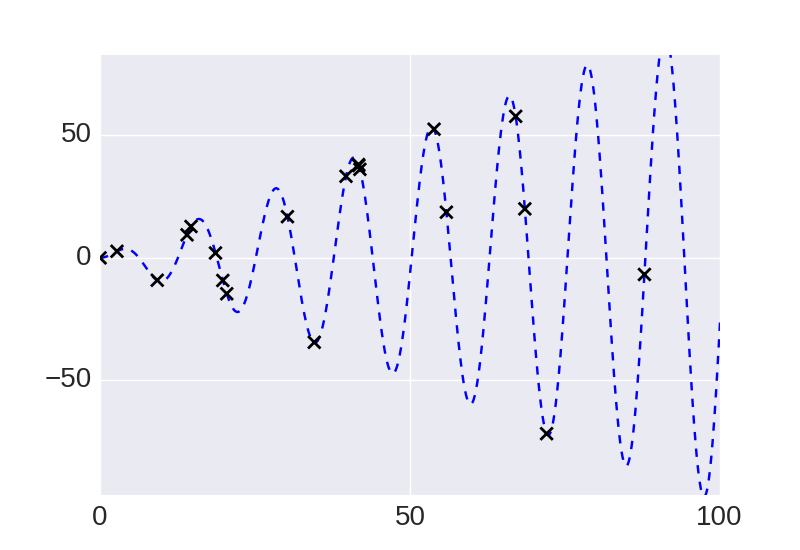
\includegraphics[width=\textwidth]{figs/composition/composition_demo_raw_data.png}
        \caption{Raw Data}
    \end{subfigure}
    ~ %add desired spacing between images, e. g. ~, \quad, \qquad, \hfill etc. 
      %(or a blank line to force the subfigure onto a new line)
    \begin{subfigure}[b]{0.45\textwidth}
\small
     \begin{align*}
    \text{LIN} &=   \sigma_1^2(x x^\prime)\\
    \text{PER} &=  \sigma_2^2 \exp \bigg( \frac{2 \sin^2 ( \pi (x - x^\prime)/p}{\ell^2} \bigg)\\ 
    \text{LIN} \times \text{PER} &=  \sigma_1^2(x x^\prime)\, \sigma_2^2 \exp \bigg( \frac{2 \sin^2 ( \pi (x - x^\prime)/p}{\ell^2} \bigg) 
    \end{align*}\vspace{5mm} 
        \caption{Kernels}
    \end{subfigure}\vspace{4mm} 


Parameterized Kernels:\vspace{3mm} 

     \begin{subfigure}[b]{0.3\textwidth}
      \centering \footnotesize
       $20.1^2(x x^\prime) $ \vspace{2mm}
	\caption{LIN}
    \end{subfigure}
    ~ %add desired spacing between images, e. g. ~, \quad, \qquad, \hfill etc. 
      %(or a blank line to force the subfigure onto a new line)
    \begin{subfigure}[b]{0.3\textwidth}
      \centering \footnotesize
      $19.1^2 \exp \bigg( \frac{2 \sin^2 ( \pi (x - x^\prime)/37.7}{6.3^2} \bigg)$ 
	\caption{PER}
    \end{subfigure}
    ~ %add desired spacing between images, e. g. ~, \quad, \qquad, \hfill etc. 
    %(or a blank line to force the subfigure onto a new line)
    \begin{subfigure}[b]{0.3\textwidth}
    \centering \footnotesize
      $383.9^2 (x x^\prime) \exp \bigg( \frac{2 \sin^2 ( \pi (x - x^\prime)/37.7}{6.3^2} \bigg)$ 
        \caption{LIN $\times$ PER}
    \end{subfigure} \vspace{4mm} 

Prior:

     \begin{subfigure}[b]{0.3\textwidth}
        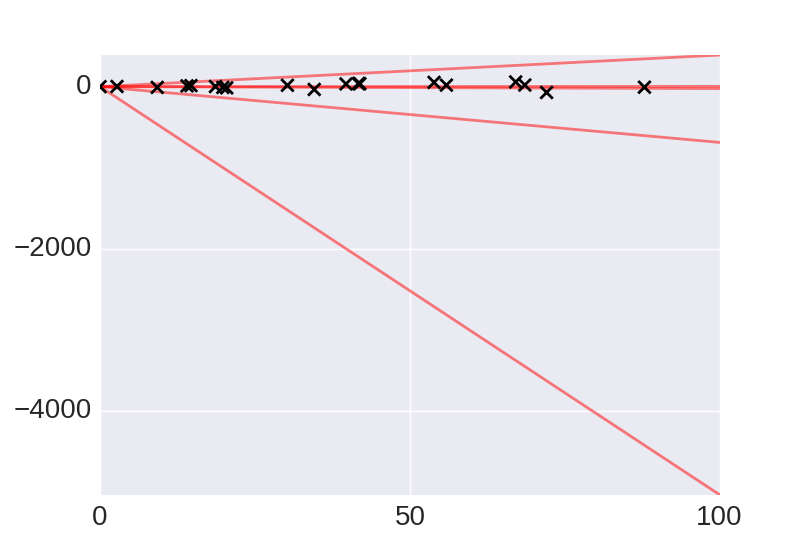
\includegraphics[width=\textwidth]{figs/composition/composition_demo_LIN_prior.png}
        \caption{LIN}
    \end{subfigure}
    ~ %add desired spacing between images, e. g. ~, \quad, \qquad, \hfill etc. 
      %(or a blank line to force the subfigure onto a new line)
    \begin{subfigure}[b]{0.3\textwidth}
        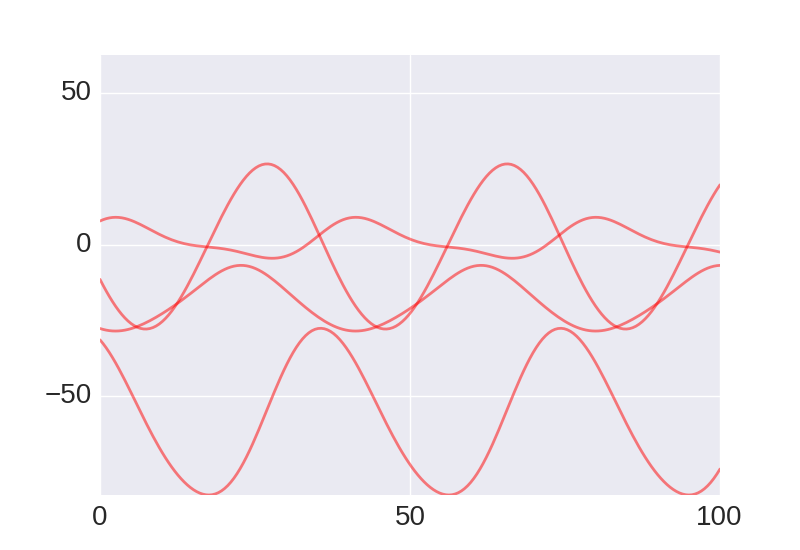
\includegraphics[width=\textwidth]{figs/composition/composition_demo_PER_prior.png}
        \caption{PER}
    \end{subfigure}
    ~ %add desired spacing between images, e. g. ~, \quad, \qquad, \hfill etc. 
    %(or a blank line to force the subfigure onto a new line)
    \begin{subfigure}[b]{0.3\textwidth}
        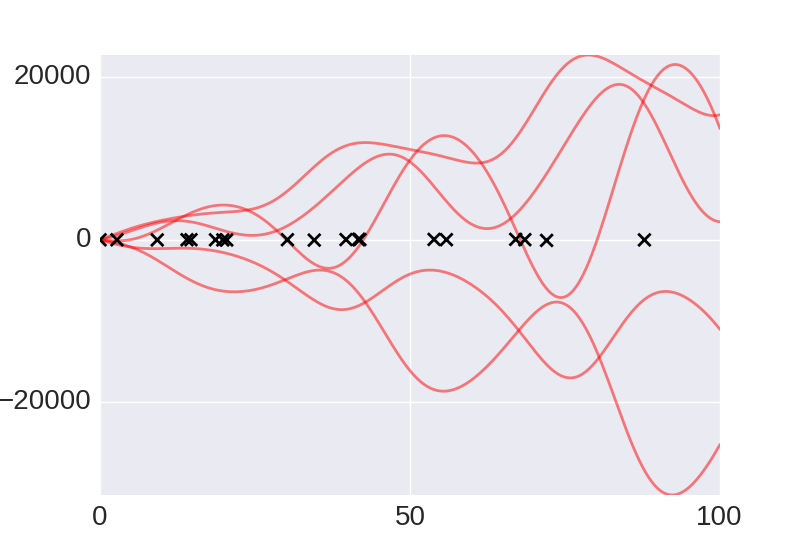
\includegraphics[width=\textwidth]{figs/composition/composition_demo_LINxPER_prior.png}
        \caption{LIN $\times$ PER}
    \end{subfigure} \vspace{4mm} 

Posterior:

 \begin{subfigure}[b]{0.3\textwidth}
        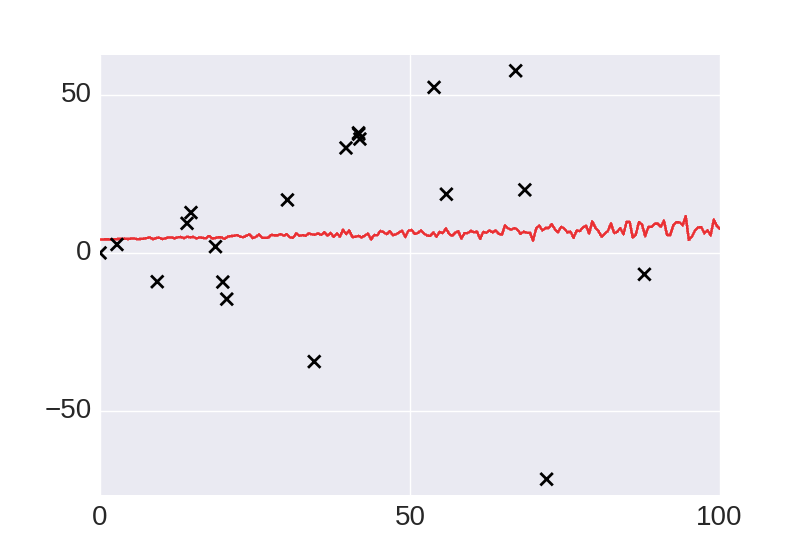
\includegraphics[width=\textwidth]{figs/composition/composition_demo_LIN.png}
        \caption{LIN}
    \end{subfigure}
    ~ %add desired spacing between images, e. g. ~, \quad, \qquad, \hfill etc. 
      %(or a blank line to force the subfigure onto a new line)
    \begin{subfigure}[b]{0.3\textwidth}
        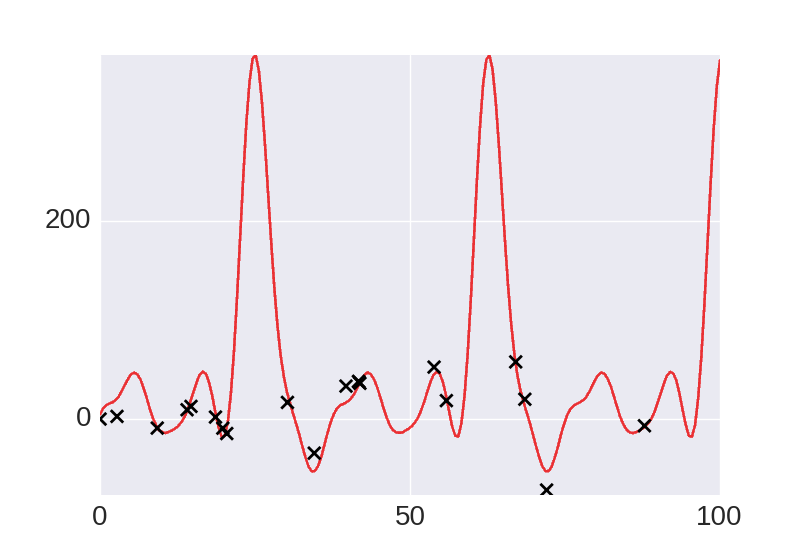
\includegraphics[width=\textwidth]{figs/composition/composition_demo_PER.png}
        \caption{PER}
    \end{subfigure}
    ~ %add desired spacing between images, e. g. ~, \quad, \qquad, \hfill etc. 
    %(or a blank line to force the subfigure onto a new line)
    \begin{subfigure}[b]{0.3\textwidth}
        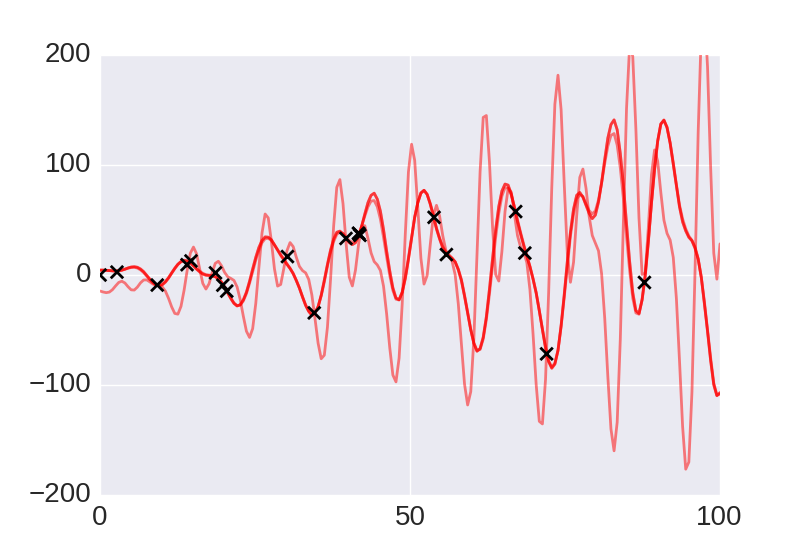
\includegraphics[width=\textwidth]{figs/composition/composition_demo_LINxPER.png}
        \caption{LIN $\times$ PER}
    \end{subfigure}

%20.0739791735
%6.31647597198
%37.7184218042
%19.1051376016

\caption{We depict kernel composition. 
(a) shows raw data (black) generated with a sine function with linearly growing amplitude (blue).
This data is used for all the plots (c-h). 
(b) shows the linear and the periodic base kernel as well as a composition of both. 
The multiplication of the two kernels indicates local interaction. The local interaction we account for in this case is the growing amplitude (a). For each column (c-h) $\bm{\theta}$ is different.(c-e) show samples from the prior
prior predictive $\fbf_*$ where random parameters are used, that is, we sample before any data points are observed.
(f-h) show samples from the predictive posterior $\hat\fbf$, after the data has been observed.}
\label{fig:composition_tutorial}
\end{figure}
%%%%%%%%%%%%%%%%%%%%%%%%%%%%%%%%%%%%%%%%%%%%%%%%%%%%%%%%%%%%
These high-level properties are compositional via addition and multiplication of different covariance functions. 
That means that we can also combine these properties.
By using multiplication of kernels we can model a local interaction of two components, for example 
%%%%%%%%%%%%%%%%%%%%%%%%%%%%%%%%%%%%%%%%%%%%%%%%%%%%%%%%%%%%
\begin{equation}\label{eq:LINxPER}
    \text{LIN} \times \text{PER} =  \sigma_1^2(x x^\prime)\, \sigma_2^2 \exp \bigg( \frac{2 \sin^2 ( \pi (x - x^\prime)/p}{\ell^2} \bigg) 
\end{equation}
%%%%%%%%%%%%%%%%%%%%%%%%%%%%%%%%%%%%%%%%%%%%%%%%%%%%%%%%%%%%
This results in a combination of the higher level properties of linearity and  periodicity.
In Fig \ref{fig:composition_tutorial} (e) we depict samples for $\fbf_*$ that are periodic
with linearly increasing amplitude.
We consider this a local interaction because the actual interaction depends on the similarity
of two data points.
An addition of covariance functions models a global interaction, that is an interaction of two high-level components that is qualitatively not dependent on the input space. An example for this a periodic function with a linear
trend.

Covariance functions come with  free parameters that we call hyper-parameters which we will
refer to as $\bm{\theta}$.
For each kernel type, each $\bm{\theta}$ is different, that is, in (\ref{eq:LIN1}) we have $\thetabf=\{\sigma_1\}$,
in (\ref{eq:PER1}) we have $\bm{\theta}=\{\sigma_2,p,\ell\}$ and in 
(\ref{eq:LINxPER}) we have $\bm{\theta}=\{\sigma_1,\sigma_2,p,\ell\}$.
Adjusting these hyper-parameters changes lower level qualitative attributes such as length
scales ($\ell$) while preserving the higher level qualitative properties of the distribution
such as linearity.
We write the parameterized covariance function as $\mathbf{K}_{\bm{\theta}}(\xbf,\xbf)$ and the
covariance matrix determined by a parameterized covariance function as $\mathbf{K}_{\bm{\theta}}$.

When we observe the data, that is we condition on the input-output pairs $\{\xbf,\fbf\}$ we can sample from the 
predictive posterior $P(\hat\fbf \mid \fbf)$ given $\mathbf{K}_{\bm{\theta}}$ and respectively $\bm{\hat{\mu}}$ and $\hat{\mathbf{K}}_{\bm{\theta}}$.
If we choose suitable parameters, for example by performing inference, we can capture the underlying dynamics of the data well (see Fig. \ref{fig:composition_tutorial} (f-h)) while sampling $\hat{\fbf}$.
Note that goodness of fit is not only limited to the parameters. A too simple qualitative structure
implies unsuitable behaviour, as for example in (Fig. \ref{fig:composition_tutorial} (g)) where additional 
recurring spikes are introduced to account for the changing amplitude of the true function that 
generated the data.







%\subsection{A Bayesian interpretation}
%We illustrate and compare Bayesian and frequentist view points on GP with a simple example (Fig. \ref{fig:BayesVSFreq}). We show how in a simple model, two outliers can bias a maximum a posteriori inference. The data where generated with:
\begin{equation}
\label{eq:line1}
y = 2x + 15
\end{equation}
and outliers are generated with a parallel line:
\begin{equation}
\label{eq:line2}
\hat{y} = 2x + 40.
\end{equation}
We add some small amount of white noise. We generate eight data points with (\ref{eq:line1}) and two with (\ref{eq:line2}). Since we suspect the underlying data generating mechanism to be linear, we fit a linear kernel with a constant covariance as intercept and some white noise:
\begin{equation}
\mathbf{K} = \text{LIN} + \text{C} + \text{WN}.
\end{equation}
where we upper case matrix notation denotes the covariance matrix of the complete training data. Omitting the scaling parameter for the linear kernel, there are two hyperparameters to learn, that is the noise variance and the hyper-parameter for the constant function. Maximum a posteriori inference fits the single one best line and accounts for the outliers with a large noise scaling parameter. MH does better. It assigns a small amount of probability mass to a different scaling parameter and a larger constant. The resulting prediction (indicating with the predictive mean in figure \ref{fig:BayesVSFreq}) is closer to the true underlying function.   

\begin{figure}
        \centering
        \begin{subfigure}[b]{0.49\textwidth} \centering
              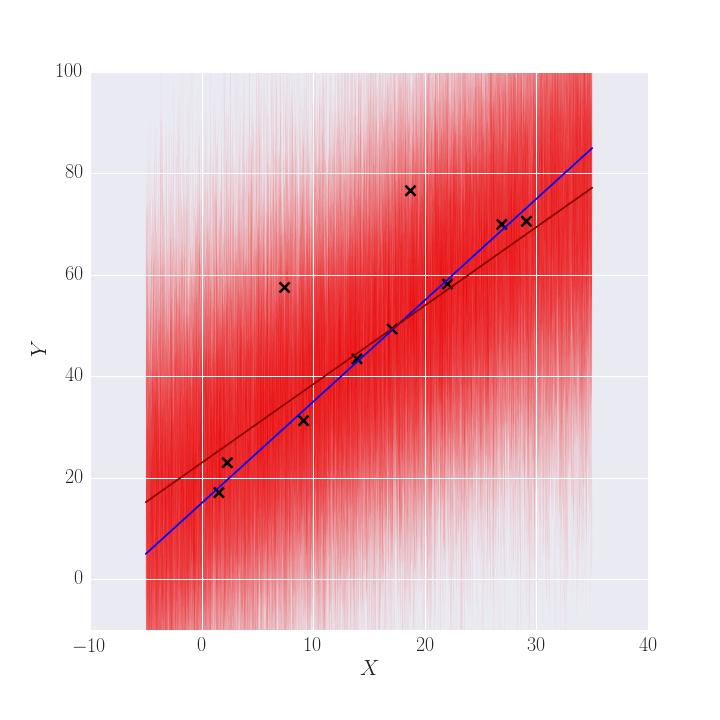
\includegraphics[height=7.5cm]{figs/MAP_linear.png}
              \caption{MAP}
                \label{fig:maplin}
        \end{subfigure}%
        \begin{subfigure}[b]{0.49\textwidth} \centering
            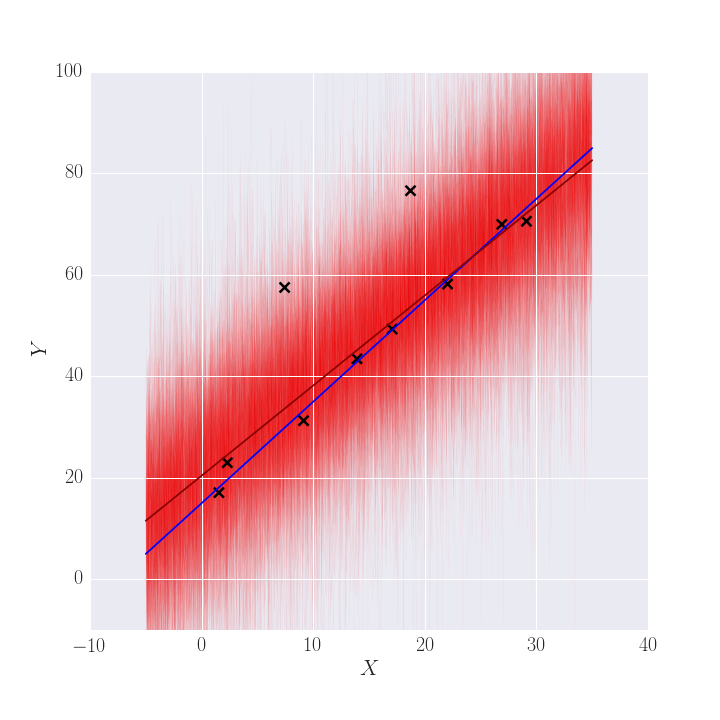
\includegraphics[height=7.5cm]{figs/MH_linear.png}
            \caption{MH}
                \label{fig:mhlin}
        \end{subfigure}%
        \caption{(a) depicts MAP inference on the data, (b) depicts MH for hyperparameter inference. The blue line is the actual data generating function. Red are samples drawn from the posterior. The dark red line is the posterior predictive mean. We see that the MH shifts the posterior closer to the ground truth than MAP.  }\label{fig:BayesVSFreq}
\end{figure}


\subsection{Packaging Gaussian Processes for Venture}
Random samples from a \ac{GP}, like all random samples in Venture programs,
are generated with the invocation of \ac{SP}s.
Such \ac{SP}s accept input arguments that are values in Venture and sample output
values given those inputs. A \ac{PSP} is the most basic unit of computation in
Venture. It can be deterministic or random. If a \ac{PSP} is random then it can simulate from a family of
distributions. In addition to simulating,
a random PSPs may be able to report the log-density of an output given an input.
Different \ac{PSP}s and \ac{SP}s are used to construct the \ac{GP} interface:
\begin{enumerate}
\item MakeGPOutputPSP is a deterministic PSP whose output is a \ac{GP}, namely the
GPSP, given a
covariance and a mean function as input. Inputting a mean function is optional,
if it is not supplied, it is set to constant 0.

\item GPSP of is type SP. GPSP can \ac{AAA}. \ac{AAA}-\ac{SP}s can keep track of
their outputs and report
the joint log-density of all of its applications. This is crucial so that we do
not need to visit all of the dependent units of computation to explicitly account for their
log-densities. For Venture, the construction of the scaffold, that is the
factoring of global inference problems into coherent sub-problems, can stop upon
reaching an \ac{AAA} node. GPSP is responsible for tracking the sufficient statistics
from the applications of GPSP and for evaluating the log density of all those
applications as a block. It also constructs the auxiliary SP (SPAux).
\item GPSPAux of type SPAux. An auxiliary SP is stateless but comes with an auxiliary
store that carries mutable information. In case of the \ac{GP} it tracks the
samples that were incorporated.
\item GPOutputPSP of type Random PSP.  It is this SP that actually samples
regression output at given input.
\end{enumerate}


%procedures that return other stochastic procedures and implement this optimization are said to be
%absorbing at applications, often abbreviated AAA.




\section{Gaussian Process Memoization in Venture}
Memoization is the practice of storing previously computed values of a function so that future calls with the same inputs can be evaluated by lookup rather than re-computation.
To transfer this idea to probabilistic programming, we now introduce a language construct called a
\emph{statistical memoizer}.  Suppose we have a function $\ftt$ which can be evaluated 
but we wish to learn about the behavior of $\ftt$ using as
few evaluations as possible.  The statistical memoizer, which here we give the
name \gpmem, was motivated by this purpose.  It produces two outputs:
\[ \ftt \xrightarrow{\gpmem} (\ftt_{\text{compute}}, \ftt_\emu). \]
The function $\ftt_{compute}$ calls $\ftt$ and stores the output in a memo
table, just as traditional memoization does.  The function $\ftt_\emu$ is
an online statistical emulator which uses the memo table as its training
data.  A fully Bayesian emulator, modelling the true function $\ftt$ as a
random function $f \sim P(f)$, would satisfy
\[
\texttt{(}\ftt_\emu\ \xtt_1\ \ldots\ \xtt_k\texttt{)}
\sim
P\pn{
  f(\xtt_1), \ldots, f(\xtt_k)
  \mvert
  \text{$f(\xtt) = \texttt{(f x)}$ for each $\xtt$ in memo table}
}.
\]
Different implementations of the statistical memoizer can have
different prior distributions $P(f)$; in this paper, we deploy a \ac{GP} 
prior (implemented as \texttt{gpmem} below).  Note that we require the ability
to sample $\ftt_\emu$ jointly at multiple inputs because the values of
$f(\xtt_1),\ldots,f(\xtt_k)$ will in general be dependent.


\begin{figure}
\centering
% for double arrows a la chef
% adapt line thickness and line width, if needed
\begin{tikzpicture}[thick]
\node[] (start) {};
 \node[draw,circle,minimum size=1.5cm,left = 0.5cm of start] (f) {f$_{\text{compute}}$};
 \node[draw,right = 0.5cm of start,circle,minimum size=1.5cm] (K) {$\mathbf{K}_{\theta}$};
 %\node[below left of=f_K,xshift=-1.7cm,yshift=-0.1cm] (theta) {$\bm{\theta} \sim P(\bm{\theta})$};
 \node[draw,rectangle,below=1.5cm of start, text width = 6.6cm] (gpmem) {\centering\texttt{gpmem}\vspace{2mm}
 
\small$\text{memo table} = (\mathbf{x}_{past},\mathbf{y}_{past})$\vspace{1.5mm}
 
 
\small$P(f_{emu}(x) \mid \mathbf{x}_{past},\mathbf{y}_{past})\sim \mathcal{N}(\mu(\mathbf{x}),\mathbf{K}_\theta\big(\mathbf{x},\mathbf{x})\big)$
 };
%  \node[draw,rectangle,color=ForestGreen,below = .1ex of gpmem,minimum width=1.5cm, minimum height=0.4cm,yshift=0.9cm,xshift=0.3cm] (mark) {};
  \node[draw,rectangle,dashed,right=2.2cm of K, text width = 2.2cm] (math) {\small
 $\mathbf{K}_{\theta} = \text{SE}(x,x^\prime)$\vspace{1.5mm}
 
 $\theta \;\;\,\,= \{sf,\ell \}$\vspace{1.5mm}
 
 $sf\;\, \sim P(sf)$\vspace{1.5mm}

 $\ell\;\;\;\; \sim P(\ell)$\vspace{1.5mm}
 
 
%\scriptnotesize
%
%%$\mu(\mathbf{x}) =\mu(\mathbf{x}) + \mathbf{K}_\theta(\mathbf{x},\mathbf{x}_{past})\mathbf{K}_\theta(\mathbf{x}_{past},\mathbf{x}_{past})^{-1}(\mathbf{y}_{past} - \mu(\mathbf{x}_{past}))$
 };
 \node[draw,rectangle,dashed,minimum size=1cm,left= 2.2cm of f] (resources) {
\includegraphics[width=3cm]{figs/resources.png}};

\node[draw,rectangle,below=1cm of gpmem,text width =7cm] (f_emu) {\centering $f_{emu}$ \vspace{2mm}

\begin{tabular}{l|l}\small
  $x$ & $f(x)$ \\ \hline
   $x_1$  & $y_1$ \\ 
   $x_2$  & $y_2$ \\
  $\cdots$ &   $\cdots$
 \end{tabular}
 $\;\;\;\;$
 \begin{tabular}{l}
 Parameters:\\
\small  Kernel lengthscale $\ell$  \\
\small Kernel scale-factor $sf$
 \end{tabular}

};
%\node[right = 1.2 cm of f_emu,inner sep = 0pt,outer sep=0pt,minimum size=25pt] (emu_annotate) {Infer: $\theta\;$};

\node[below = .1ex of gpmem,inner sep = 0pt,outer sep=0pt,xshift=-0.3cm] (helper1) {};
\node[below = .1ex of gpmem,inner sep = 0pt,outer sep=0pt,xshift=0.7cm] (helper2) {};

\node[above = .1ex of f_emu,inner sep = 0pt,outer sep=0pt, xshift=0mm] (helper_emu) {};

\node[above = 0.75cm of resources,inner sep = 0pt,outer sep=0pt] (helper_resource_top) {};
\node[left = 1cm of f_emu] (x_hat) {$\hat{x}$} ;
\node[right = 1cm of f_emu] (GaussianHat) {$\mathcal{N}(\hat{\bm\mu},\hat{\mathbf{K}})$} ;

%\node[right =1. cm  of f_emu, yshift=1.5cm] (infer) {\small Infer: $\ell$, $sf$} ;

% 1st pass: draw arrows

  \draw[thick,dashed,->] (resources) --node [pos=0.5,below] {resource}  node [pos=0.5,above] {outside} (f);
  \draw[thick,dashed,->] (math) -- node [pos=0.5,above] {Kernel} (K);
  \draw[thick,->] (K) -- (gpmem);
  \draw[thick,->] (f) -- (gpmem);
 % \draw[thick,->] (theta) -- (gpmem);
  \draw[thick,->] (gpmem) -- (f_emu);

 % \draw[thick,->,color=ForestGreen] (helper_compute) -- node[pos=0.5, sloped, below] {probe} (helper1);
 % \draw[thick,->,color=ForestGreen] (helper2) -- node[pos=0.5, sloped,above] {improves} (helper_emu);
   % \draw[thick,->,dashed,color=ForestGreen] (helper_resource) -- node[pos=0.5,above] {$f_{com}(x_2)=y_2$} (f_compute);
  %  \draw[thick,->,dashed,color=ForestGreen] (helper_resource) -- (resources);
     \draw[thick,->,dashed] (x_hat) -- (f_emu); 
     \draw[thick,->,dashed] (f_emu) -- (GaussianHat); 
 % \draw[thick,->] (theta) -- (gpmem);
  
   
%\path[](f_emu) edge [in=90, out=50,thick] (emu_annotate)
%    (emu_annotate) edge [->,in=310, out=270,thick]  (f_emu);
  % Note: If you have no branches, the 2nd pass is not needed

\end{tikzpicture}


\begin{tabular}{ll}
% line 1
& \\
\hline
\begin{lstlisting}[mathescape,escapechar=\#]
define f = proc( x) {
		    exp(-0.1*abs(x-2))) *
		    10* cos(0.4*x) + 0.2
		    }    
assume (f_compute f_emu) =  gpmem( f, K)
sample f_emu( array( -20, $\cdots$, 20)) 

\end{lstlisting}
& \raisebox{-0.5\height}{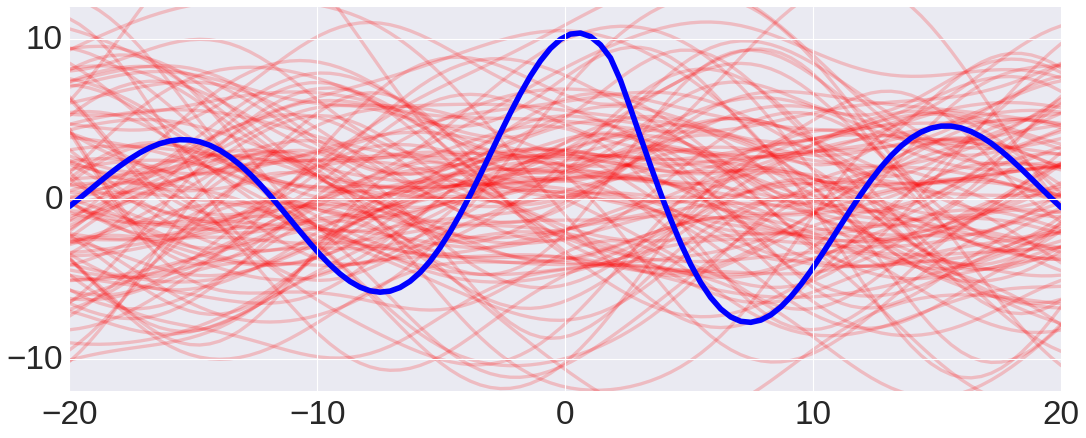
\includegraphics[height=2.5cm]{figs/tutorial_1.png}} \\ \hline
% line 2
\begin{lstlisting}[mathescape,escapechar=\#]
predict f_compute( 12.6)

sample f_emu( array( -20, $\cdots$, 20)) 

\end{lstlisting}
 &  \raisebox{-0.5\height}{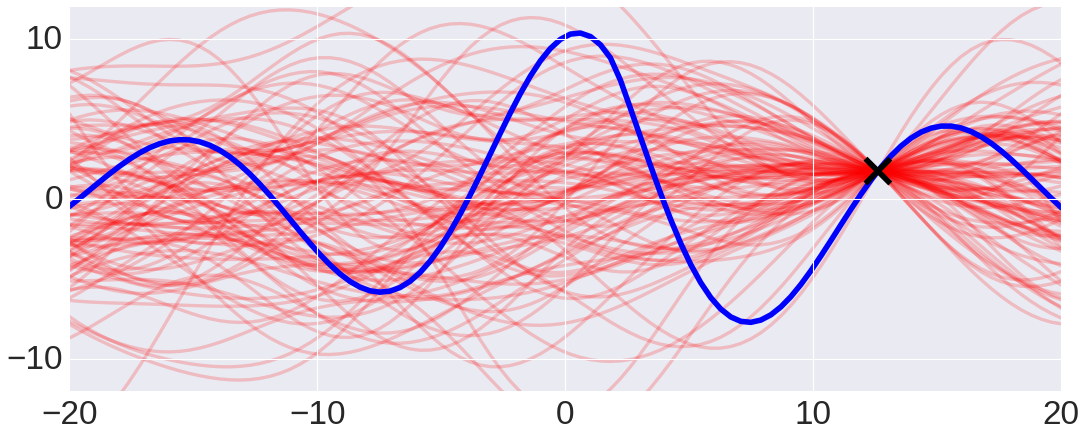
\includegraphics[height=2.5cm]{figs/tutorial_2.png}}  \\ \hline
% line 3 
 \begin{lstlisting}[mathescape,escapechar=\#]
predict f_compute( -6.4)

sample f_emu( array( -20, $\cdots$, 20)) 

\end{lstlisting}
 &  \raisebox{-0.5\height}{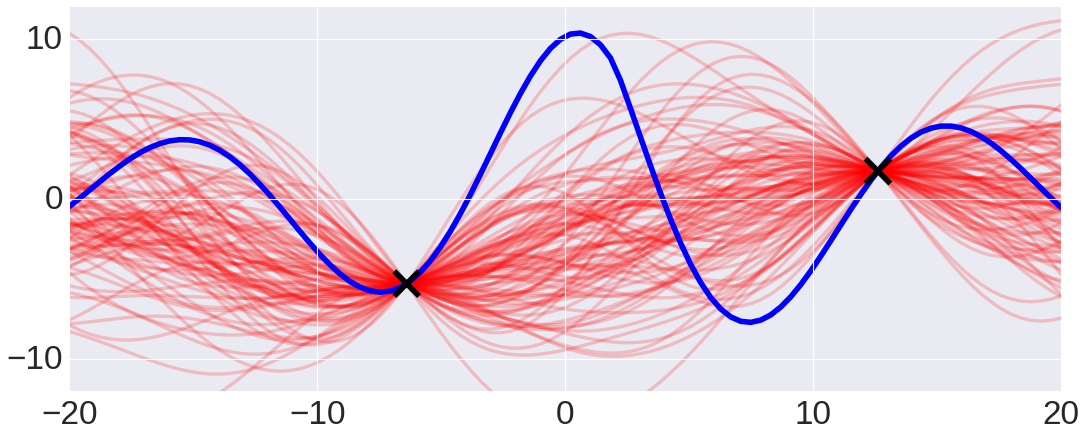
\includegraphics[height=2.5cm]{figs/tutorial_3.png}}  \\ \hline
% line 4
 \begin{lstlisting}[mathescape,escapechar=\#]
observe f_emu( -3.1) = 2.60 
observe f_emu( 7.8) = -7.60  
observe f_emu( 0.0) =  10.19

sample f_emu( array( -20, $\cdots$, 20)) 
  
\end{lstlisting}
 &   \raisebox{-0.5\height}{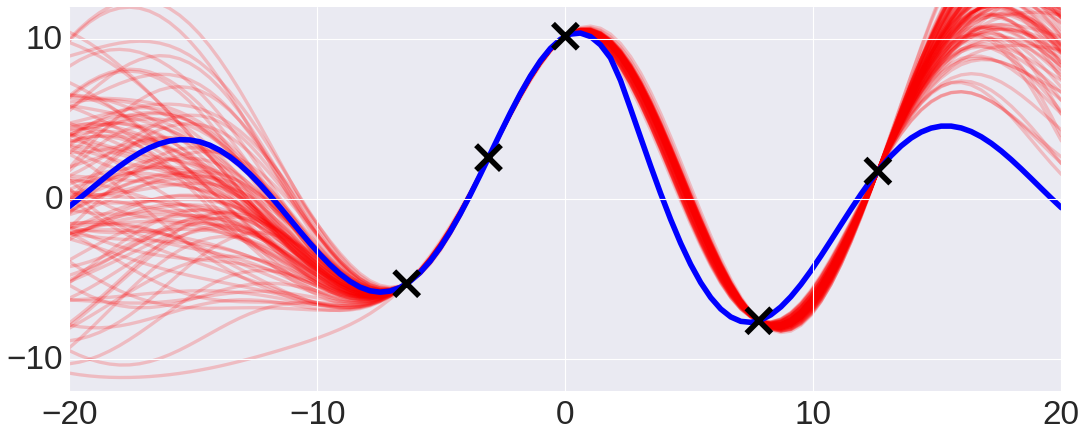
\includegraphics[height=2.5cm]{figs/tutorial_5.png}} \\ \hline
% line 5
 \begin{lstlisting}[mathescape,escapechar=\#]
infer mh(quote(hyper-parameter), one, 50)

sample f_emu( array( -20, $\cdots$, 20)) 
  
\end{lstlisting}
 &   \raisebox{-0.5\height}{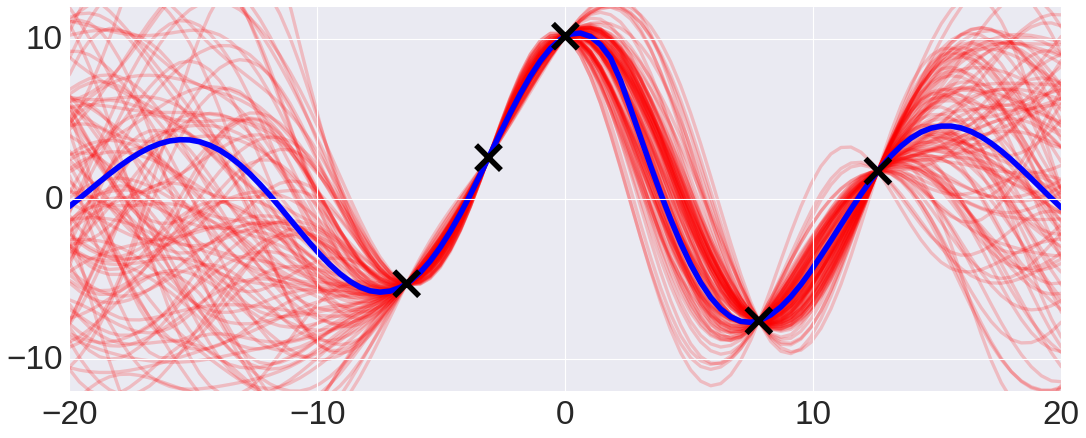
\includegraphics[height=2.5cm]{figs/tutorial_6.png}}
\end{tabular}
%\put(-245,10){\line(1,0){200}}
\put(-33,77){\color{ForestGreen}\thicklines \vector(0,-1){15}}
\put(-96,6){\color{ForestGreen}\thicklines \vector(0,-1){15}}
\put(-48,-63){\thicklines \vector(0,-1){15}}
\put(-84,-43){\thicklines \vector(0,-1){15}}
\put(-73,-68){\thicklines \vector(0,1){15}}
\put(-460,110){(b)}
\put(-460,45){(c)}
\put(-460,-10){(d)}
\put(-460,-75){(e)}
\put(-460,-130){(f)}
\caption{\small \gpmem\ tutorial. The top shows a schematic of \gpmem.
  \texttt{f\_compute} probes an outside resource.
  This can be expensive (top left).
  Every probe is memoized and improves the emulator. Below the schematic we see the evolution
  of \gpmem's state of believe of the world given certain Venture
  directives. On the right, we depict the true function (blue), samples from the emulator (red) and incorporated observations (black).}
\label{fig:gpmem_tutorial}
\end{figure}

% Panel 1
We explain how \gpmem, the statistical memoizer with \ac{GP}-prior, works using a simple tutorial
(Fig. \ref{fig:gpmem_tutorial}). 
The top panel of this figure sketches the schematic of \gpmem.
$\ftt$ is the aforementioned function which can be evaluated using resources that potentially come
from outside of Venture.  
We feed this function into \gpmem\ alongside
a parameterised kernel $\mathbf{K}$. The hyper-parameters for this kernel are sampled from a 
prior distribution which is depicted in the top right box. 
We use a squared exponential covariance function:
\[
\text{SE} = \sigma^2 \exp(-\frac{(x-x^\prime)^2}{2\ell^2})
\]
Note that we annotate $\bm{\theta}=\{\texttt{sf},\texttt{l}\}$ for subsequent
inference as belonging to (i) the scope "hyper-parameter" and (ii) blocks 0 and 1 respectively.

\gpmem\ implements a memoization table, where all previously
computed function evaluations are stored. We also initialize a \ac{GP}-prior that
will serve as our statistical emulator.
All value pairs stored in the memoization table are incorporated as observations of
the \ac{GP}.
The emulator allows us to make probabilistic predictions on function evaluations.
We simply feed the regression input
into the emulator and output a predictive posterior Gaussian distribution determined by the \ac{GP} and
the memoization table.

% Panel 2
We can either define the function f that serves as as input for \gpmem\
 natively in Venture
(as shown in the second panel Fig. \ref{fig:gpmem_tutorial}) or we interleave Venture with foreign code. 
This can be useful when $\ftt$ is computed with the help of outside resources.
Before making any observations or calls to $\ftt$
we can sample from the prior at the inputs from -20 to 20 using the emulator:
    \begin{lstlisting}
    assume (f_compute, f_emu) = gpmem(f, K))

    sample f_emu(array(-20, ..., 20))
    \end{lstlisting}
% Panel 3
In the following panel of Fig. \ref{fig:gpmem_tutorial}, we probe the external function $\ftt$ at point 12.6 and memoize it's result by calling 
   \begin{lstlisting}
    predict f_compute (12.6).
    \end{lstlisting}
When we subsequently sample from the emulator, we now compute the \ac{GP} posterior which shifts from uncertainty to near certainty close to the input 12.6.

% Panel 4
We can repeat the process at a different point (probing point -6.4 in the fourth panel of Fig. \ref{fig:gpmem_tutorial}) to see that we gain certainty about another part of the curve. 

% Panel 5
We can add information to $\texttt{f}_\text{emu}$ about presumable value pairs of $\ftt$ without calling $\texttt{f}_\text{compute}$
(fifth panel, Fig. \ref{fig:gpmem_tutorial}).
If a friend tells us the value of $\ftt$ we can call observe to store this information in the incorporated observations for $\texttt{f}_\text{emu}$ only:
    \begin{lstlisting}
    observe f_emu( -3.1) = 2.60.
    \end{lstlisting}
We have this value pair now available for the computation of the \ac{GP} posterior. 
For sampling with the emulator, the effect is the same as calling predict with the $\texttt{f}_\text{compute}$.
However, we can imagine at least one scenario where such as distinction in the treatment of observations 
is beneficial. Let us say we do not only have the real function available but also a domain expert with knowledge 
about this function.
This expert could tell us what the value is at a given input.
Potentially, the value provided by the expert could disagree with the value computed with $\ftt$ for example 
due to different levels of observation noise. 

% Panel 6
Finally, we can update our posterior by inferring the posterior over hyper-parameter values.
We can take 50 \ac{MH} steps by calling that where we take an \ac{MH} steps for either of the two blocks for the scope "hyper-parameter": 
   \begin{lstlisting}
    infer mh( 'hyper-parameter, one, 50).
    \end{lstlisting}
The newly inferred hyper-parameters allow us now adequately reflect uncertainty about the curve given all incorporated observations (compare bottom panel on the right with the samples before inference, one panel above).


\section{Applications}
This paper illustrates the flexibility of \gpmem\ by showing how it can concisely encode three different applications of \ac{GP}s.
The first is a standard example from hierarchical Bayesian statistics, where Bayesian inference over a hierarchical hyper-prior is used to provide a curve-fitting methodology that is robust to outliers.
The second is a structure learning application from probabilistic artificial intelligence, where \ac{GP}s are used to discover qualitative structure in time series data.
The third is a reinforcement learning application, where \ac{GP}s are used as part of a Thompson sampling formulation of Bayesian optimization for general real-valued objective functions with real inputs.

\subsection{Nonlinear regression in the presence of outliers}

The probability of the hyper-parameters of a GP with assumptions as above and given covariance function structure $\mathbf{K}$ can be described as:
\begin{equation}
\label{eq:hyperProbability}
P(\bm{\theta} \mid \mathbf{D,K}) = \frac{P(\mathbf{D} \mid \bm{\theta}, \mathbf{K})P(\bm{\theta} \mid  \mathbf{K})}{P(\mathbf{D} \mid \mathbf{K})}.
\end{equation}
Let the $\mathbf{K}$ be the sum of a smoothing and a white noise (WN) kernel. For this case, Neal suggested the problem of outliers in data as a use-case for a hierarchical Bayesian treatment of Gaussian processes~\citeyearpar{neal1997monte}\footnote{In \citep{neal1997monte} the sum of an SE plus a constant kernel is used. We stick to the WN kernel for illustrative purposes.}. The work suggests a hierarchical system of hyper-parameterization. Here, we draw hyper-parameters from a $\Gamma$ distributions:
\begin{equation}
\ell^{(t)} \sim \Gamma(\alpha_1,\beta_1),\;\sigma^{(t)} \sim \Gamma(\alpha_2,\beta_2)
\end{equation} 
and in turn sample the $\alpha$ and $\beta$ from $\Gamma$ distributions as well:
\begin{equation}
\alpha_1^{(t)} \sim \Gamma(\alpha^1_{\alpha},\beta^1_{ \alpha } ),\; \alpha_2^{(t)} \sim \Gamma(\alpha^2_{\alpha},\beta^2_{\alpha}),\cdots
\end{equation}
Assuming the covariance structure is an additive comprised of a smoothing and a white noise kernel, one can represent this kind of model using \gpmem\ with only a few lines of code:
\begin{minipage}{\linewidth}
\belowcaptionskip=-10pt
\begin{lstlisting}[frame=single,mathescape,label=alg:gphierarch,basicstyle=\selectfont\ttfamily]
/// SETTING UP THE MODEL
assume alpha_sf = tag('hyperhyper, gamma(7, 1))
assume beta_sf = tag('hyperhyper, gamma(7, 1))
assume alpha_l = tag('hyperhyper, gamma(7, 1))
assume beta_l = tag('hyperhyper, gamma(7, 1))

// Parameters of the covariance function
assume sf = tag('hyper, gamma(alpha_sf, beta_sf)))
assume l = tag('hyper, gamma(alpha_l, beta_l)))
assume sigma = tag('hyper, uniform_continuous(0, 2)) 

// The covariance function
assume se = make_squaredexp(sf, l)
assume wn = make_whitenoise(sigma)
assume composite_covariance = add_funcs(se, wn)

/// PERFORMING INFERENCE
// Create a prober and emulator using gpmem
assume f_restr = get_neal_blackbox()
assume (f_compute, f_emu) = gpmem(f_restr, composite_covariance)

// Probe all data points
predict mapv(f_compute, get_neal_data_xs())

// Infer hypers and hyperhypers
infer repeat(100, do(
    mh('hyperhyper, one, 2),
    mh('hyper, one, 1)))

\end{lstlisting}
\end{minipage}

Neal provides a custom inference algorithm setting and evaluates it using the following synthetic data problem. Let $f$ be the underlying function that generates the data:
\begin{equation}
f(x) =  0.3 + 0.4 x + 0.5 \sin(2.7x) + \frac{1.1}{(1+ x^2)} + \eta \;\;\; with\;\;\eta \sim \mathcal{N}(0,\sigma)
\end{equation}
We synthetically generate outliers by setting $\sigma = 0.1$ in $95\%$ of the cases and to $\sigma = 1$ in the remaining cases. \gpmem\  can capture the true underlying function within only 100 MH steps on the hyper-parameters to get a good approximation for their posterior (see Fig. \ref{fig:neal}). Note that Neal devices an additional noise model and performs large number of Hybrid-Monte Carlo and Gibbs steps.  
\begin{figure}
        \centering

        \begin{subfigure}[b]{0.49\textwidth} \centering
                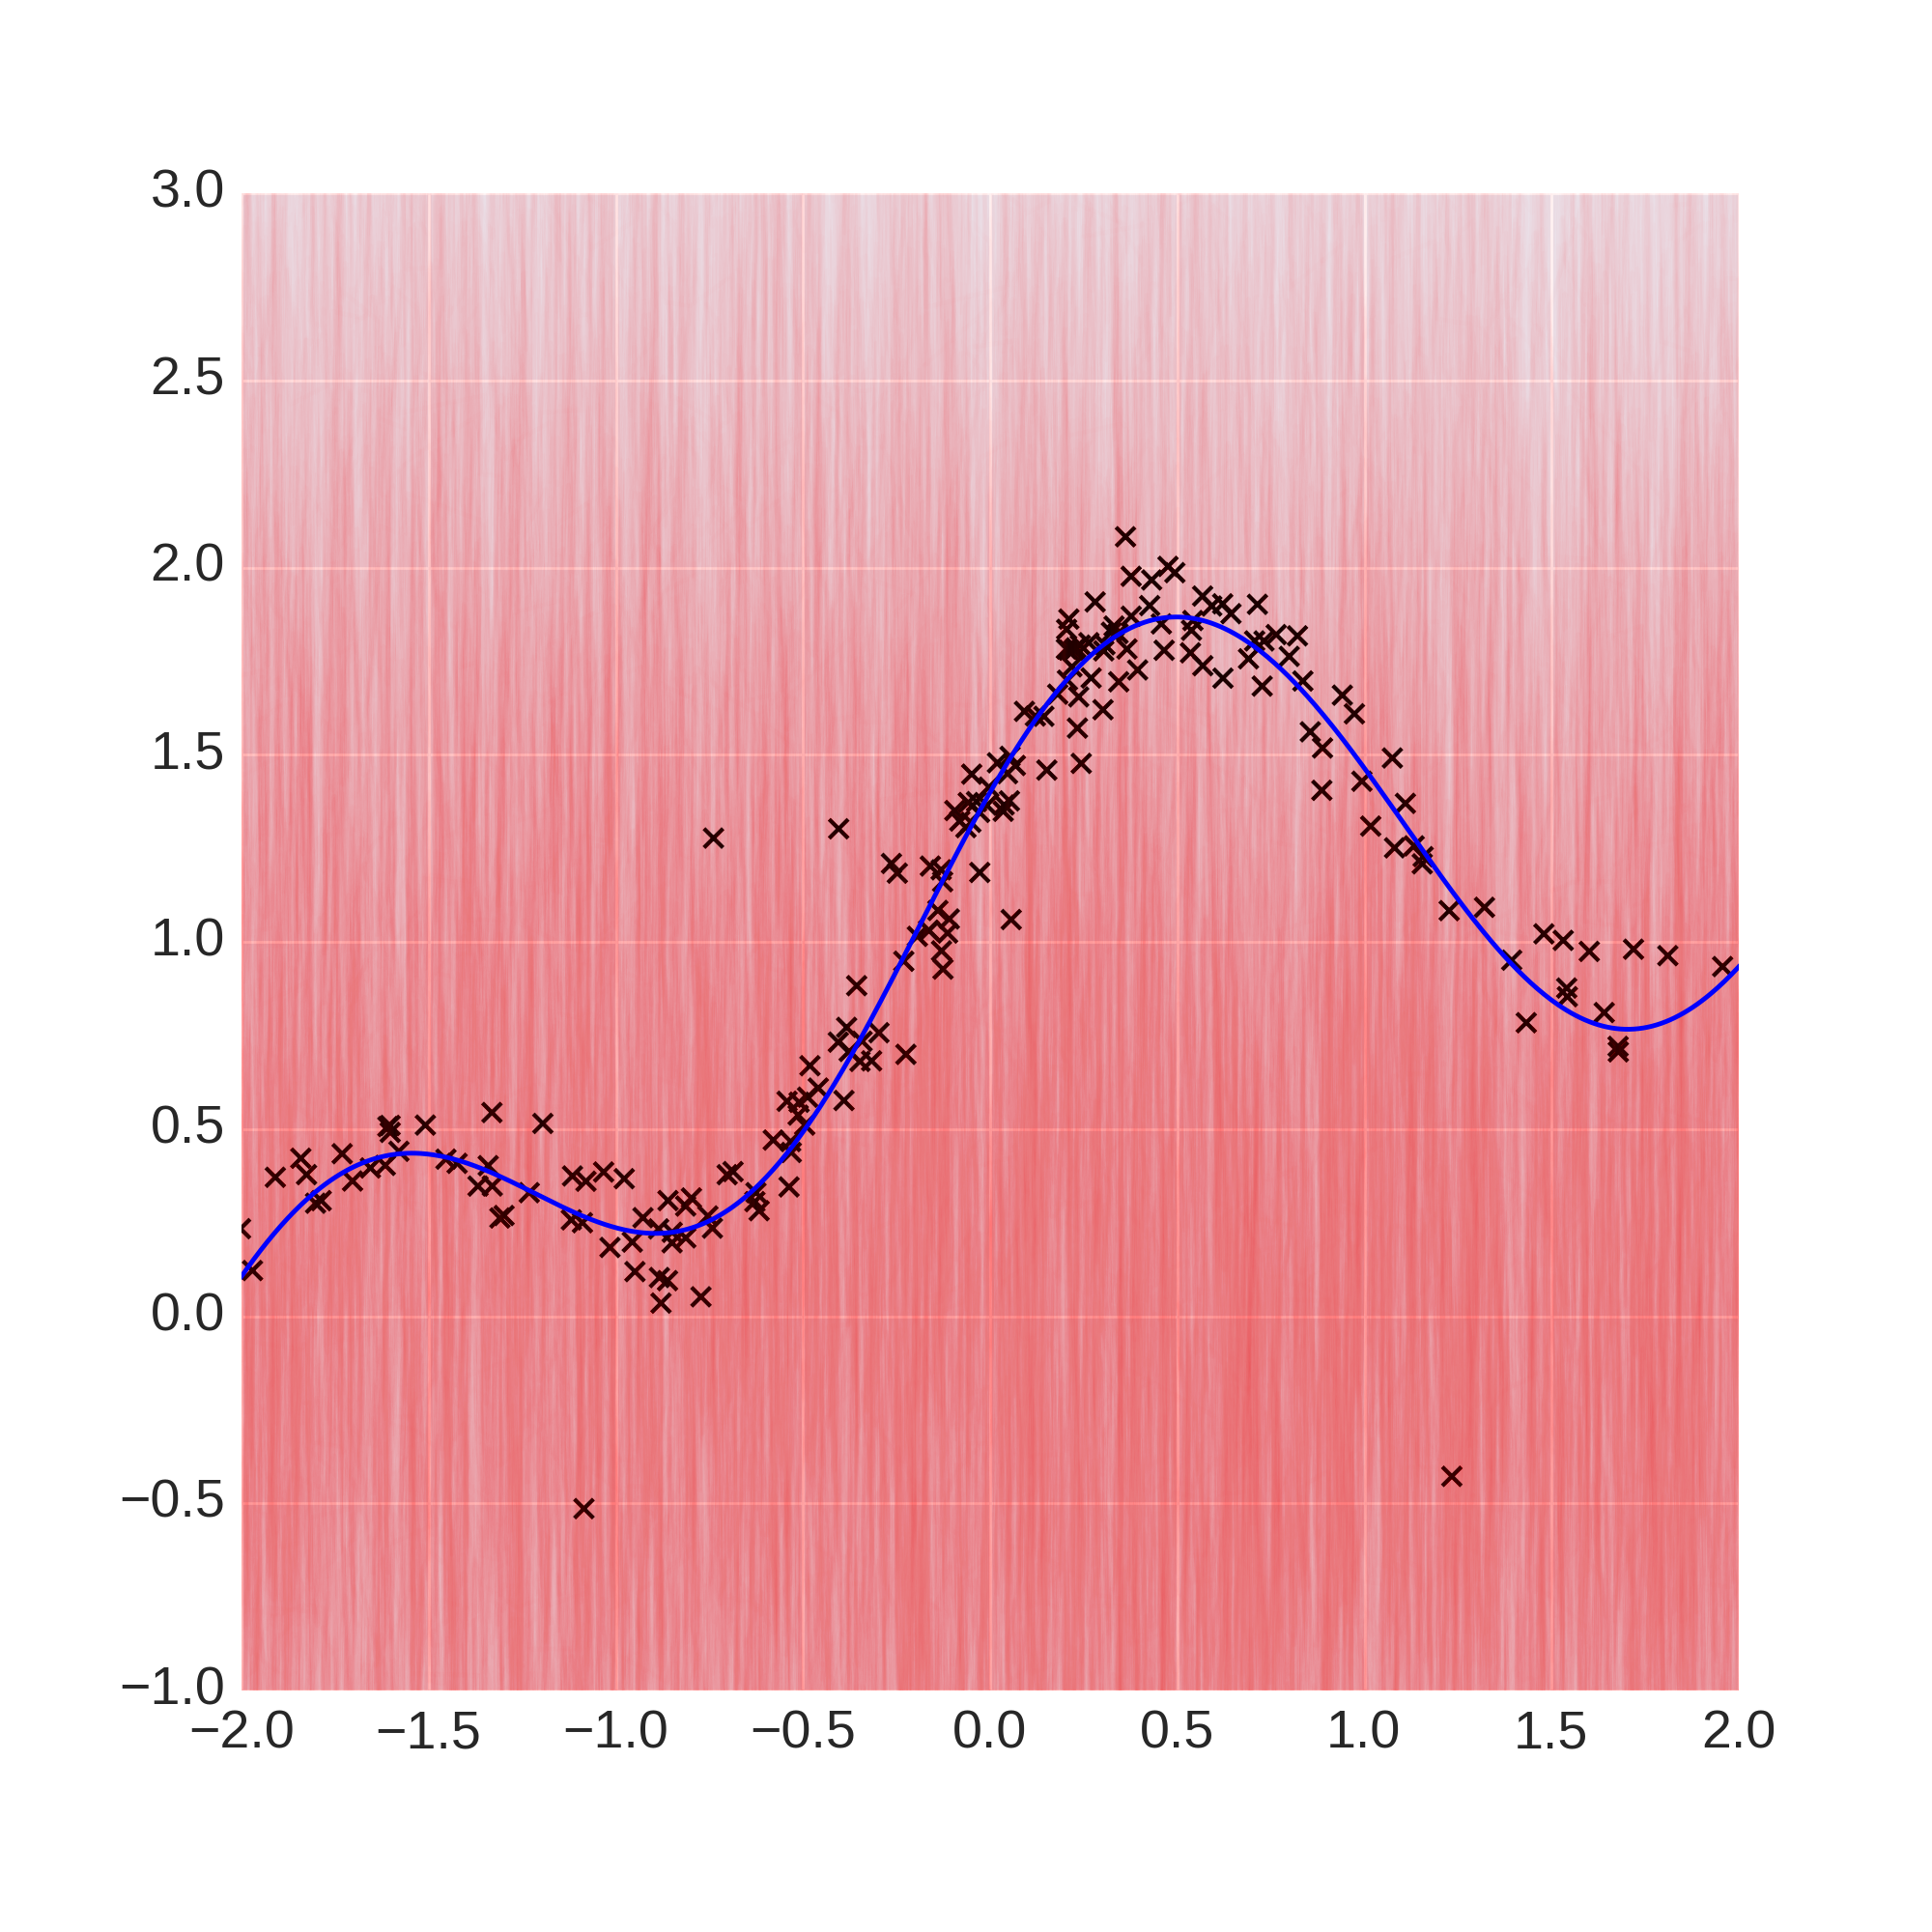
\includegraphics[height=7.5cm]{figs/neal_se_1final.png}
                \caption{Prior Inference}
                \label{fig:NealBO}
        \end{subfigure}%
        ~ %add desired spacing between images, e. g. ~, \quad, \qquad, \hfill etc.
          %(or a blank line to force the subfigure onto a new line)
        \begin{subfigure}[b]{0.49\textwidth} \centering
                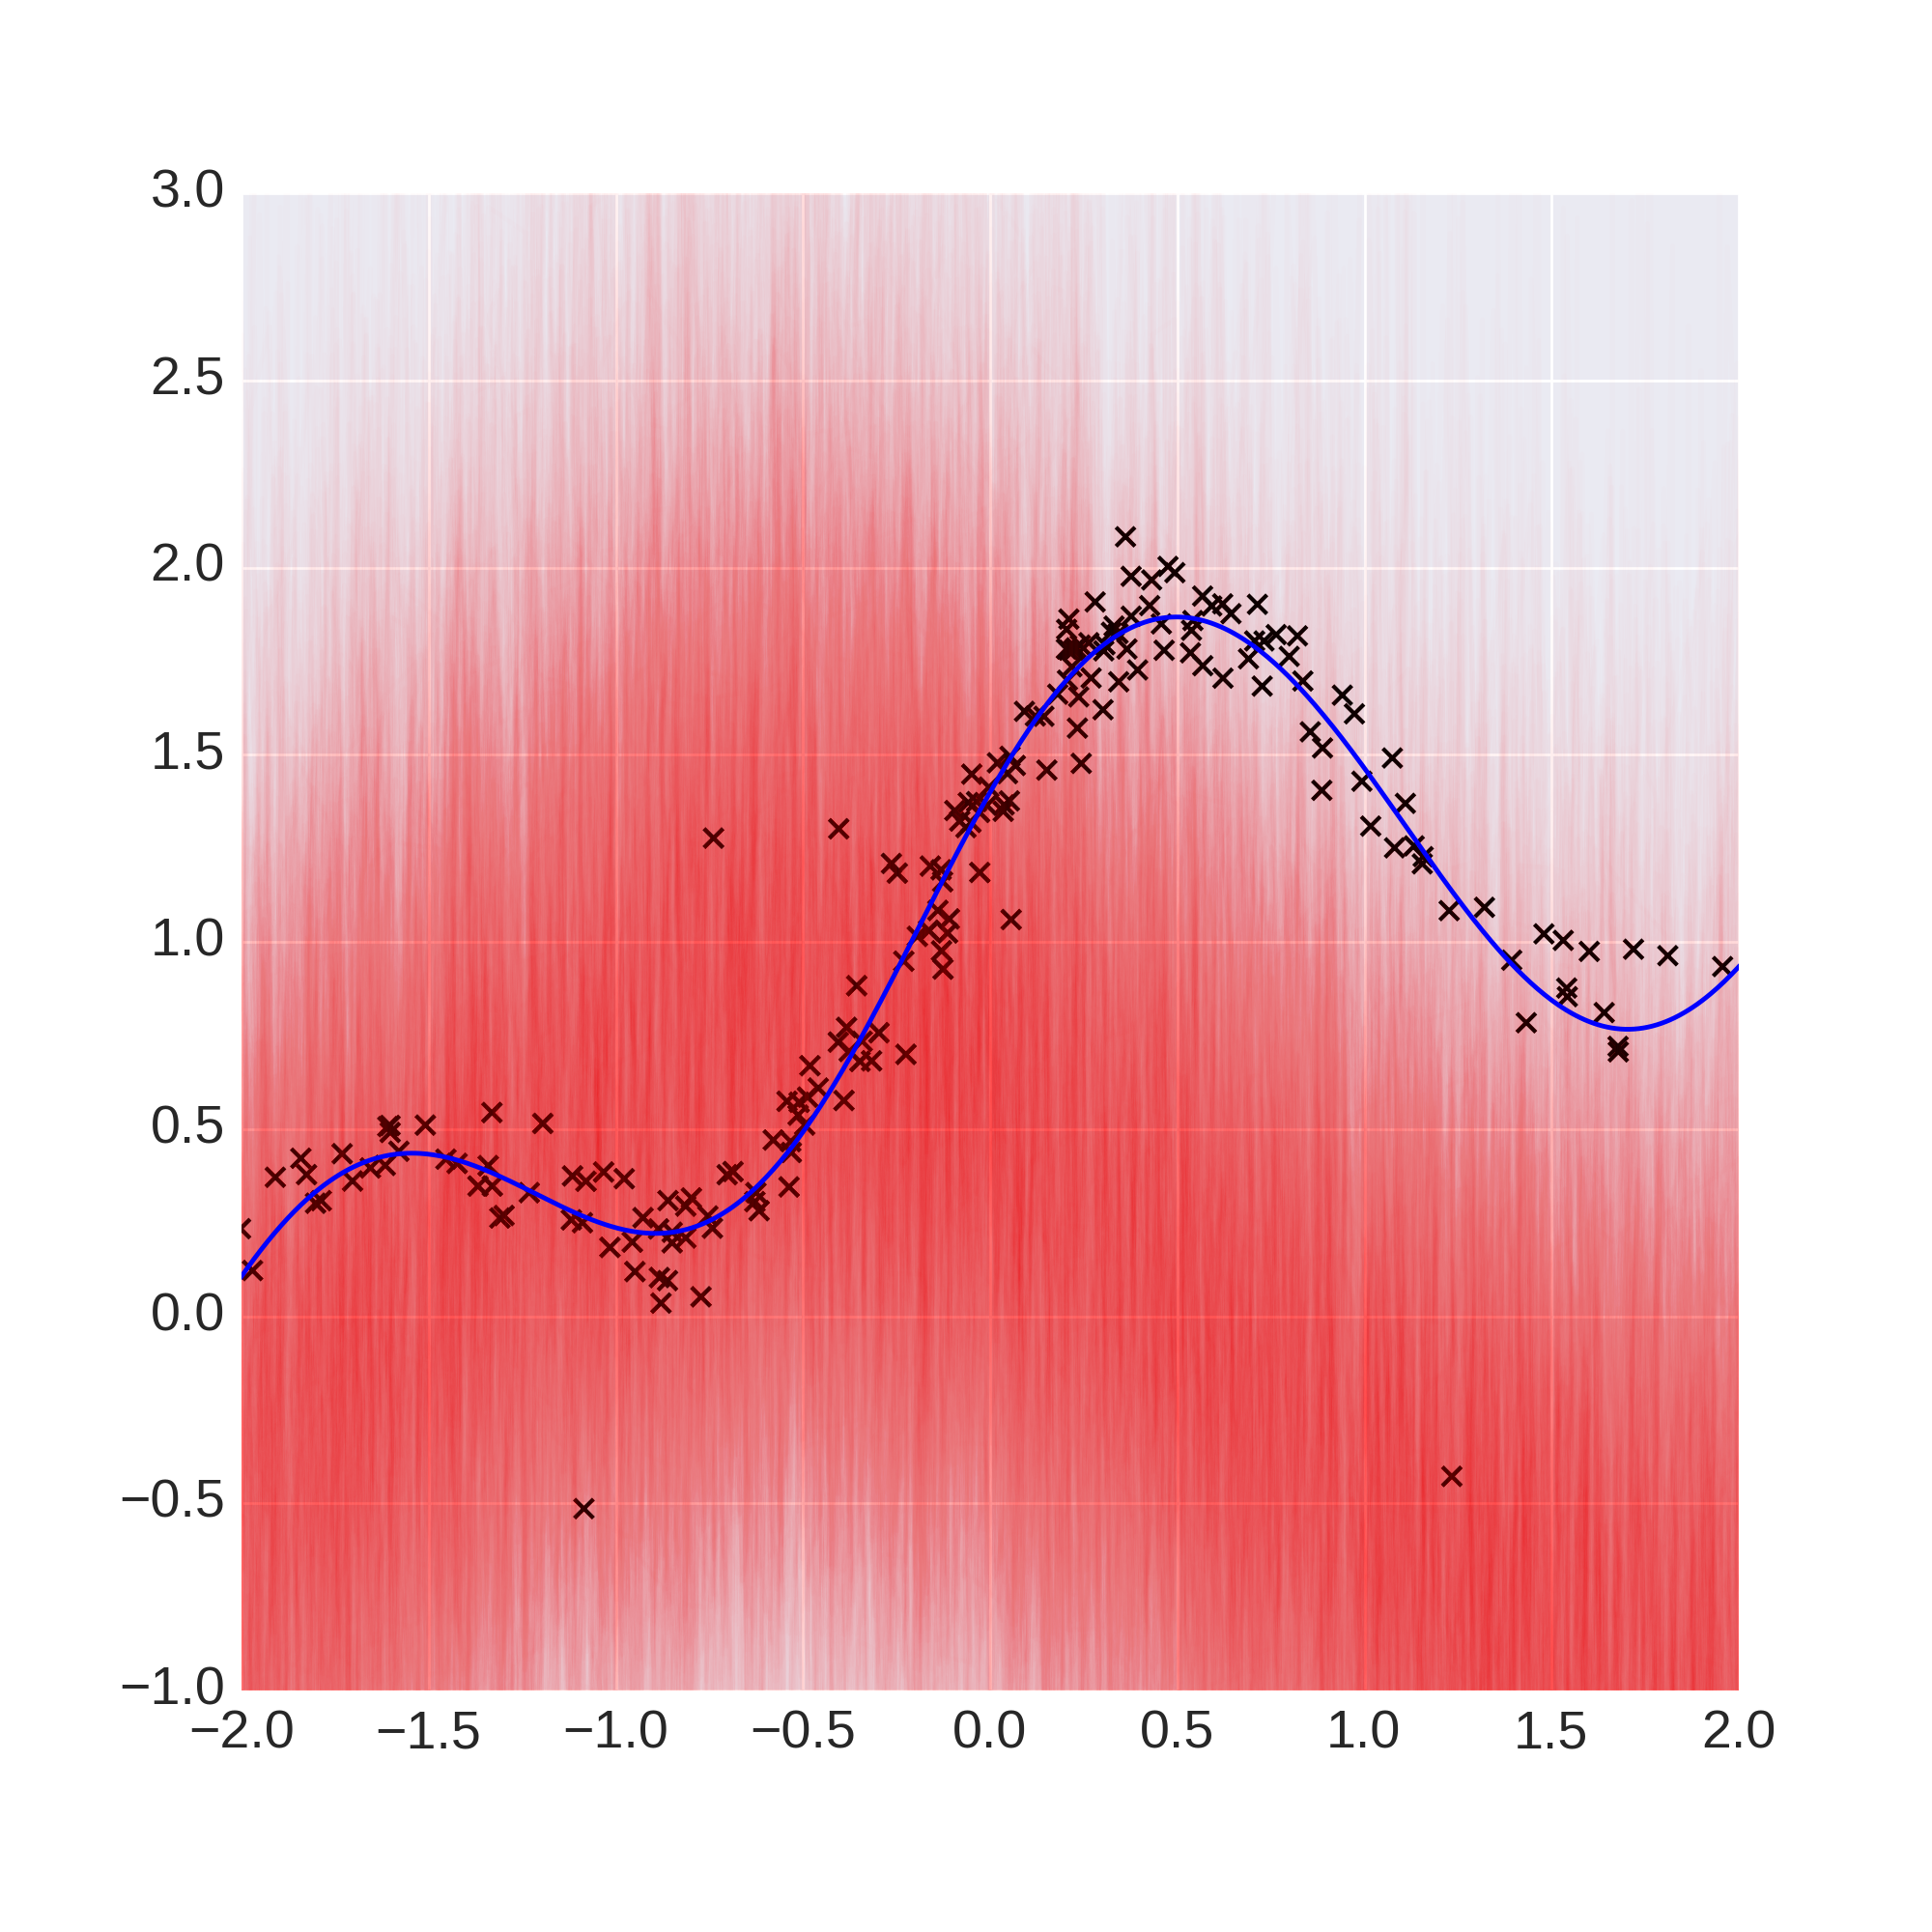
\includegraphics[height=7.5cm]{figs/neal_se_2final.png}
                \caption{Observed}
                \label{fig:NealAO}
        \end{subfigure}
        
        ~ %add desired spacing between images, e. g. ~, \quad, \qquad, \hfill etc.
          %(or a blank line to force the subfigure onto a new line)
        \begin{subfigure}[b]{0.49\textwidth} \centering
                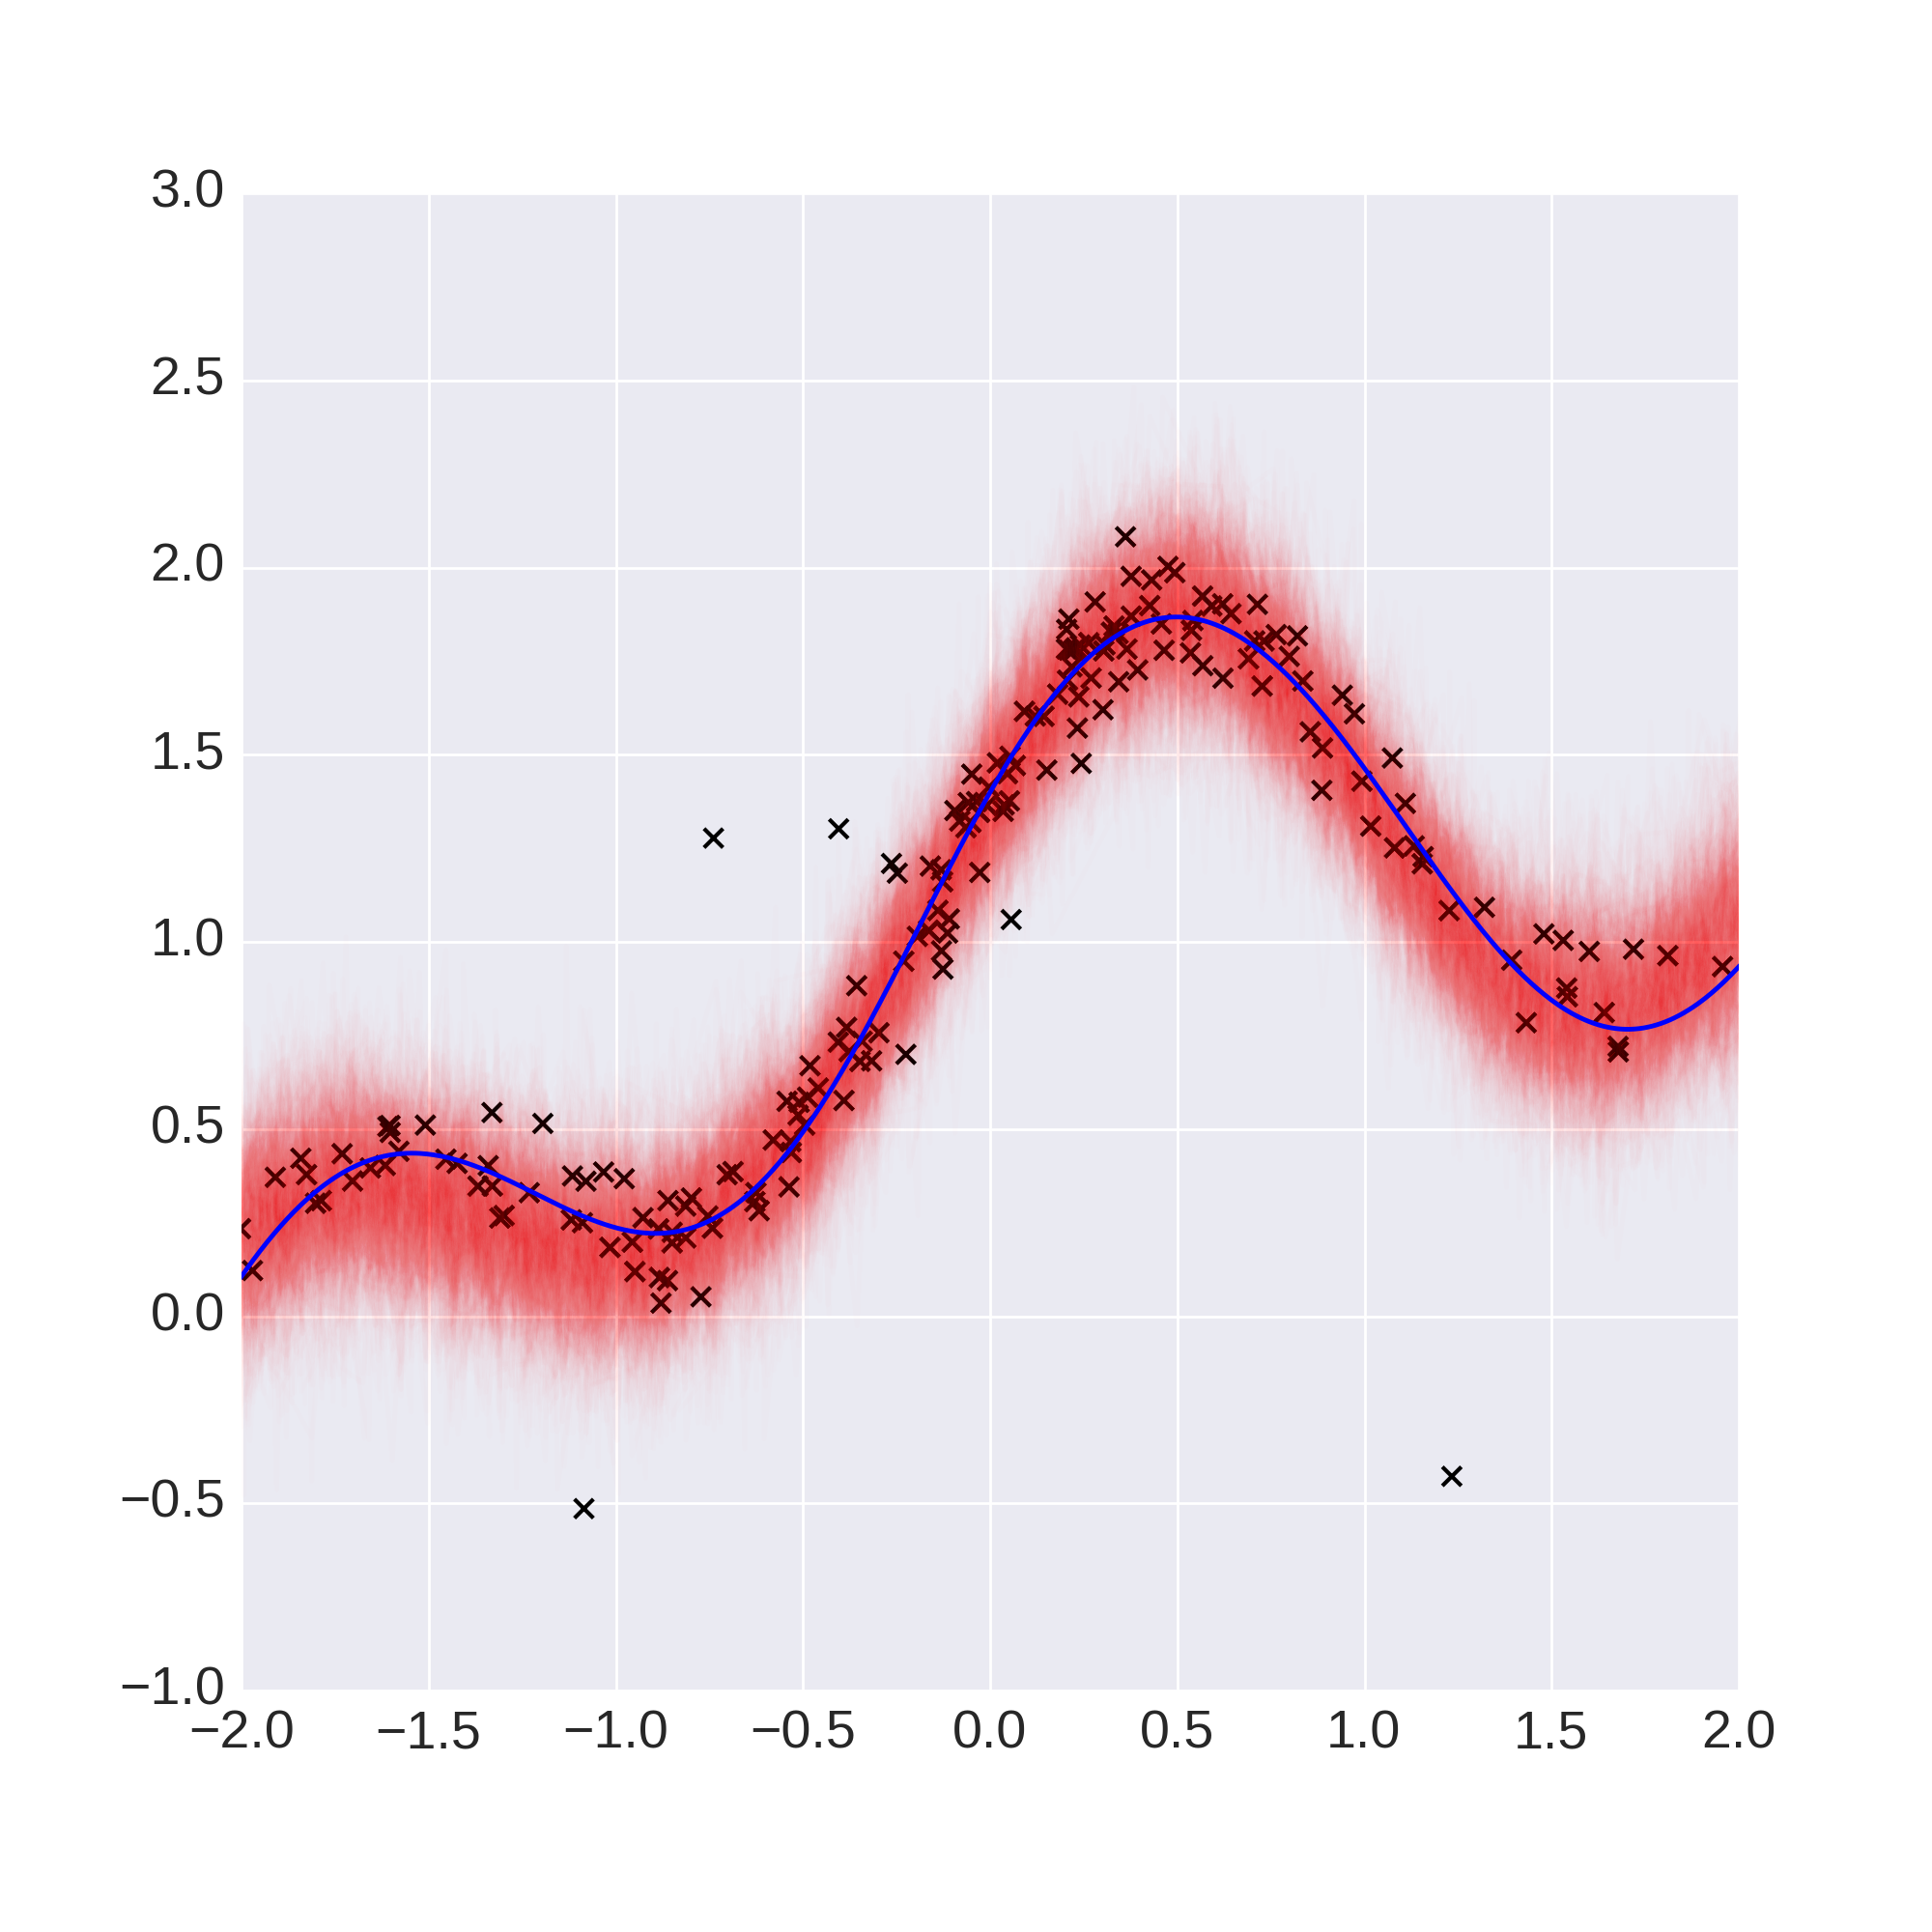
\includegraphics[height=7.5cm]{figs/neal_se_3final.png}
                \caption{Inferred}
                \label{fig:NealAI}
        \end{subfigure}
        \caption{(a)-(c) shows \gpmem\ on Neal's example. We see that prior renders functions all over the place (a). After \gpmem\ observes a some data-points an arbitrary smooth trend with a high level of noise is sampled. After running inference on the hierarchical system of hyper-parameters we see that the posterior reflects the actual curve well. Outliers are treated as such and do not confound the GP.}\label{fig:neal}
\end{figure}
We illustrate the hyper-parameter by showing the shift of the distribution on the noise parameter $\sigma$ (Fig. \ref{fig:inference}). We see that \gpmem\ learns the posterior distribution well, the posterior even exhibits a bimodal histogram when sampling $\sigma$ 100 times reflecting the two modes of data generation, that is normal noise and outliers\footnote{For this pedagogical example we have increased the probability for outliers in the data generation slightly from 0.05 to 0.2}. 

\begin{figure}
        \centering
        \begin{subfigure}[b]{0.5\textwidth} \centering
                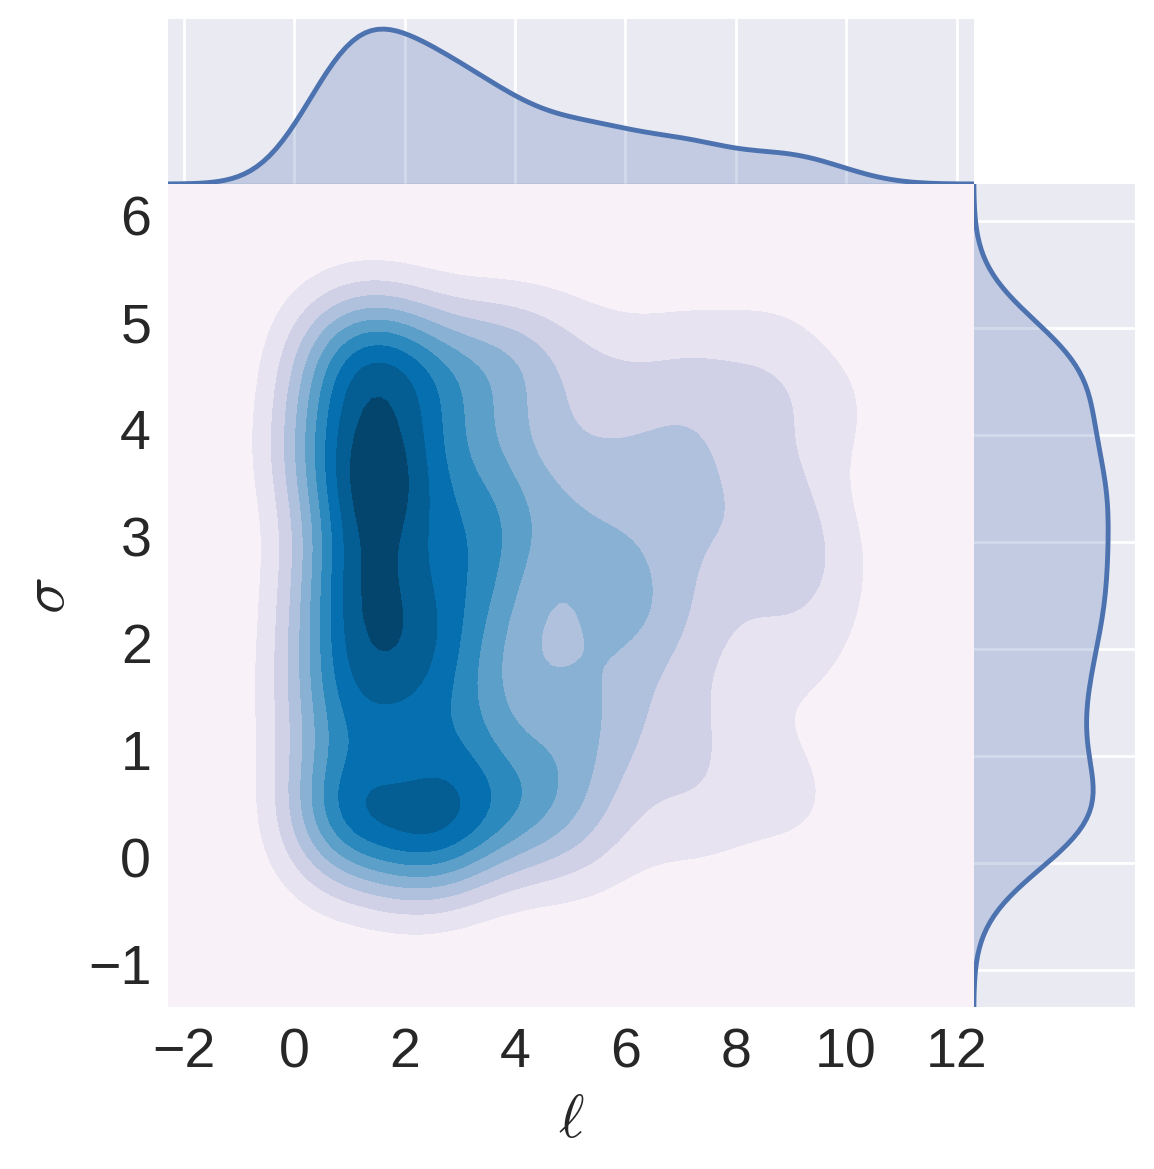
\includegraphics[height=6.5cm]{figs/neal_contour_l_vs_sigma_s__marginal_before.png}
                \caption{Before}
                \label{fig:before}
        \end{subfigure}%
        ~ %add desired spacing between images, e. g. ~, \quad, \qquad, \hfill etc.
          %(or a blank line to force the subfigure onto a new line)
        \begin{subfigure}[b]{0.5\textwidth} \centering
                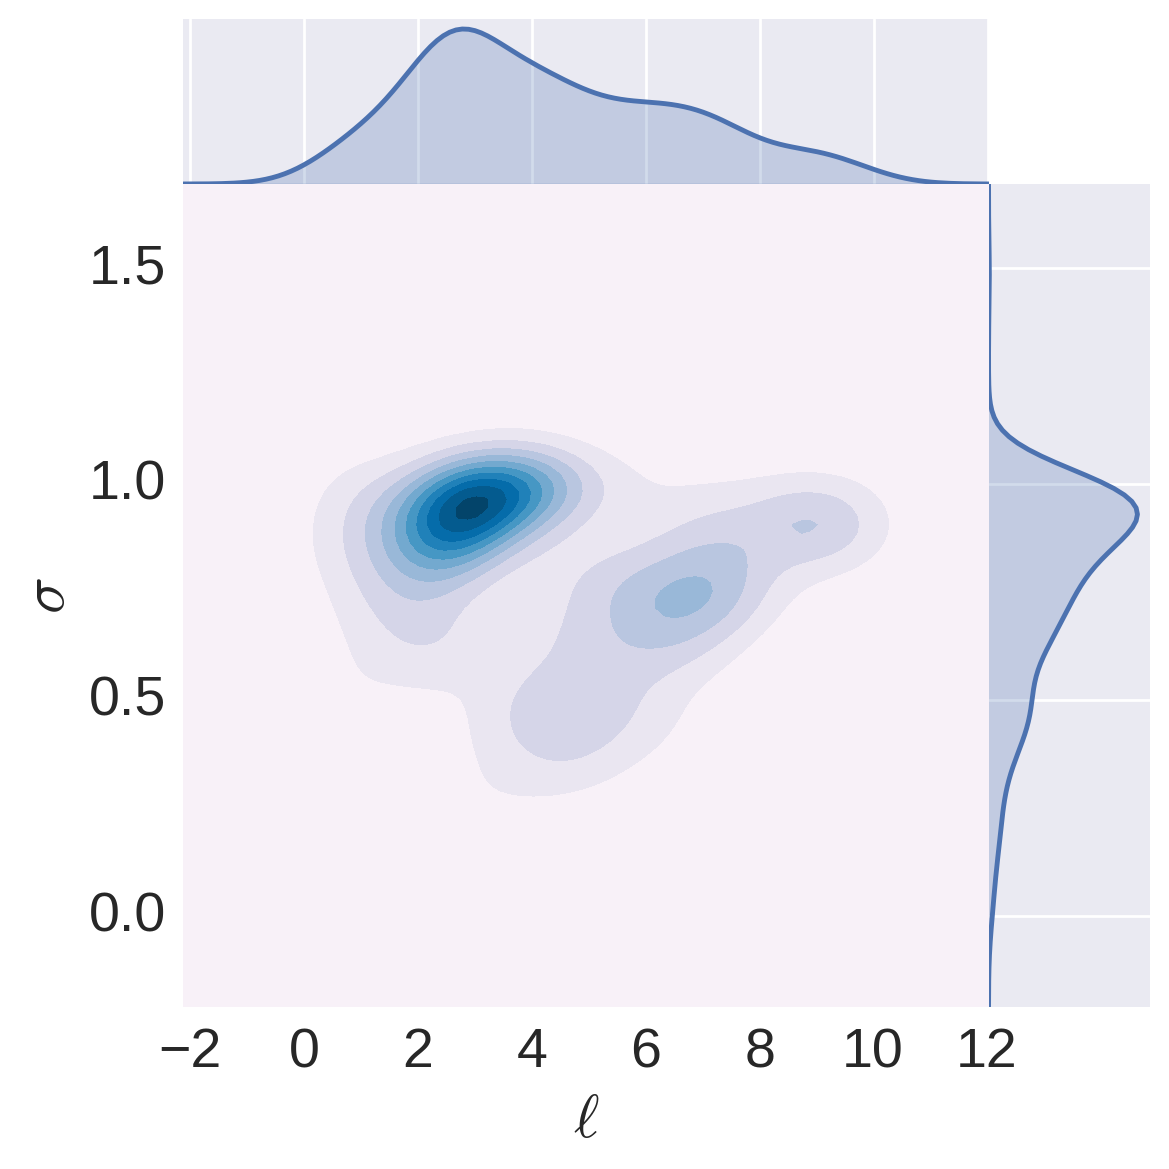
\includegraphics[height=6.5cm]{figs/neal_contour_l_vs_sigma_s__marginal_after.png}
                \caption{After}
                \label{fig:after))}
        \end{subfigure}
        \caption{Hyper-parameter inference on the parameter of the noise kernel. We show a 100 samples drawn from the distribution on $\sigma$. One can clearly recognise the shift from the uniform prior $\mathcal{U}(0,5)$ to a double peak distribution around the two modes - normal and outlier.}\label{fig:inference}
\end{figure}


%\subsubsection{Broader applicability of \gpmem}\label{sec:gpmem-broader}
%More generally, \gpmem\ is relevant not just when a data set is available, but also whenever we have at hand a function $f_\restr$ which is expensive or impractical to evaluate many times.
\gpmem\ allows us to model $f_\restr$ with a GP-based emulator $f_\emu$, and also to use $f_\emu$ during the learning process to choose, in an online manner, an effective set of probe points $\{x_i\}$ on which to use our few evaluations of $f_\restr$.
This idea is illustrated in detail in Section \ref{sec:bayesopt}.
Before doing this, we will illustrate another benefit of having a probabilistic programming apparatus for GP modelling: the linguistically unified treatment of inference over structure and inference over parameters.
This unification makes interleaved joint inference over structure and parameters very natural, and allows us to give a short, elegant description of what it means to ``learn the covariance function,'' both in prose and in code.
Furthermore, the example in Section \ref{sec:structurelearning} below recovers the performance of current state-of-the-art GP-based models.


\subsection{Discovering qualitative structure from time series data}\label{sec:structurelearning}
Inductive learning of symbolic expression for continuous-valued time series
data is a hard task which has recently been tackled using a greedy search over 
the approximate posterior of the possible kernel compostions for
\ac{GP}s~\citep{duvenaud2013structure,lloyd2014automatic}\footnote{\url{http://www.automaticstatistician.com/}}.

With \gpmem\ we can provide a fully Bayesian treatment of this, previously unavaible,
using a stochastic grammar  (see Fig. \ref{fig:schema}).

\begin{figure}
\centering
\usetikzlibrary{arrows, decorations.markings}
\usetikzlibrary{trees}

\tikzstyle{level 1}=[level distance=1cm, sibling distance=1.5cm]
\tikzstyle{level 2}=[level distance=1cm, sibling distance=1.1cm]

% Define styles for operators and leafs
\tikzstyle{operator} = [draw=none,circle, minimum width=1pt]
\tikzstyle{end} = [circle, minimum width=3pt,fill, inner sep=0pt]
% for double arrows a la chef
% adapt line thickness and line width, if needed

\begin{subfigure}[b]{0.49\textwidth}\centering
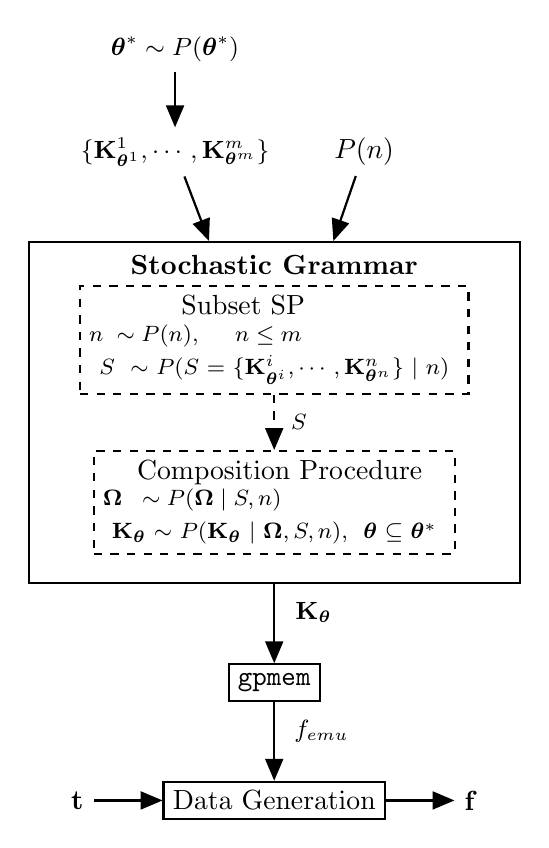
\begin{tikzpicture}[thick]
 \node[] (start) {};
 \node[left=-0.2cm of start] (base_kernels) {\small$\{\Kbf_{\bm{\theta}^1}^1,\cdots,\Kbf_{\bm{\theta}^m}^m\}$};
 \node[above=0.7cm of base_kernels] (theta) {\small$\bm{\theta}^* \sim P(\bm{\theta}^*)$};
\node[right=0.5cm of start] (n) {$P(n)$};
 \node[draw,rectangle, below=1cm of start, text width =6.0cm, text 
height=4.1cm,align=center] (grammar)
{};


 \node[draw,dashed,rectangle, below=-3.8cm of grammar, text width
=4.7cm,align=center] (subset) {
$\;\;\;\;\;\;\;\;\;\;\;\;$Subset SP % I can't believe that this is the simpliest way to
% get spacing right 
{\raggedright
\footnotesize$ n\; \sim P(n),\;\;\;\;\; n \leq m$ \\

\footnotesize$S \; \sim P(S = \{\Kbf_{\bm{\theta}^i}^i,\cdots,\Kbf_{\bm{\theta}^n}^n\} \mid n)$
}
};
 \node[draw,rectangle,dashed, below=0.7cm of subset, text width
=4.35cm,align=center]
(composition_procedure) {
$\;$Composition Procedure\\ % I can't believe that this is the simpliest way to
% get spacing right 
{\raggedright
\footnotesize$\bm{\Omega}\;\; \sim P(\bm{\Omega} \mid S,n)$ \\

\footnotesize$\Kbf_{\bm{\theta}} \sim P(\Kbf_{\bm{\theta}} \mid \bm{\Omega},S,n),\;\,\bm{\theta}\subseteq\bm{\theta}^*$
}
};

\node[above=0.0cm of subset]{\centering \bf Stochastic Grammar}; 

 \node[draw,rectangle,below=1cm of grammar] (gpmem) {\texttt{gpmem}};

 \node[draw,rectangle,below=1cm of gpmem] (f) {Data Generation};
\node[left of=f,xshift=-1.5cm] (x) {$\mathbf{t}$};
\node[right of=f,xshift=1.5cm] (y) {$\mathbf{f}$};

 \node[below=0.1cm  of grammar,xshift=0.5cm] (k)
{\small$\Kbf_{\bm{\theta}}$};


\node[below=0.1cm  of gpmem,xshift=0.6cm] (gp) {
\small$f_{emu}$};

% 1st pass: draw arrows
  \draw[thick,->] (base_kernels) -- (grammar);
  \draw[thick,->] (n) -- (grammar);
  \draw[thick,->] (theta) -- (base_kernels);
  \draw[thick,->] (grammar) -- (gpmem);
  \draw[thick,->] (gpmem) -- (f);
 \draw[thick,->] (x) -- (f);
 \draw[thick,->] (f) -- (y);
 \draw[thick,dashed,->] (subset) -- node[right]{\footnotesize $\;S$} (composition_procedure);
  % Note: If you have no branches, the 2nd pass is not needed
\end{tikzpicture}\vspace{2mm}
\caption{} 
\end{subfigure}
\begin{subfigure}[b]{0.49\textwidth}\centering
\begin{tikzpicture}[grow=right, sloped]
\node[operator] {\small $+$}
    child {
        node[operator] {\small $+$}        
            child {
               node[operator] {\small $\times$}        
        child {
                node[operator, label=right:
                    {$\cdots$}] {}
                edge from parent
                node[above] {}
                node[below]  {}
            }
            child {
                node[end, label=right:
                    {SE$_{\theta^4}$}] {}
                edge from parent
                node[above] {}
                node[below]  {}
            }
        edge from parent         
            node[above] {}
            node[below]  {}
            }
            child {
                node[end, label=right:
                    {WN$_{\theta^3}$}] {}
                edge from parent
                node[above] {}
                node[below]  {}
            }
            edge from parent 
            node[above] {}
            node[below]  {}
    }
    child {
        node[operator] {\small $\times$}        
        child {
                node[end, label=right:
                    {PER$_{\theta^2}$}] {}
                edge from parent
                node[above] {}
                node[below]  {}
            }
            child {
                node[end, label=right:
                    {LIN$_{\theta^1}$}] {}
                edge from parent
                node[above] {}
                node[below]  {}
            }
        edge from parent         
            node[above] {}
            node[below]  {}
    };
\node[xshift=-0.7cm] (K) {$\mathbf{K}_{\bm{\theta}}=$}; 
 \node[xshift=2.6cm,below =2.4cm of K] (Keq) {$\mathbf{K}_{\bm{\theta}}=\text{LIN}_{\theta^1} \times \text{PER}_{\theta^2}+\text{WN}_{\theta^3} + \text{SE}_{\theta^4} \times ( \cdots )$};
\end{tikzpicture}
\caption{} 
\end{subfigure}

\begin{subfigure}[b]{0.99\textwidth}\centering
\begin{tabular}{cccc}
\multicolumn{4}{c}{\bf Base Components} \rule{0pt}{3ex} \\ 
\small LIN: Linearity &\small PER: Periodicity &\small SE: Smoothness &\small WN: White Noise \rule{0pt}{2ex} \\
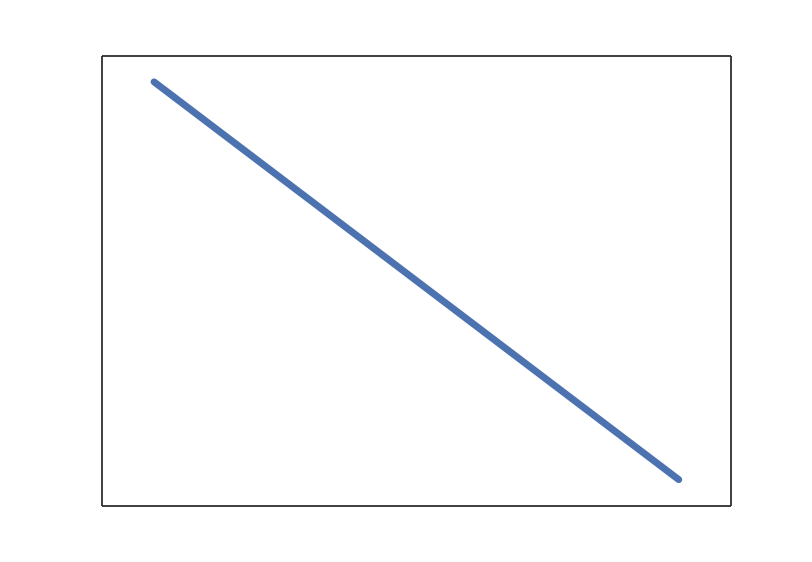
\includegraphics[height=2cm]{figs/kernel/kernelLIN.png} & 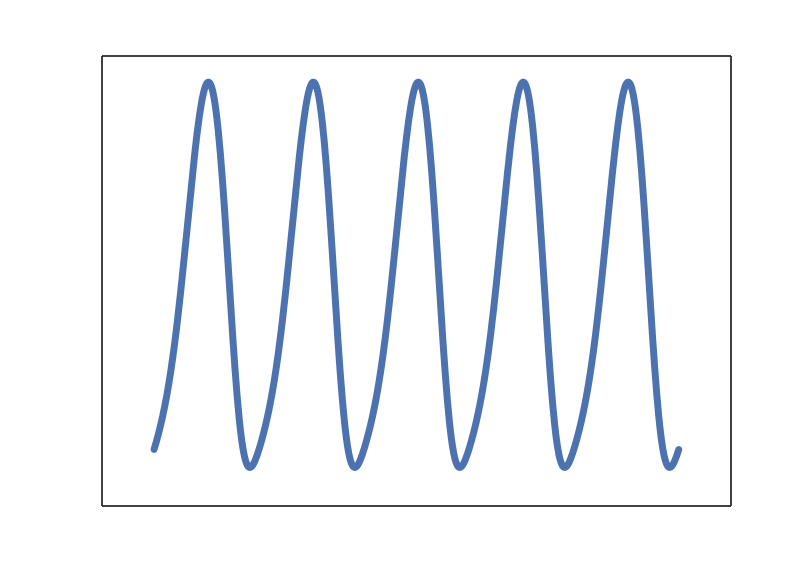
\includegraphics[height=2cm]{figs/kernel/kernelPER.png} & 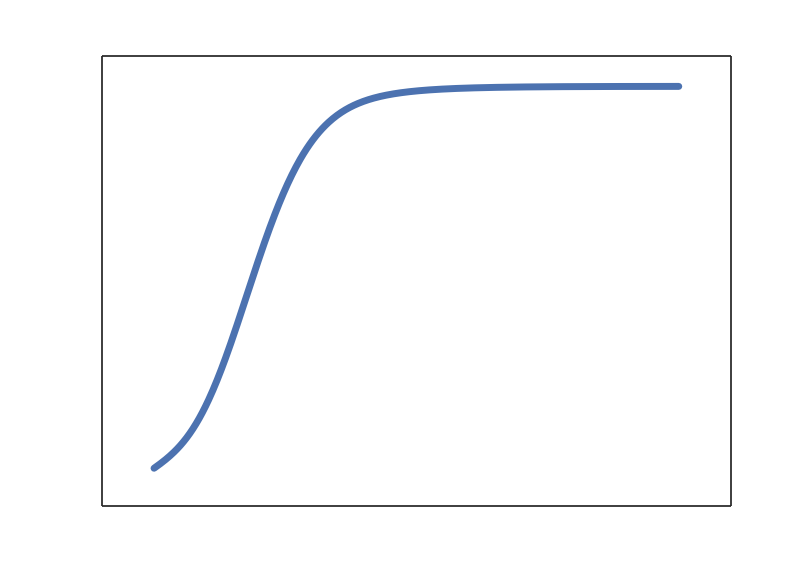
\includegraphics[height=2cm]{figs/kernel/kernelSE.png} & 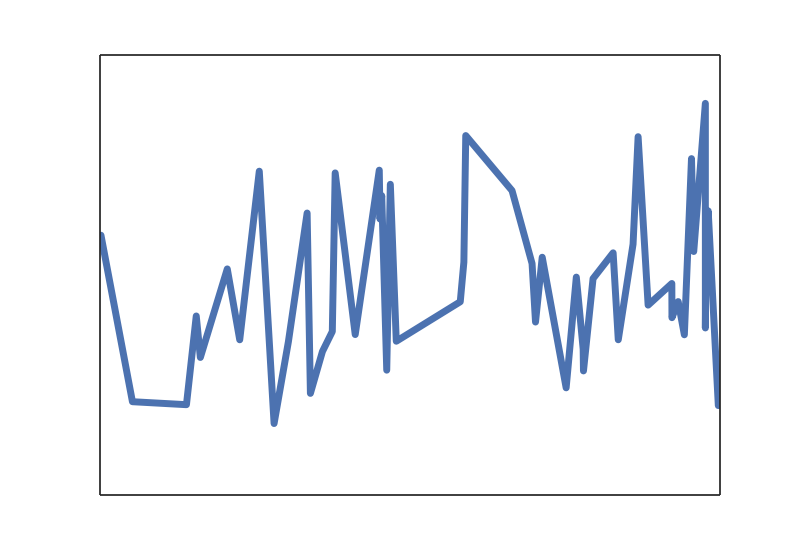
\includegraphics[height=2cm]{figs/kernel/kernelWN.png}\\
\end{tabular}
\begin{tabular}{cccc}
\multicolumn{4}{c}{\bf Composite Structure} \rule{0pt}{0ex}  \\ 
\small LIN + PER: &\small LIN $\times$ PER: &\small SE $\times$ PER: &\small LIN $\times$ LIN: \rule{0pt}{2ex} \\
\small Periodicity with Trend &\small Growing Amplitude &\small Local Periodicity&\small Quadratic \rule{0pt}{2ex} \\
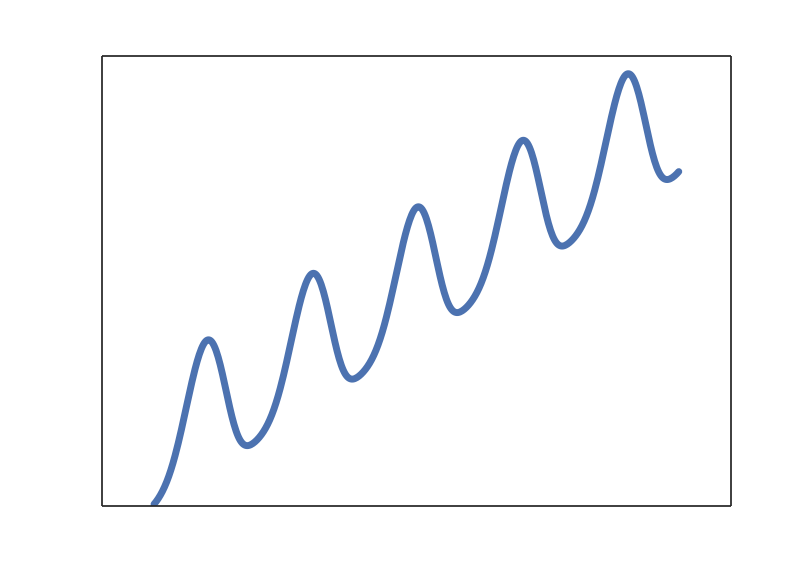
\includegraphics[height=2cm]{figs/kernel/kernelLINplusPER.png} & 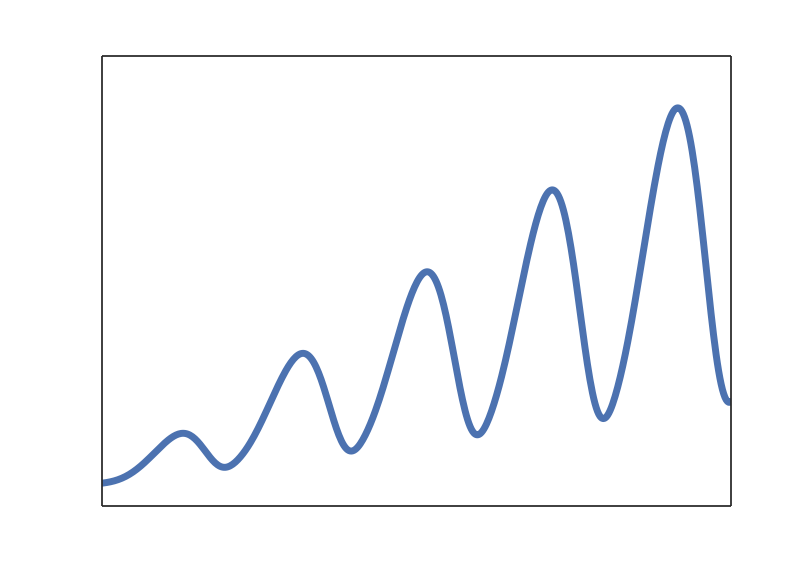
\includegraphics[height=2cm]{figs/kernel/kernelLINtimesPER.png} & 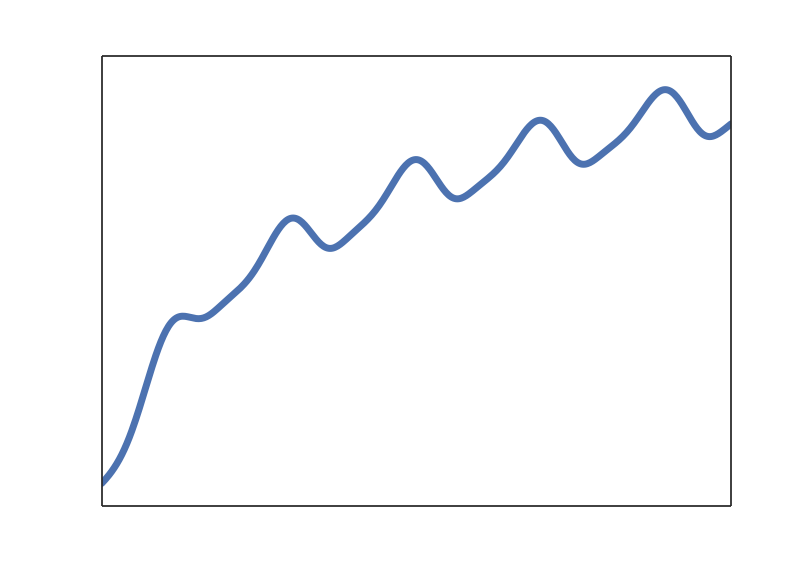
\includegraphics[height=2cm]{figs/kernel/kernelSEplusPER.png}& 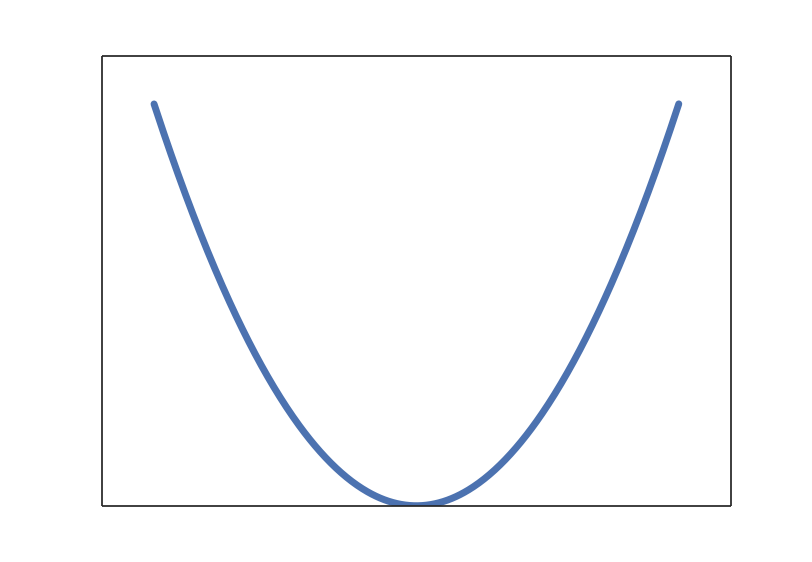
\includegraphics[height=2cm]{figs/kernel/kernelLINtimesLIN.png}\\
\end{tabular}
\caption{}
\end{subfigure}

\caption{(a) Graphical description of Bayesian GP structure learning. (b) Composite structure. (c) The natural language interpretation of the structure.}\label{fig:schema}
\end{figure}

The stochastic grammar models a prior on different structural compositions of the covariance function. An input of non-composite kernels (base kernels) is supplied to generate a posterior distributions of composite structure to express local and global aspects of the data.


We approximate the following intractable integrals of the expectation for the prediction:
\begin{equation}
\mathbb{E}[\hat{f} \mid \hat{x},\mathbf{D},\mathbf{K}] =\iint f(\hat{x},\bm{\theta},\mathbf{K})\,P(\bm{\theta} \mid \mathbf{D,\mathbf{K}})\,P(\mathbf{K}|\bm{\Omega},s,n) \; \mathbf{d} \bm{\theta} \mathbf{d} \mathbf{K}.  
\end{equation}

This is done by sampling from the posterior probability distribution of the hyper-parameters and the possible kernel:
\begin{equation}
\hat{f} \approx \frac{1}{T} \sum^T_{t=1} f(\hat{x} | \bm{\theta}^{(t)},\mathbf{K}^{(t)}). 
\end{equation}


In order to provide the sampling of the kernel, we introduce a stochastic process that simulates the grammar for algebraic expressions of covariance function algebra:
\begin{equation}
\mathbf{K}^{(t)} \sim  P(\mathbf{K} \mid \bm{\Omega},s,n)
\end{equation}
Here, we start with the set of given base kernels and draw a random subset.
For this subset of size $n$, we sample a set of possible operators $\bm{\Omega}$ combining base kernels. 
The marginal probability of a composite structure
\begin{equation}
P(\mathbf{K} \mid \bm{\Omega},s,n) = P(\bm{\Omega} \mid s,n)\times P(s \mid n) \times P(n),
\end{equation}
is characterized by the prior $P(n)$ on the number of base kernels used, the probability of a uniformly chosen subset of the set of $n$ possible covariance functions
\begin{equation}
\label{eq:subsets}
P(s \mid n) = \frac{n!}{ \mid s \mid !},
\end{equation}
and the probability of sampling a global or a local structure, which is given by a binomial distribution: 
\begin{equation}
P(\bm{\Omega} \mid s,n)= {n \choose r}  p_{+\times}^r (1 - p_{+\times})^{n-r}.
\end{equation}



Many equivalent covariance structures can be sampled due to covariance function algebra and equivalent representations with different parameterization~\citep{lloyd2014automatic}. To inspect the posterior of these equivalent structures we convert each kernel expression into a sum of products and subsequently simplify. All base kernels can be found in Appendix A, rules for this simplification can be found in appendix B. The code for learning of kernel structure is as follows:

\begin{mdframed}
\begin{minipage}{\linewidth}
\small
\belowcaptionskip=-10pt
\begin{lstlisting}[mathescape,label=alg:structureVent,basicstyle=\selectfont\ttfamily,numbers=none,escapechar=\#]
// GRAMMAR FOR KERNEL STRUCTURE
#\linenumber{1}#assume kernels = list(se, wn, lin, per, rq) // defined as above

// prior on the number of kernels
#\linenumber{2}#assume p_number_k = uniform_structure(n)
#\linenumber{3}#assume subset_kernels = tag(quote(grammar), 0,
#\linenumber{4}#                            subset(kernels, p_number_k))

// kernel composition
#\linenumber{5}#assume composition = proc(l) {
#\linenumber{6}#  if (size(l) <= 1) {
#\linenumber{7}#    first(l)
#\linenumber{8}#  } else {
#\linenumber{9}#    if (bernoulli()) {
#\linenumber{10}#      add_funcs(first(l), composition(rest(l)))
#\linenumber{11}#    } else {
#\linenumber{12}#       mult_funcs(first(l), composition(rest(l)))
#\linenumber{13}#    }
#\linenumber{14}#  }
#\linenumber{15}#}

#\linenumber{16}#assume K = tag(quote(grammar), 1, composition(subset_kernels))

// APPLY GPMEM
#\linenumber{17}#assume (f_compute, f_emu) = gpmem(f_look_up, K)

// Probe all data points
#\linenumber{18}#for n ... N
#\linenumber{19}#  predict f_compute(get_data_xs(n))

// PERFORMING INFERENCE
#\linenumber{20}#infer repeat(200, do(
#\linenumber{21}#  mh(quote(grammar), one, 1),
#\linenumber{22}#  for kernel in K:
#\linenumber{23}#    mh(quote(parameters$_{\text{kernel}}$), one, 1)))
\end{lstlisting}

\end{minipage}
\end{mdframed}


We defined a simmple space of covariance structures in a way that allows us to produce results coherent with 
work presented in Automatic Statistician. We illustrate results in Fig. \ref{fig:posterior} and \ref{fig:posterior_airline} using the Mauna Loa  CO$_2$ data set (see \citealp{rasmussen2006gaussian} for a description) and the airline data set describing monthly totals of international airline passengers (\citealp{box2011time}, according to \citealp{duvenaud2013structure}). Both datasets served as illustration in the Automatic Statistician project. Previous work on automated kernel discovery~\citep{duvenaud2013structure} illustrated the Mauna Loa data using an RQ kernel.
We resort to the white noise kernel instead RQ (similar to \citep{lloyd2014automatic}).

In contrast to what previous work has presented, we compute a posterior on structures. This allows us to gain valuable insight into the data that was previously unavailable. 
We can query the data for the probability of certain structures to hold true. For example, we could be interested in whether or not a trend as is present in the data.
We can also formulate queries using logical operators such as AND and OR. This provides us with a rich language to ask questions about our time series data and let the data speak for itself for finding the answers. We demonstrate this in Fig \ref{fig:query}.

\begin{figure}
\centering
 \addtolength\abovedisplayskip{-1\baselineskip}%
  \addtolength\belowdisplayskip{-1\baselineskip}%
 
\begin{tikzpicture}
\node (datatitle) {\small Raw Data};
\node[below = -0.25cm of datatitle] (data) {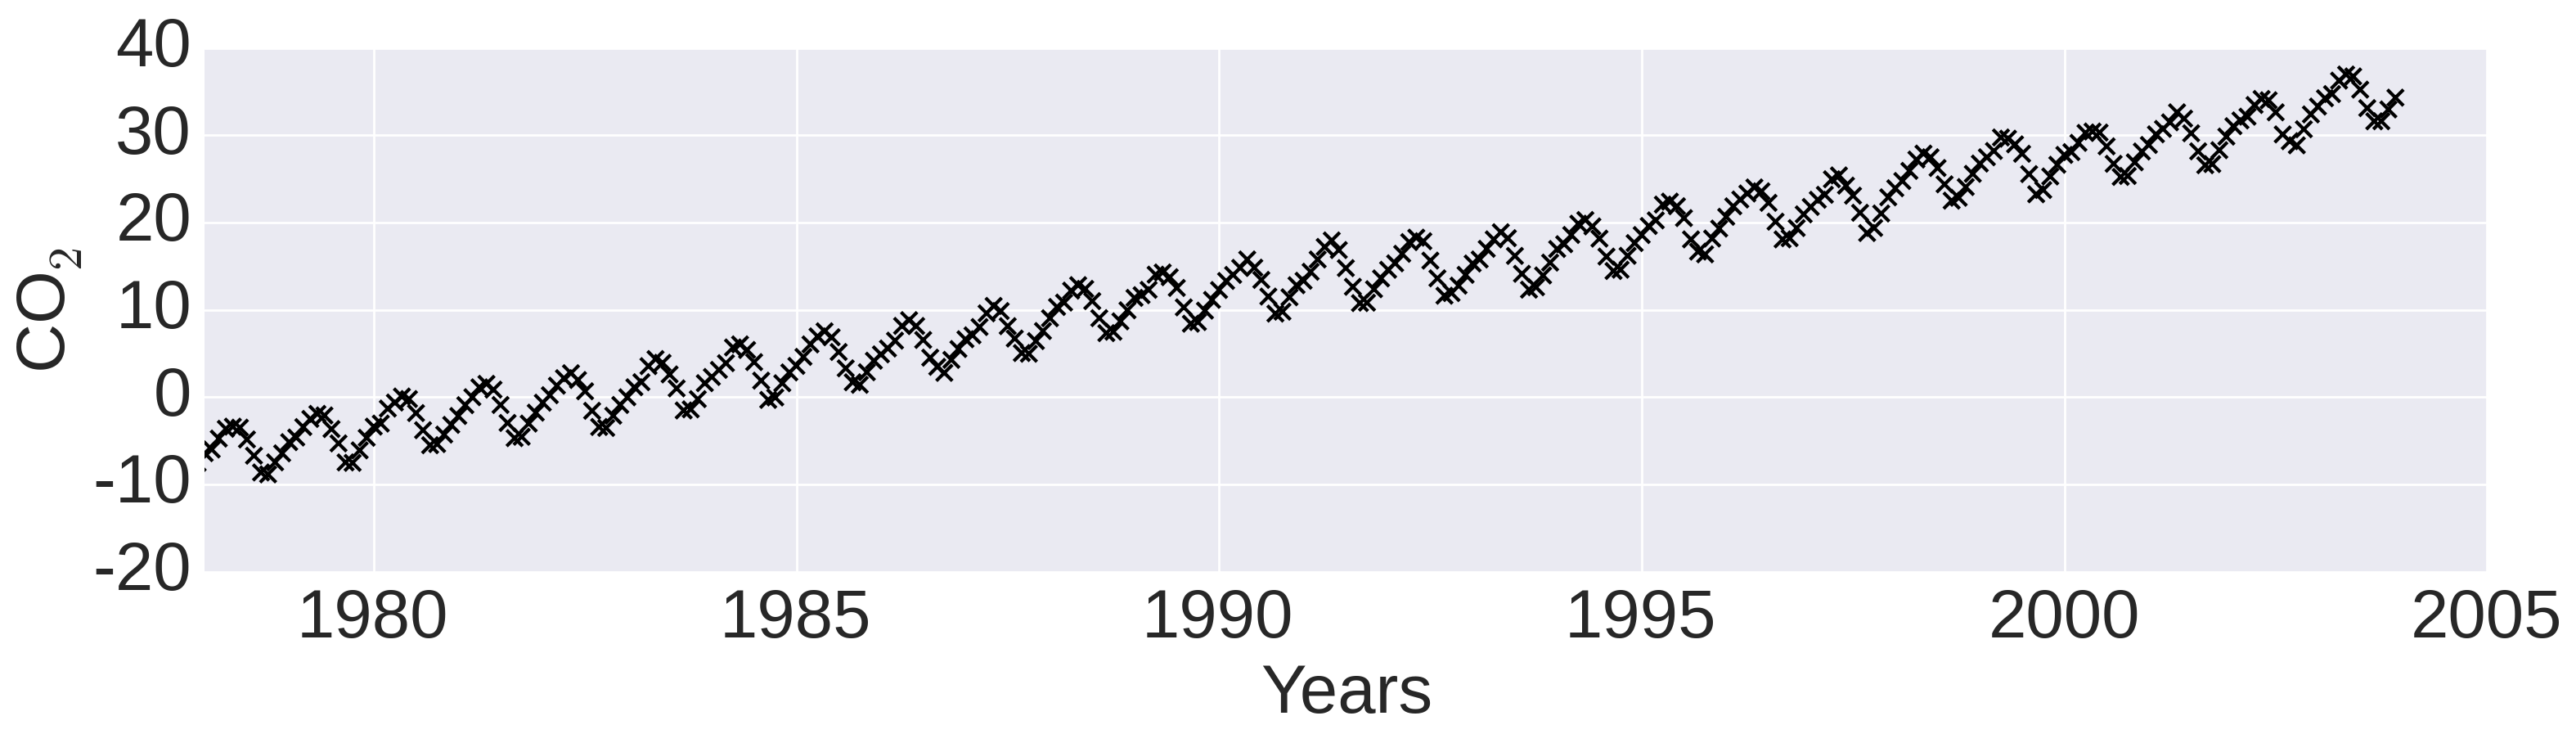
\includegraphics[width=0.7\textwidth]{figs/mauna_data.png}};
\node[below = 2.5cm of data] (post_param_helper) {};
\node[above = 1cm of post_param_helper] (post_param_helper_1) {};
\node[below = 1cm of post_param_helper] (post_param_helper_2) {};
\node[left = -3cm of post_param_helper] (post_param) {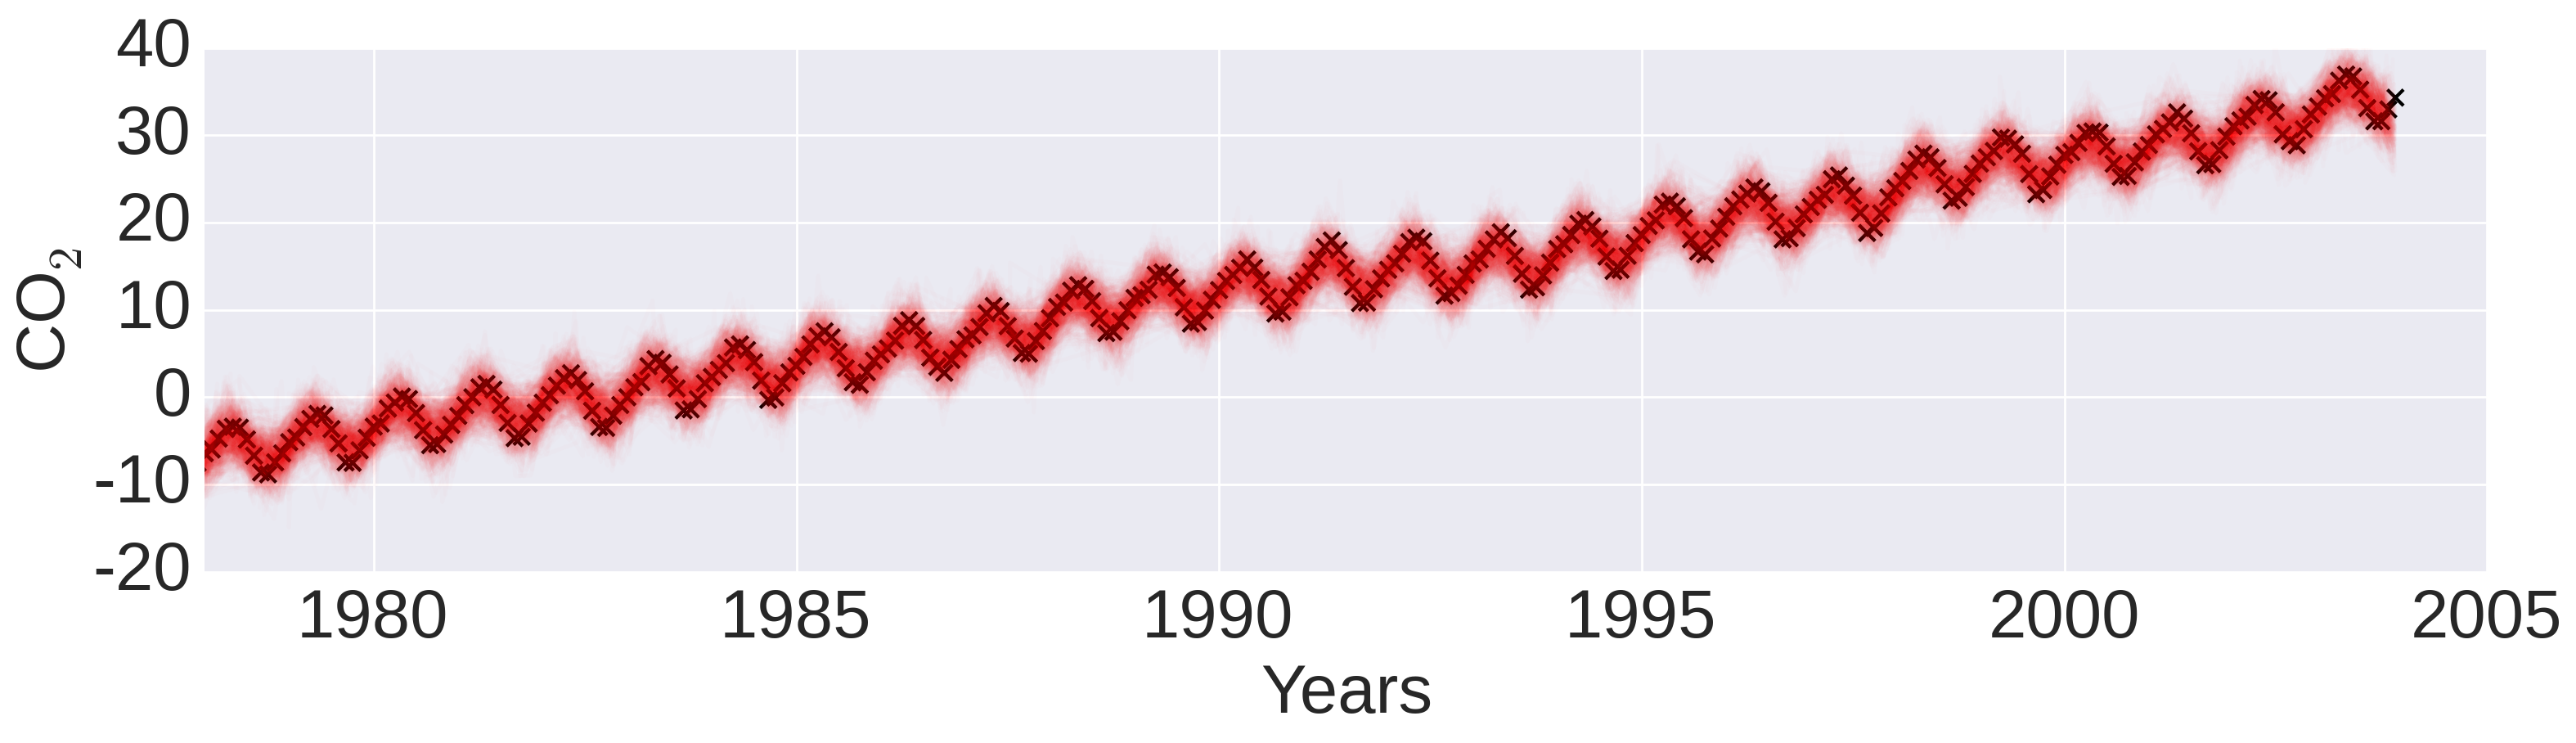
\includegraphics[width=0.6\textwidth]{figs/mauna_sample_1.png}};
\node[draw,rectangle,color=red,dashed,right = 4.5cm of post_param_helper,yshift=0.3cm] (zoom) {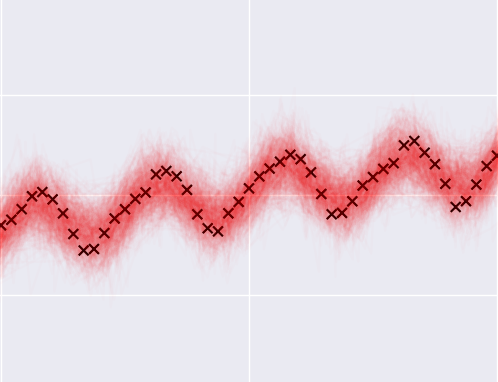
\includegraphics[width=0.2\textwidth]{figs/mauna_zoom.png}};
\node[draw,rectangle,color=red,dashed,left = 3.8cm of zoom, minimum width =
1.5cm, minimum height = 1.2cm,yshift=0.0cm] (zoom_in) {};
\node[below = 1.2cm of post_param_helper_2] (posterior) {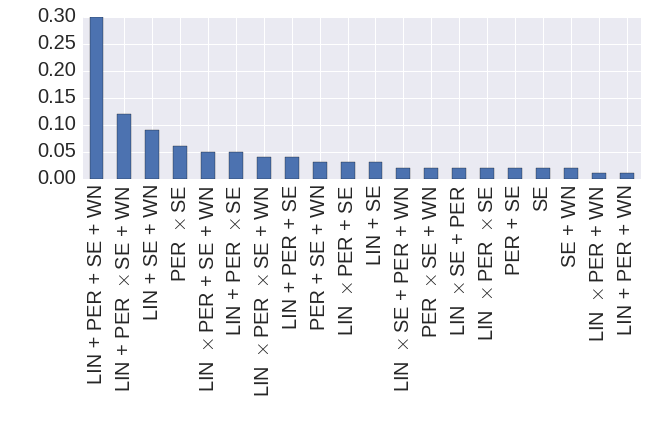
\includegraphics[width=0.6\textwidth]{figs/mauna_structure.png}};

\node[draw,rectangle,below = 1.2cm of posterior] (formula_param_1) {\color{black}\small
$\Ktheta= 2.7^2(x x^\prime) + 5.6^2 \exp \bigg( \frac{2 \sin^2 ( \pi (x - x^\prime)/3.7}{6.4^2} \bigg)
+ 0.4^2 \exp(-\frac{(x-x^\prime)^2}{2 \times 6.3^2}) +  1.9^2 \delta_{x,x^\prime} \label{eq:WN}$ };


\node[draw,rectangle,below = 1.2cm of formula_param_1,text width =
0.9\textwidth,minimum height = 1.5cm,font=\footnotesize] (paragraph){
The posterior peaks at a kernel structure with four additive components. Additive components hold globally, that is there are no higher level, qualitative aspects of the data that vary with the input space. The additive components are as follows: (i) a linearly increasing function or trend; (ii) a periodic function; (iii) a smooth function; and (iv) white noise.};







\node[draw, rectangle, left = -1.75cm of posterior,minimum width = 0.45cm, minimum height = 5.8cm,yshift=0.2cm] (mark_structure) {};
%\node[draw,very thick, rectangle, below = 1.1cm of data,minimum width = \textwidth, minimum height = 15cm] (posterior_frame) {};

%\node[left = 1.3cm of mark_structure] (paragraph_helper){};
\node[below =0.45cm of mark_structure,inner sep = 0pt,outer sep=0pt] (formula_helper) {};
\node[above =1.2cm of formula_param_1,inner sep = 0pt,outer sep=0pt] (formula_helper_2) {};

%\draw[-,dashed] (mark_structure.south) -- (formula_helper);
%\draw[-,dashed] (formula_helper) -- (formula_helper_2);
%\draw[->,dashed] (mark_structure) -- (paragraph_helper);
%\draw[->,dashed] (formula_helper_2) -- (formula);

\draw[->] (data) -- node[right]{\small $\hat \fbf \sim
\mathcal{N}(\hat{\bm{\mu}},\hat\Kbf)$} (post_param_helper_1);
\draw[->] (post_param_helper_2) -- node[right]{\small Posterior Structure} (posterior);
\draw[->] (formula_helper_2) -- node[right] {\small
$\bm{\theta}=\{2.7,5.6,3.7,6.4,0.4,6.3,1.9\}$} (formula_param_1);
\draw[-] (mark_structure) -- node[left, yshift=-0.3cm] {\small $\Ktheta$} (formula_helper);
\draw[-] (formula_helper) --(formula_helper_2);
\draw[->] (formula_param_1) -- node[right]{\small Qualitative Interpretation} (paragraph);

\draw[->,dashed,red] (zoom_in) --node[above]{\small\color{red}Zoom in:}
node[below]{\small\color{red}adequate error bars}(zoom);

%\draw[->,line width=1pt,double distance=2pt] (data) -- (post_param);
% starting from the bottom to aligm with caption 
\node[left=0.3cm of paragraph] (e){(e)}; 

\node[above=1.9cm of e] (d) {(d)}; 
\node[above=5.0cm of d] (c) {(c)}; 
\node[above=4.7cm of c] (b) {(b)}; 
\node[above=4.0cm of b] (a) {(a)}; 
\end{tikzpicture}
\addtolength\abovedisplayskip{1\baselineskip}%
\addtolength\belowdisplayskip{1\baselineskip}%



\caption{\small Posterior of structure and qualitative, human interpretable reading. We take the raw data (top), compute a posterior distribution on structures (red samples and bar plot).
We take the peak of this distribution ($\text{LIN}+\text{PER}+\text{SE}+\text{WN}$) with the sampled parameters used to generate the samples for the second plot from the top and write it in functional form with parameters. We depict the human readable interpretation of the equation on the bottom.}\label{fig:posterior}
\end{figure}

\begin{figure}
\centering
 \addtolength\abovedisplayskip{-1\baselineskip}%
  \addtolength\belowdisplayskip{-1\baselineskip}%
  
\begin{tikzpicture}
\node (datatitle) {\small Raw Data};
\node[below = -0.25cm of datatitle](data) {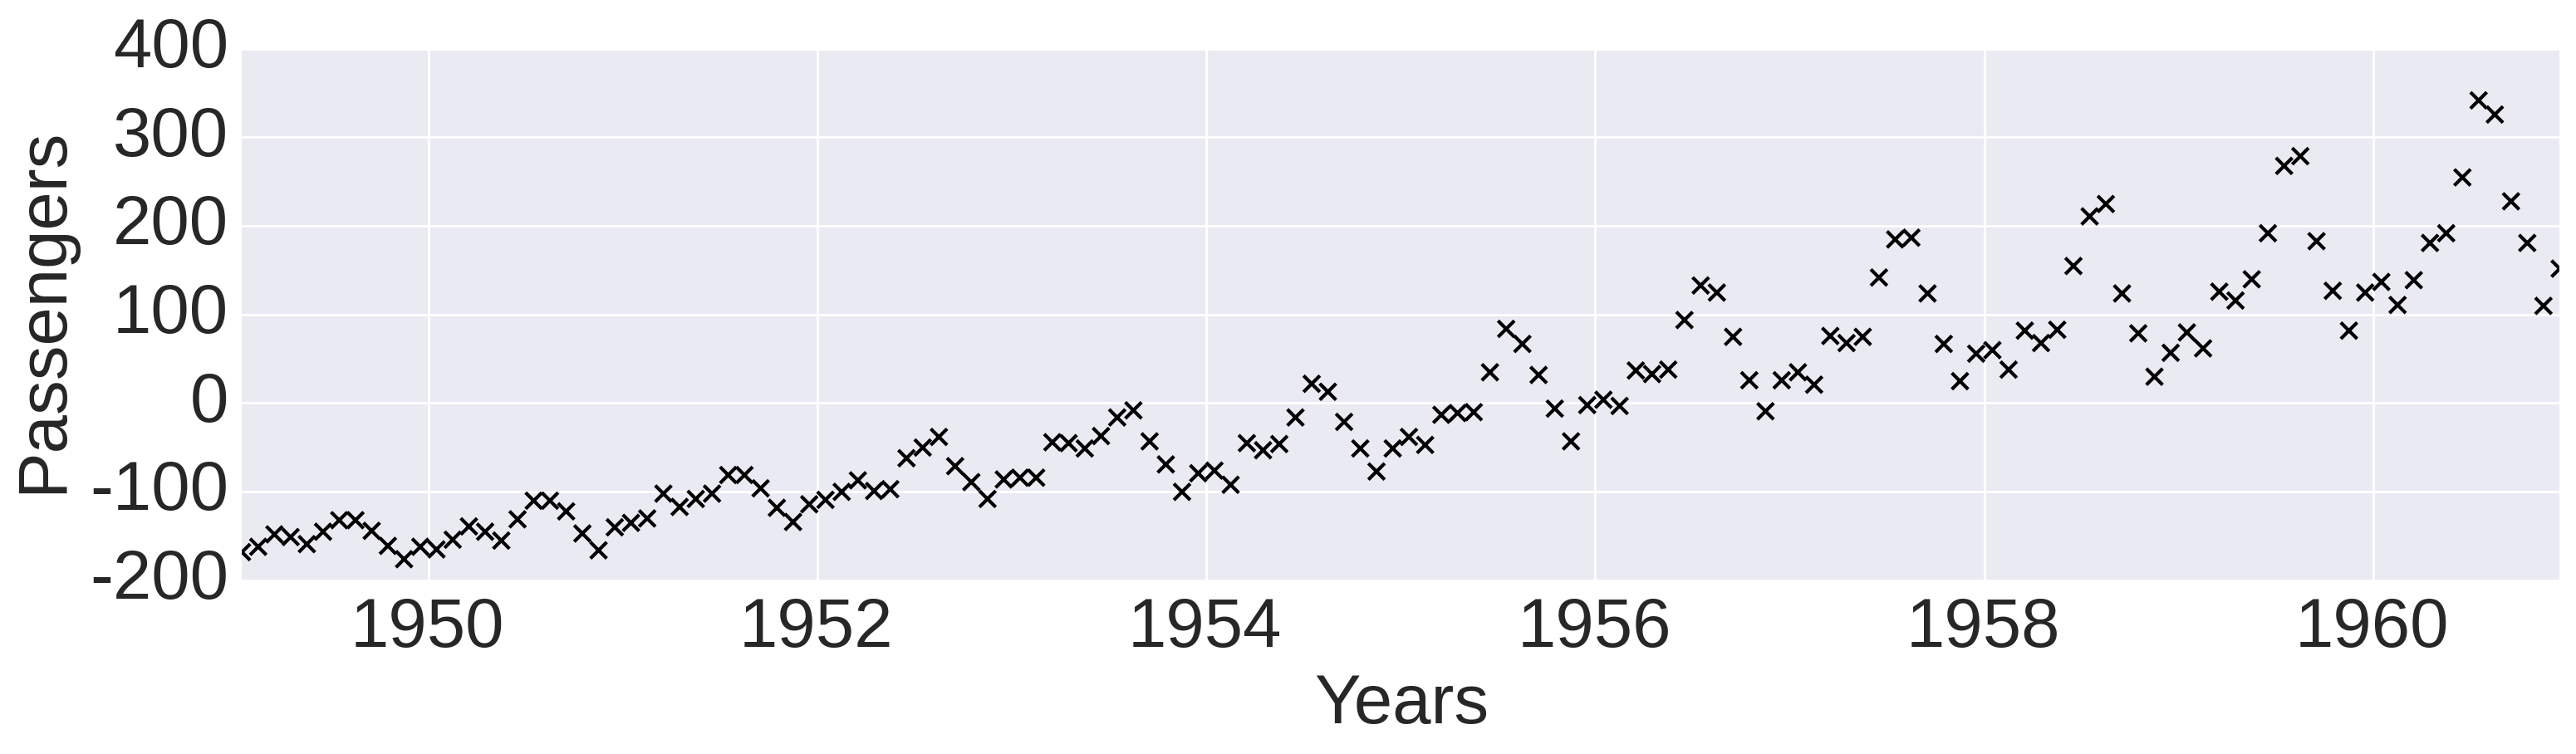
\includegraphics[width=0.65\textwidth]{figs/airline_data.png}};
\node[below= 1.2cm of data] (post_param) {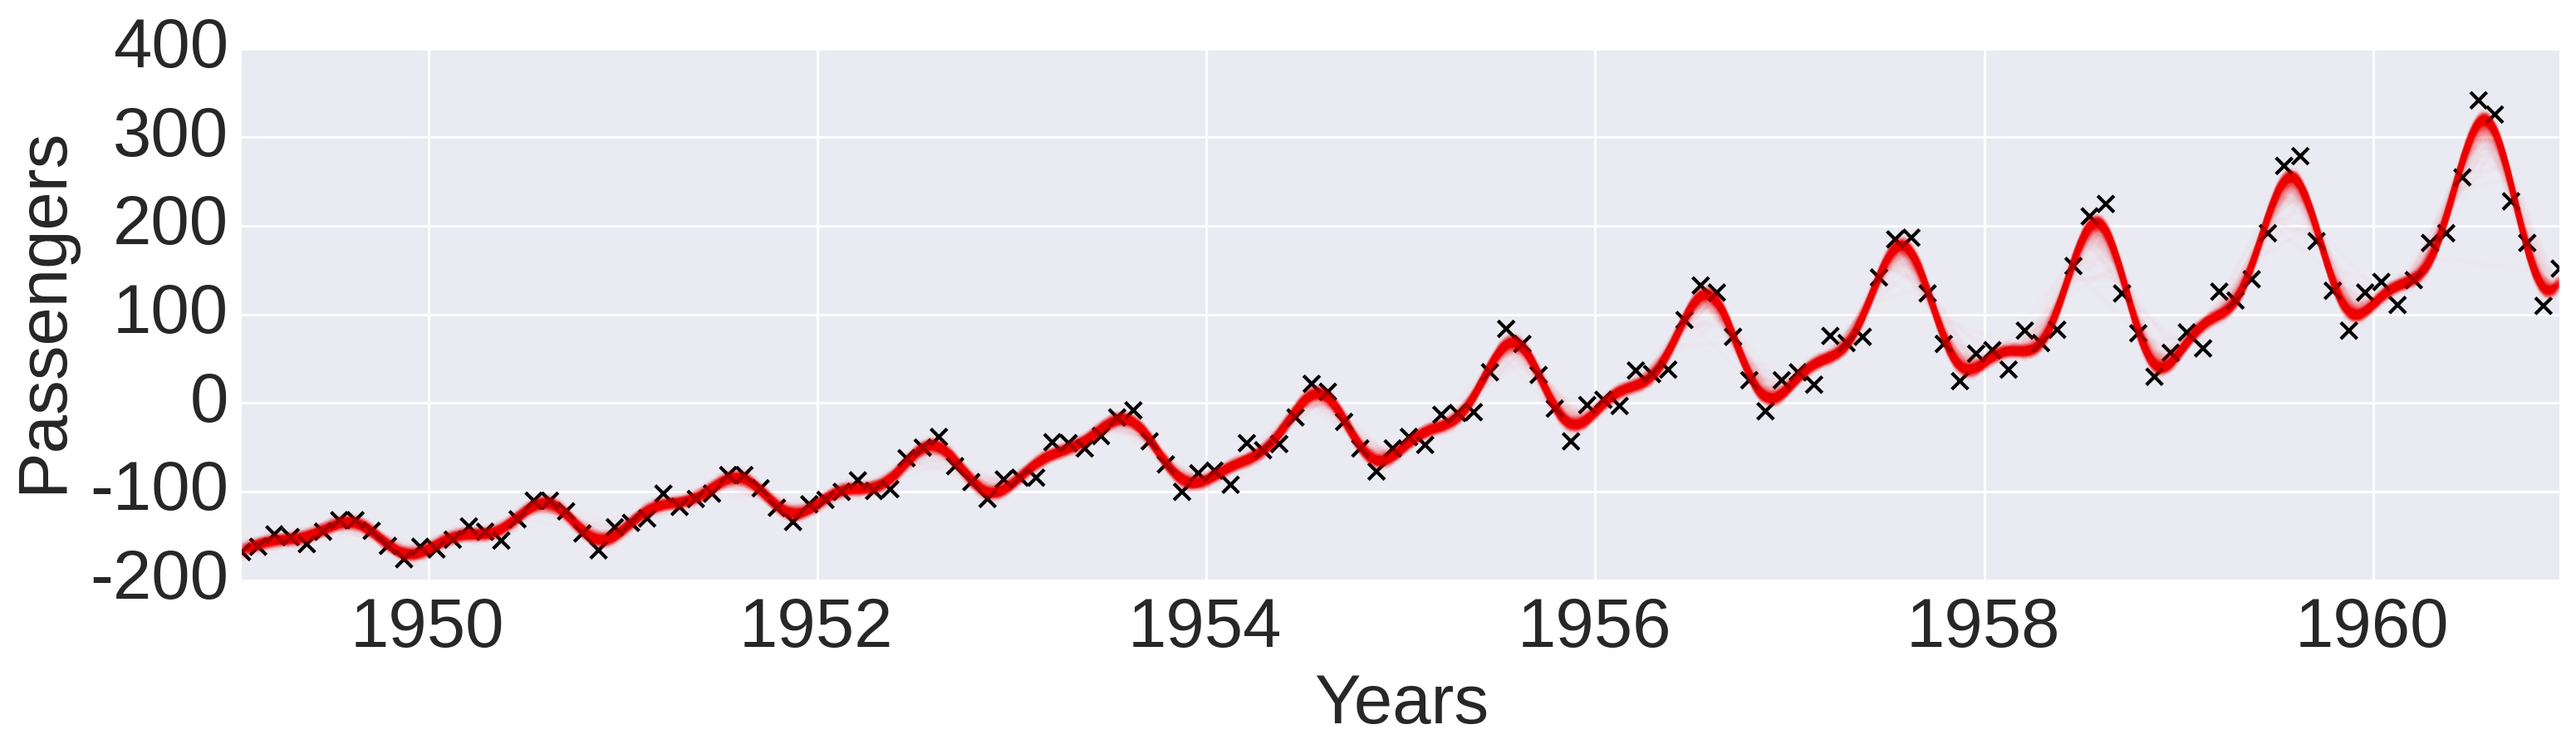
\includegraphics[width=0.65\textwidth]{figs/airline_sample_28.png}};


\node[below = 1.2cm of post_param] (posterior) {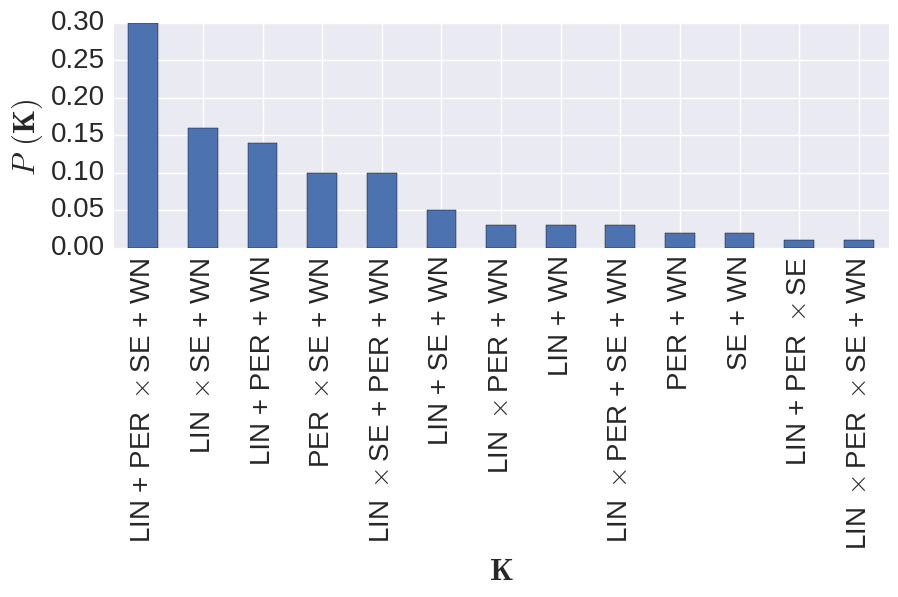
\includegraphics[width=0.55\textwidth]{figs/airline_structure.png}};
\node[below=-0.7cm of posterior,xshift=0.3cm] (xlabel) {\footnotesize
$\Ksrv$};
\node[left =-0.5cm of posterior,yshift=1.3cm] (ylabel) {\rotatebox{90}{\footnotesize
$P(\Ksrv \mid \xbf,\ybf, \thetabf )$}};
\node[draw,rectangle,below = 1.2cm of posterior] (formula_param_1) {\small\color{black}
$\ktheta= 7.47^2(x x^\prime) +
\Bigg(0.27^2 \exp(-\frac{(x-x^\prime)^2}{2 \times 4.63^2}) \times 
7.34^2 \exp \bigg( \frac{2 \sin^2 ( \pi (x - x^\prime)/4.4}{4.55^2} \bigg)\Bigg)
+ 2.93^2 \delta_{x,x^\prime} \label{eq:WN}$ };


\node[draw,rectangle,below = 1.2cm of formula_param_1,text width =0.9\textwidth,minimum height = 1.5cm, font=\footnotesize] (paragraph){ 
The posterior peaks at a kernel structure with three additive components.
Additive components hold globally, that is there are no higher level,
qualitative aspects of the data that vary with the input space. The additive
components are as follows: (i) a linearly increasing function or trend; (ii) an approximate periodic function; and (iv) white noise.};







\node[draw, rectangle, left = -1.7cm of posterior,minimum width = 0.45cm, minimum height = 5.2cm,yshift=0.2cm] (mark_structure) {};
%\node[draw,very thick, rectangle, below = 1.1cm of data,minimum width = \textwidth, minimum height = 15cm] (posterior_frame) {};

%\node[left = 1.3cm of mark_structure] (paragraph_helper){};
\node[below =0.45cm of mark_structure,inner sep = 0pt,outer sep=0pt] (formula_helper) {};
\node[above =1.2cm of formula_param_1,inner sep = 0pt,outer sep=0pt] (formula_helper_2) {};

%\draw[-,dashed] (mark_structure.south) -- (formula_helper);
%\draw[-,dashed] (formula_helper) -- (formula_helper_2);
%\draw[->,dashed] (mark_structure) -- (paragraph_helper);
%\draw[->,dashed] (formula_helper_2) -- (formula);

\draw[->] (data) -- node[right]{\small $\yprime \sim
\mathcal{N}(\mupost,\Kpost)$} (post_param_helper_1);
\draw[->] (post_param_helper_2) -- node[left]{\small }node[right]{\small Marginal on
Structure: $P(\Ksrv \mid \xbf,\ybf,\thetabf )$} (posterior);
\draw[->] (formula_helper_2) -- node[right] {\small
$\bm{\theta}=\{7.47,0.27,4.63,7.34,4.4,4.55,2.93\}$} (formula_param_1);
\draw[-] (mark_structure) -- node[left, yshift=-0.3cm] {\small $\ktheta$} (formula_helper);
\draw[-] (formula_helper) --(formula_helper_2);
\draw[->] (formula_param_1) -- node[right]{\small Qualitative Interpretation} (paragraph);


\node[left=0.3cm of paragraph] (e){(e)}; 

\node[above=1.9cm of e] (d) {(d)}; 
\node[above=5.0cm of d] (c) {(c)}; 
\node[above=4.7cm of c] (b) {(b)}; 
\node[above=4.0cm of b] (a) {(a)}; 
\end{tikzpicture}
\addtolength\abovedisplayskip{1\baselineskip}%
\addtolength\belowdisplayskip{1\baselineskip}%



\caption{\small Posterior of structure and qualitative, human interpretable reading. We take the raw data (top), compute a posterior distribution on structures (red samples and bar plot).
We take the peak of this distribution ($\text{LIN}+\text{PER} \times \text{SE}+\text{WN}$) with the sampled parameters used to generate the samples for the second plot from the top and write it in functional form with parameters. We depict the human readable interpretation of the equation on the bottom.}\label{fig:posterior_airline}
\end{figure}

\begin{figure}
\centering

% 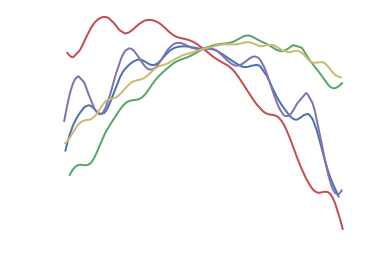
\includegraphics[width=.153\textwidth]{figs/gpSamples/main.png}
\begin{tikzpicture}


% level 1
\node (hyp) {\normalsize \color{blue} What is the probability of a trend, a recurring pattern {\bf and} noise in the data?};
\node[below = -0.2cm of hyp] (hyp_form) {$P\big((\text{LIN}\lor\text{LIN}\times\text{SE})\land
(\text{PER}\lor\text{PER}\times\text{SE}\lor\text{PER}\times\text{LIN})\land
(\text{WN}\lor\text{LIN}\times\text{WN})\big) = 0.36$};

%level 3
\node[below =.5cm of hyp_form , xshift=-3cm] (trend) {\color{blue} Is there a trend?};
\node[below = -0.2cm of trend] (trend_form) {$P(\text{LIN}\lor\text{LIN}\times\text{SE}) = 0.65$};
\node[below = -0.2cm of trend_form] (trend_png) {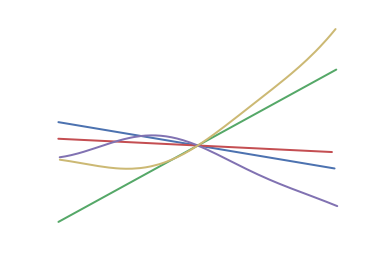
\includegraphics[width=.15\textwidth]{figs/gpSamples/trend.png}};

\node[below =.5cm of hyp_form, xshift=3cm] (noise) {\color{blue} Is there noise? };
\node[below = -0.2cm of noise] (noise_form) {$P(\text{WN}\lor\text{LIN}\times\text{WN}) = 0.75$};
\node[below = -0.2cm of noise_form] (noise_png) {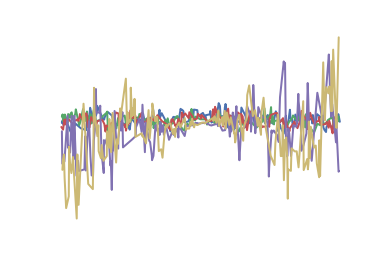
\includegraphics[width=.15\textwidth]{figs/gpSamples/noise.png}};

% level 4
\node[below =.5cm of trend_png , xshift=-2cm] (linear_trend) {\color{blue} A linear trend?};
\node[below = -0.2cm of linear_trend] (linear_trend_form) {$P(\text{LIN}) = 0.63$};
\node[below = -0.2cm of linear_trend_form] (linear_trend_png) {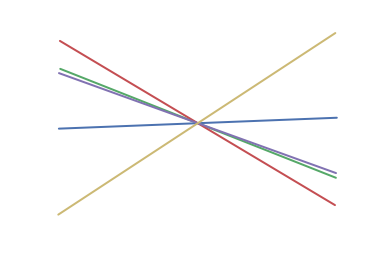
\includegraphics[width=.15\textwidth]{figs/gpSamples/lin.png}};

\node[below =.5cm of trend_png , xshift=1cm] (smooth_trend) {\color{blue} A smooth trend?};
\node[below = -0.2cm of smooth_trend] (smooth_trend_form) {$P(\text{LIN}\times\text{SE}) = 0.02$};
\node[below = -0.2cm of smooth_trend_form] (smooth_trend_png) {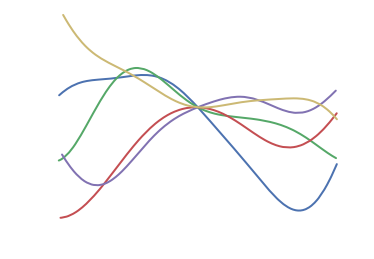
\includegraphics[width=.15\textwidth]{figs/gpSamples/selin.png}};

\node[below =.5cm of noise_png, xshift=-1cm] (het_noise) {\color{blue} Heteroskedastic noise? };
\node[below = -0.2cm of het_noise] (het_noise_form) {$P(\text{LIN}\times\text{WN}) = 0$};
\node[below = -0.2cm of het_noise_form] (het_noise_png) {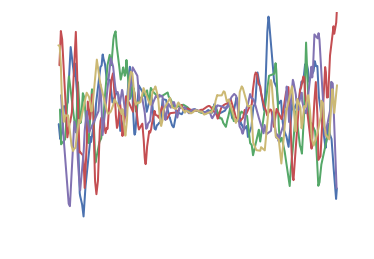
\includegraphics[width=.15\textwidth]{figs/gpSamples/linwn.png}};

\node[below =.5cm of noise_png, xshift=2cm] (white_noise) {\color{blue} White  noise? };
\node[below = -0.2cm of white_noise] (white_noise_form) {$P(\text{WN}) = 0.75$};
\node[below = -0.2cm of white_noise_form] (white_noise_png) {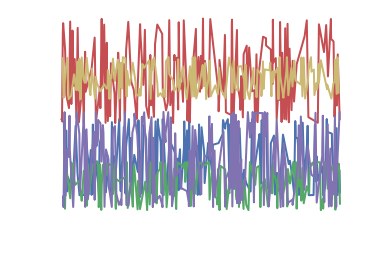
\includegraphics[width=.15\textwidth]{figs/gpSamples/wn.png}};

% level 5
\node[below =6.2cm of hyp_form] (recurring) {\color{blue} Is there repeating structure?};
\node[below = -0.2cm of recurring] (recurring_form) {$P(\text{PER}\lor\text{PER}\times\text{SE}\lor\text{PER}\times\text{LIN}) = 0.73$};
\node[below = -0.2cm of recurring_form] (recurring_png) {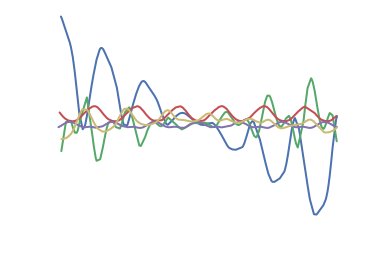
\includegraphics[width=.15\textwidth]{figs/gpSamples/recurring.png}};
%\draw[->,dashed] (barplot) -- (mcmc);

% level 6
\node[below =.5cm of recurring_png] (seper_form) {$\text{PER}\times\text{SE}=0.34$};
\node[below = -0.2cm of seper_form] (seper_png) {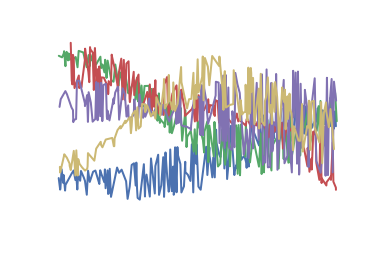
\includegraphics[width=.15\textwidth]{figs/gpSamples/seper.png}};

\node[below =.5cm of recurring_png, xshift=-3cm] (per_form) {$\text{PER}=0.32$};
\node[below = -0.2cm of per_form] (per_png) {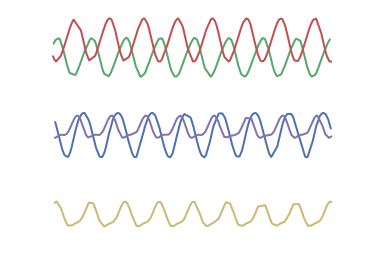
\includegraphics[width=.15\textwidth]{figs/gpSamples/per.png}};

\node[below =.5cm of recurring_png,xshift=3cm] (perlin_form) {$\text{PER}\times\text{LIN}=0.07$};
\node[below = -0.2cm of perlin_form] (seper_png) {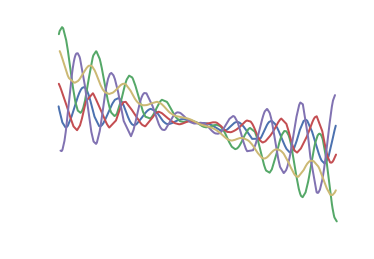
\includegraphics[width=.15\textwidth]{figs/gpSamples/perlin.png}};





\draw[->] (hyp_form) -- (trend);
\draw[->] (hyp_form) -- (noise);
\draw[->] (hyp_form) -- (recurring);


\draw[->] (noise_png) -- (het_noise);
\draw[->] (noise_png) -- (white_noise);

\draw[->] (trend_png) -- (linear_trend);
\draw[->] (trend_png) -- (smooth_trend);

\draw[->] (recurring_png) -- (per_form);
\draw[->] (recurring_png) -- (seper_form);
\draw[->] (recurring_png) -- (perlin_form);


\end{tikzpicture}



%  \multicolumn{3}{c}{$P(\text{PER}\lor\text{PER}\times\text{SE}\lor\text{PER}\times\text{LIN})$}

\caption{We can query the data if some logical statements are probable to be true, for example, is it true that there is a trend?}\label{fig:query}
\end{figure}

\subsection{Bayesian optimization}

\label{sec:thompson}



The final application demonstrating the power of \gpmem\ demonstates its use in Bayesian optimization. We introduce Thompson sampling, the basic solution strategy
underlying the Bayesian optimization with \gpmem.
Thompson sampling~\cite{thompson1933likelihood} is a widely used Bayesian
framework for addressing the trade-off between exploration and exploitation in
multi-armed (or continuum-armed) bandit problems.  
We cast the multi-armed bandit problem as a one-state Markov
decision process (MDP), and describe how Thompson sampling can be used to choose
actions for that MDP.

The MDP is as follows: An agent is to take a sequence of actions $a_1, a_2,
\ldots$ from a (possibly infinite) set of possible actions $\Acal$.  After each
action, a reward $r \in \R$ is received, according to an unknown conditional
distribution $P_\true\pn{r \mvert a}$.  The agent's goal is to maximize the
total reward received for all actions in an online manner.  In Thompson
sampling, the agent accomplishes this by placing a prior distribution
$P(\ttheta)$ on the possible ``contexts'' $\ttheta \in \Theta$.  Here a context
is a believed model of the conditional distributions $\{P\pn{r \mvert a}\}_{a
\in \Acal}$, or at least, a believed statistic of these conditional
distributions which is sufficient for deciding an action $a$.  If actions are
chosen so as to maximize expected reward, then one such sufficient statistic is
the believed conditional mean $V\pn{a \mvert \ttheta} = \Ebkt{r \mvert
a;\ttheta}$, which can be viewed as a believed value function.  For
consistency with what follows, we will assume our context $\ttheta$ takes the
form $(\theta, \abf_\past, \rbf_\past)$ where $\abf_\past$ is the vector of past
actions, $\rbf_\past$ is the vector of their rewards, and $\theta$ (the
``semicontext'') contains any other information that is included in the context.

In this setup, Thompson sampling has the following steps:
\begin{algorithm}[H]
  \singlespacing
  Repeat as long as desired:
  \begin{enumerate}
    \item\label{itm:thompson-step-sample} {\bf Sample.} Sample a semicontext
      $\theta \sim P(\theta)$.
    \item\label{itm:thompson-step-search} {\bf Search (and act).} Choose an
      action $a \in \Acal$ which (approximately) maximizes $V\pn{a \mvert
      \ttheta} = \Ebkt{r \mvert a; \ttheta} = \Ebkt{r \mvert a;\,\theta,
      \abf_\past, \rbf_\past}$.
    \item {\bf Update.} Let $r_\true$ be the reward received for action $a$.
      Update the believed distribution on $\theta$, i.e., $P(\theta) \gets
      P_\rmnew(\theta)$ where $P_\rmnew(\theta) = P\pn{\theta \mvert a \mapsto
      r_\true}$.
  \end{enumerate}
  \caption{Thompson sampling.}
  \label{alg:thompson}
\end{algorithm}
Note that when $\Ebkt{r|a;\ttheta}$ (under the sampled value of $\theta$ for
some points $a$) is far from the true value $\Ebkt[P_\true]{r \mvert a}$, the
chosen action $a$ may be far from optimal, but the information gained by probing
action $a$ will improve the belief $\ttheta$.  This amounts to ``exploration.''
When $\Ebkt{r \mvert a;\ttheta}$ is close to the true value except at points $a$
for which $\Ebkt{r \mvert a;\ttheta}$ is low, exploration will be less likely to
occur, but the chosen actions $a$ will tend to receive high rewards.  This
amounts to ``exploitation.'' The trade-off between exploration and exploitation
is illustrated in Figure \ref{fig:slide2}.  Roughly speaking, exploration will
happen until the context $\ttheta$ is reasonably sure that the unexplored
actions are probably not optimal, at which time the Thompson sampler will
exploit by choosing actions in regions it knows to have high value.

\begin{figure}
  \centering
  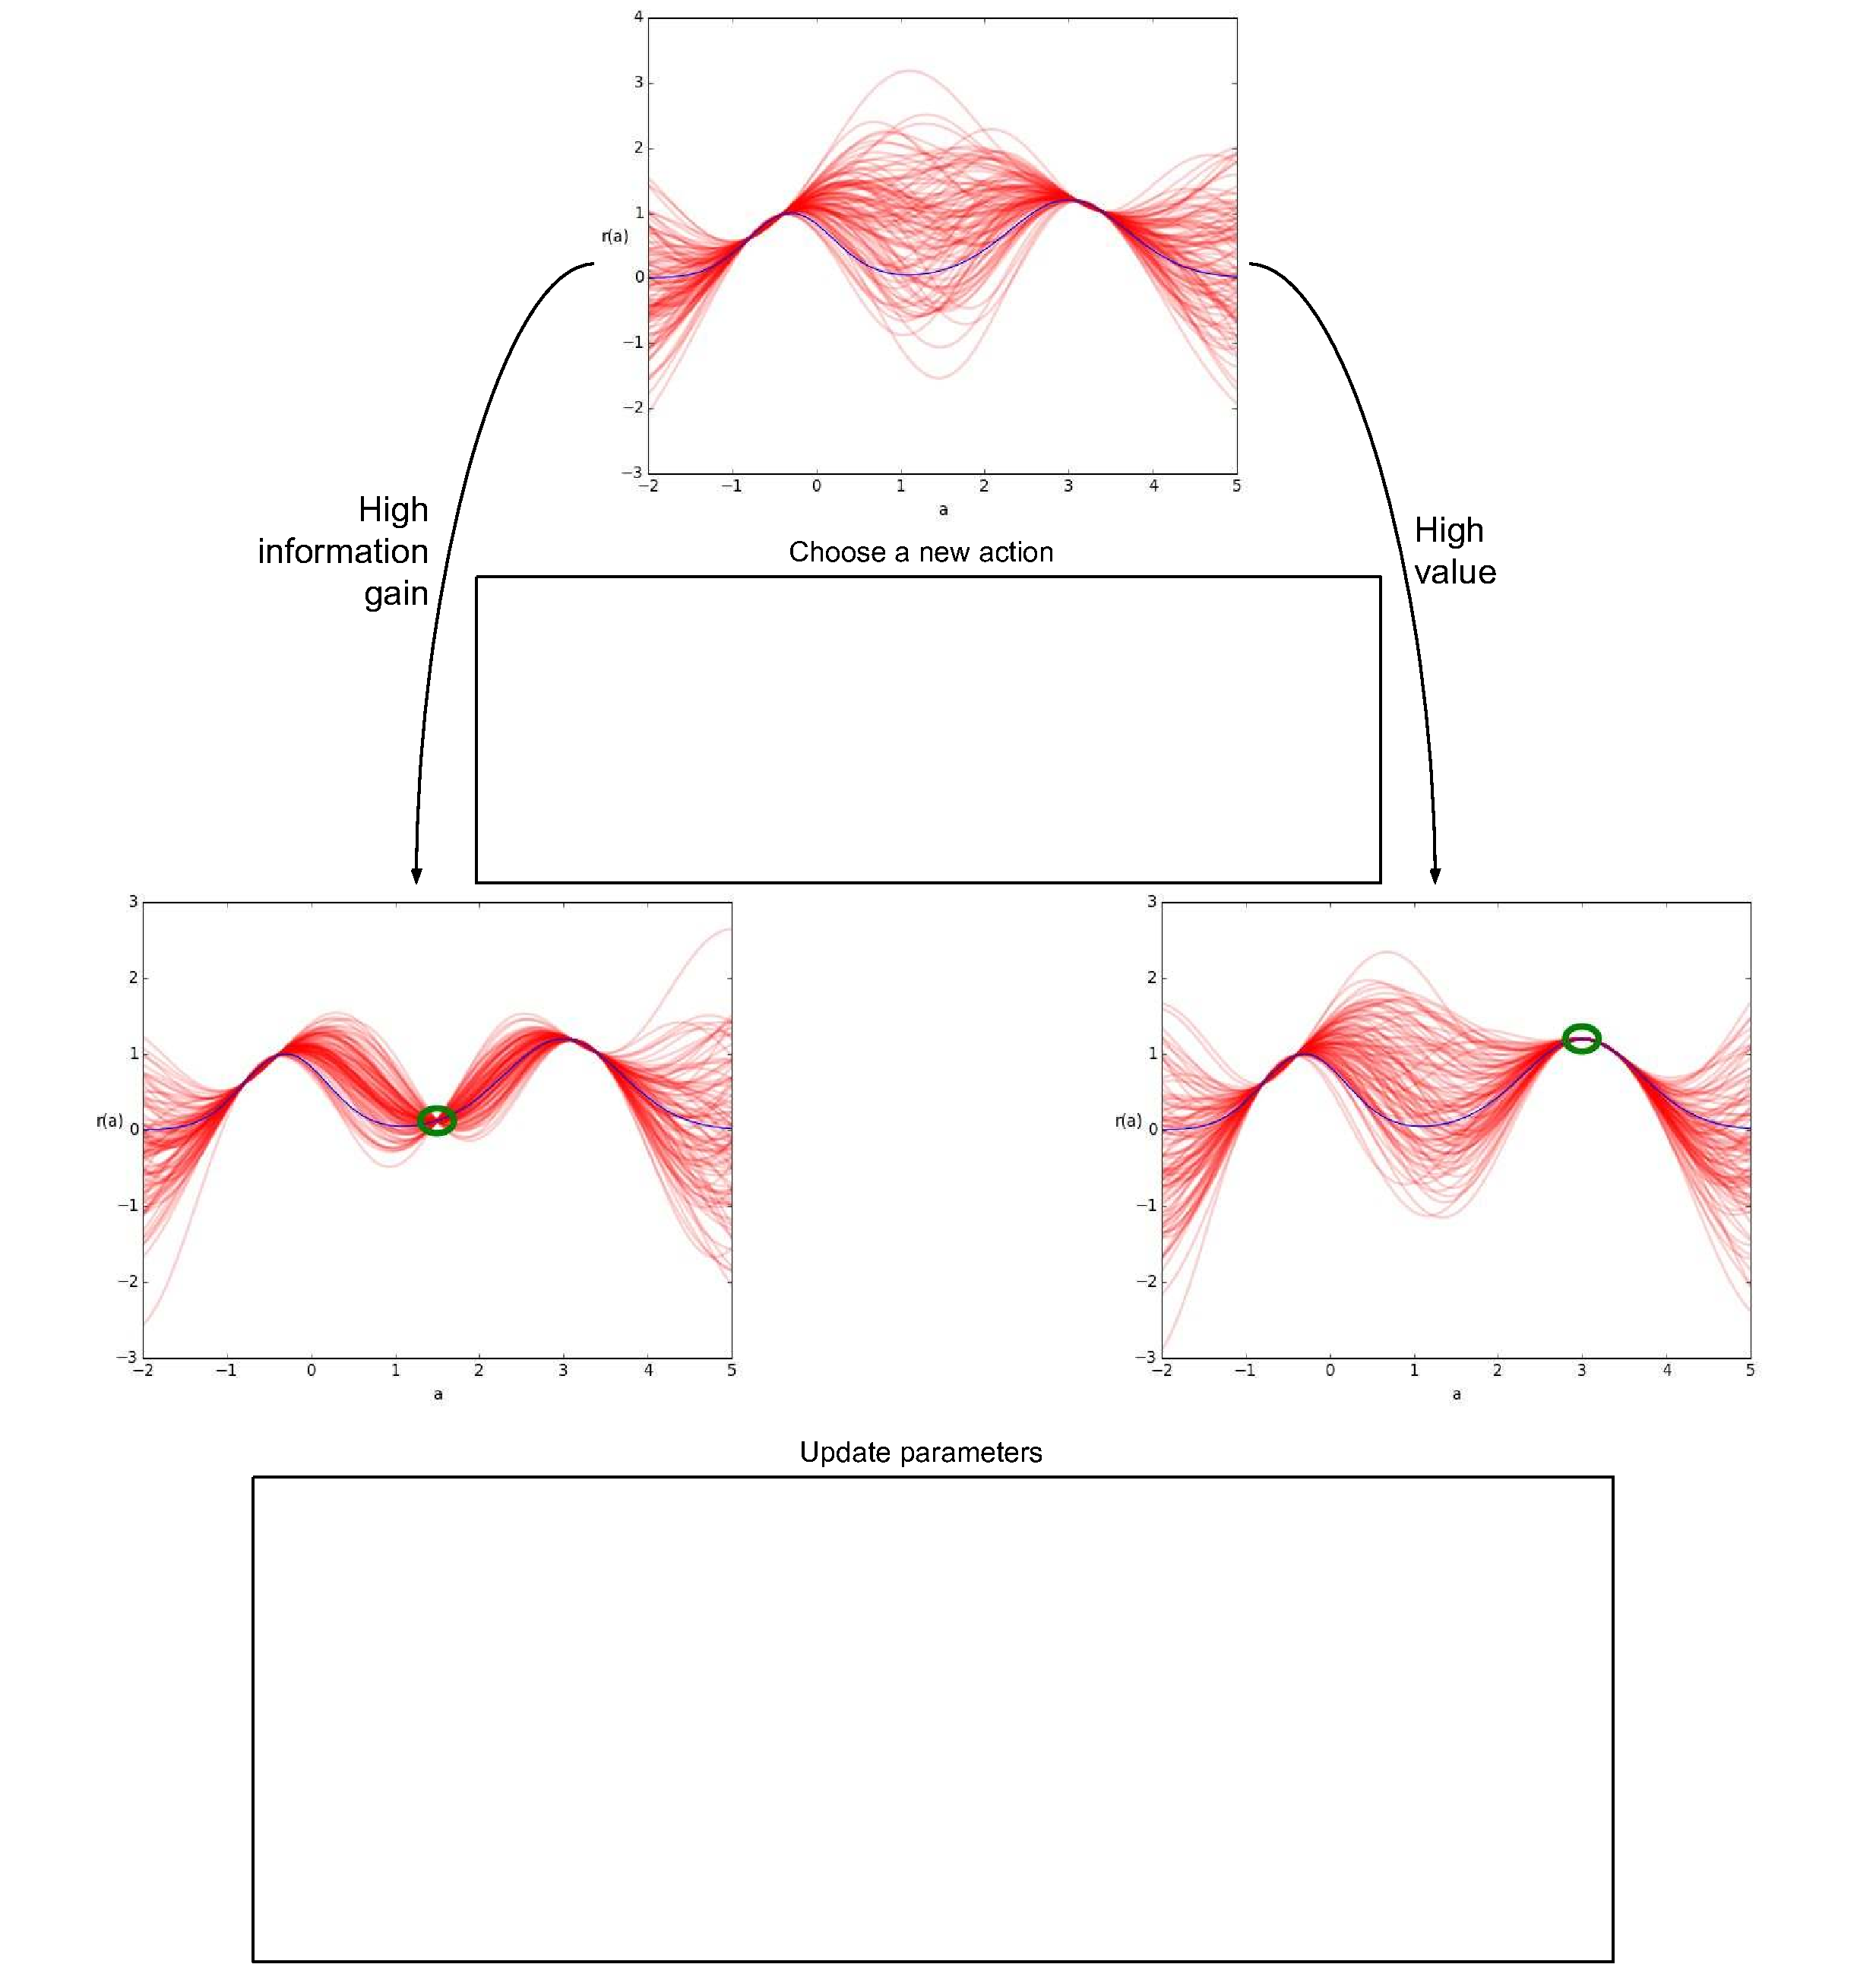
\includegraphics[width=\linewidth]{figs/slide2.pdf}
  \caption{
    Two possible actions (in green) for an iteration of Thompson sampling.  The
    believed distribution on the value function $V$ is depicted in red.  In this
    example, the true reward function is deterministic, and is drawn in blue.
    The action on the right receives a high reward, while the action on the left
    receives a low reward but greatly improves the accuracy of the believed
    distribution on $V$.  The transition operators $\tau_\search$ and
    $\tau_\update$ are described in Section \ref{sec:math-spec}.
  }
  \label{fig:slide2}
\end{figure}

Typically, when Thompson sampling is implemented, the search over contexts
$\ttheta \in \Theta$ is limited by the choice of representation.  In
traditional programming environments, $\theta$ often consists of a few
numerical parameters for a family of distributions of a fixed functional
form.  With work, a mixture of a few functional forms is possible; but
without probabilistic programming machinery, implementing a rich context
space $\Theta$ would be an unworkably large technical burden.  In a
probabilstic programing language, however, the representation of
heterogeneously structured or infinite-dimensional context spaces is quite
natural.  Any computable model of the conditional distributions
$\br{P\pn{r \mvert a}}_{a \in \Acal}$ can be represented as a stochastic
procedure $(\lambda (a) \ldots)$.  Thus, for computational Thompson sampling,
the most general context space $\widehat\Theta$ is the space of program texts.
Any other context space $\Theta$ has a natural embedding as a subset of
$\widehat\Theta$.
\begin{comment}
\myparagraph{Thompson Sampling with a Statistical Memoizer}
\label{sec:thompson-mem-em}
Thompson sampling as described above can be expressed compactly in terms of a
statistical memoizer, as in Listing \ref{lst:thompson-mem-em} (see also Figure
\ref{fig:slide1}).  Here and in what follows, to simplify the treatment, we
assume the true reward function is deterministic, i.e., for each fixed $a$, the
conditional distribution $P_\true\pn{r \mvert a}$ is a delta distribution.  We
thus treat the notations $a,r,\abf_\past,\rbf_\past$ as synonyms for
$x,y,\xbf_\past,\ybf_\past$, respectively, differing only in that they carry the
connotations of ``action'' and ``reward.''

\begin{mdframed}
\begin{minipage}{\linewidth}
\small
\belowcaptionskip=-10pt
\begin{lstlisting}[escapechar=\#,language=Venture,label=lst:thompson-mem-em,caption={
  Code template for Thompson sampling in pseudo-Venture using a statistical
  memoizer.  The choice of statistical memoizer (\texttt{mem\&em}), prior on
  semicontexts (\texttt{prior\_on\_semicontexts}), and approximation strategy
  for maximizing the emulator (\texttt{argmax}) are not included.
}]
#\linenumber{1}#assume theta = tag(quote( theta ), 0,  prior_on_semicontexts())
#\linenumber{2}#assume (r_probe r_emulate) = mem&em( do_action, theta)

#\linenumber{3}#infer repeat(15, do(pass,
#\linenumber{4}#     a = mc_argmax(r_emulate, quote(_)),
#\linenumber{5}#     r_probe(a)
#\linenumber{6}#     mh(quote(theta), one, 50)))
\end{lstlisting}
\end{minipage}
\end{mdframed}

\FloatBarrier

In Listing \ref{lst:thompson-mem-em}, \texttt{do\_action} is a procedure which
interfaces with the outside environment and returns the reward received.
\texttt{do\_action} is wrapped in the statistical memoizer \texttt{mem\&em},
with parameters given by the semicontext \texttt{theta} (see Setion
\ref{sec:thompson-framework}).  \texttt{theta} is given a prior distribution,
and as more actions \texttt{a} are probed, inference is performed on
\texttt{theta}, and subsequent evaluations of the emulator \texttt{r\_emulate}
are affected accordingly.  The action \texttt{a} chosen at each step is
determined by the procedure \texttt{argmax}; for purposes of Thompson sampling,
\texttt{argmax} (which takes a possibly stochastic procedure as its argument)
should be implemented so that \texttt{(argmax func)} returns an approximation to
$\argmax_{\texttt{a}} \Ebkt{\texttt{(func a)}}$.

\begin{figure}[p]
  \centering
  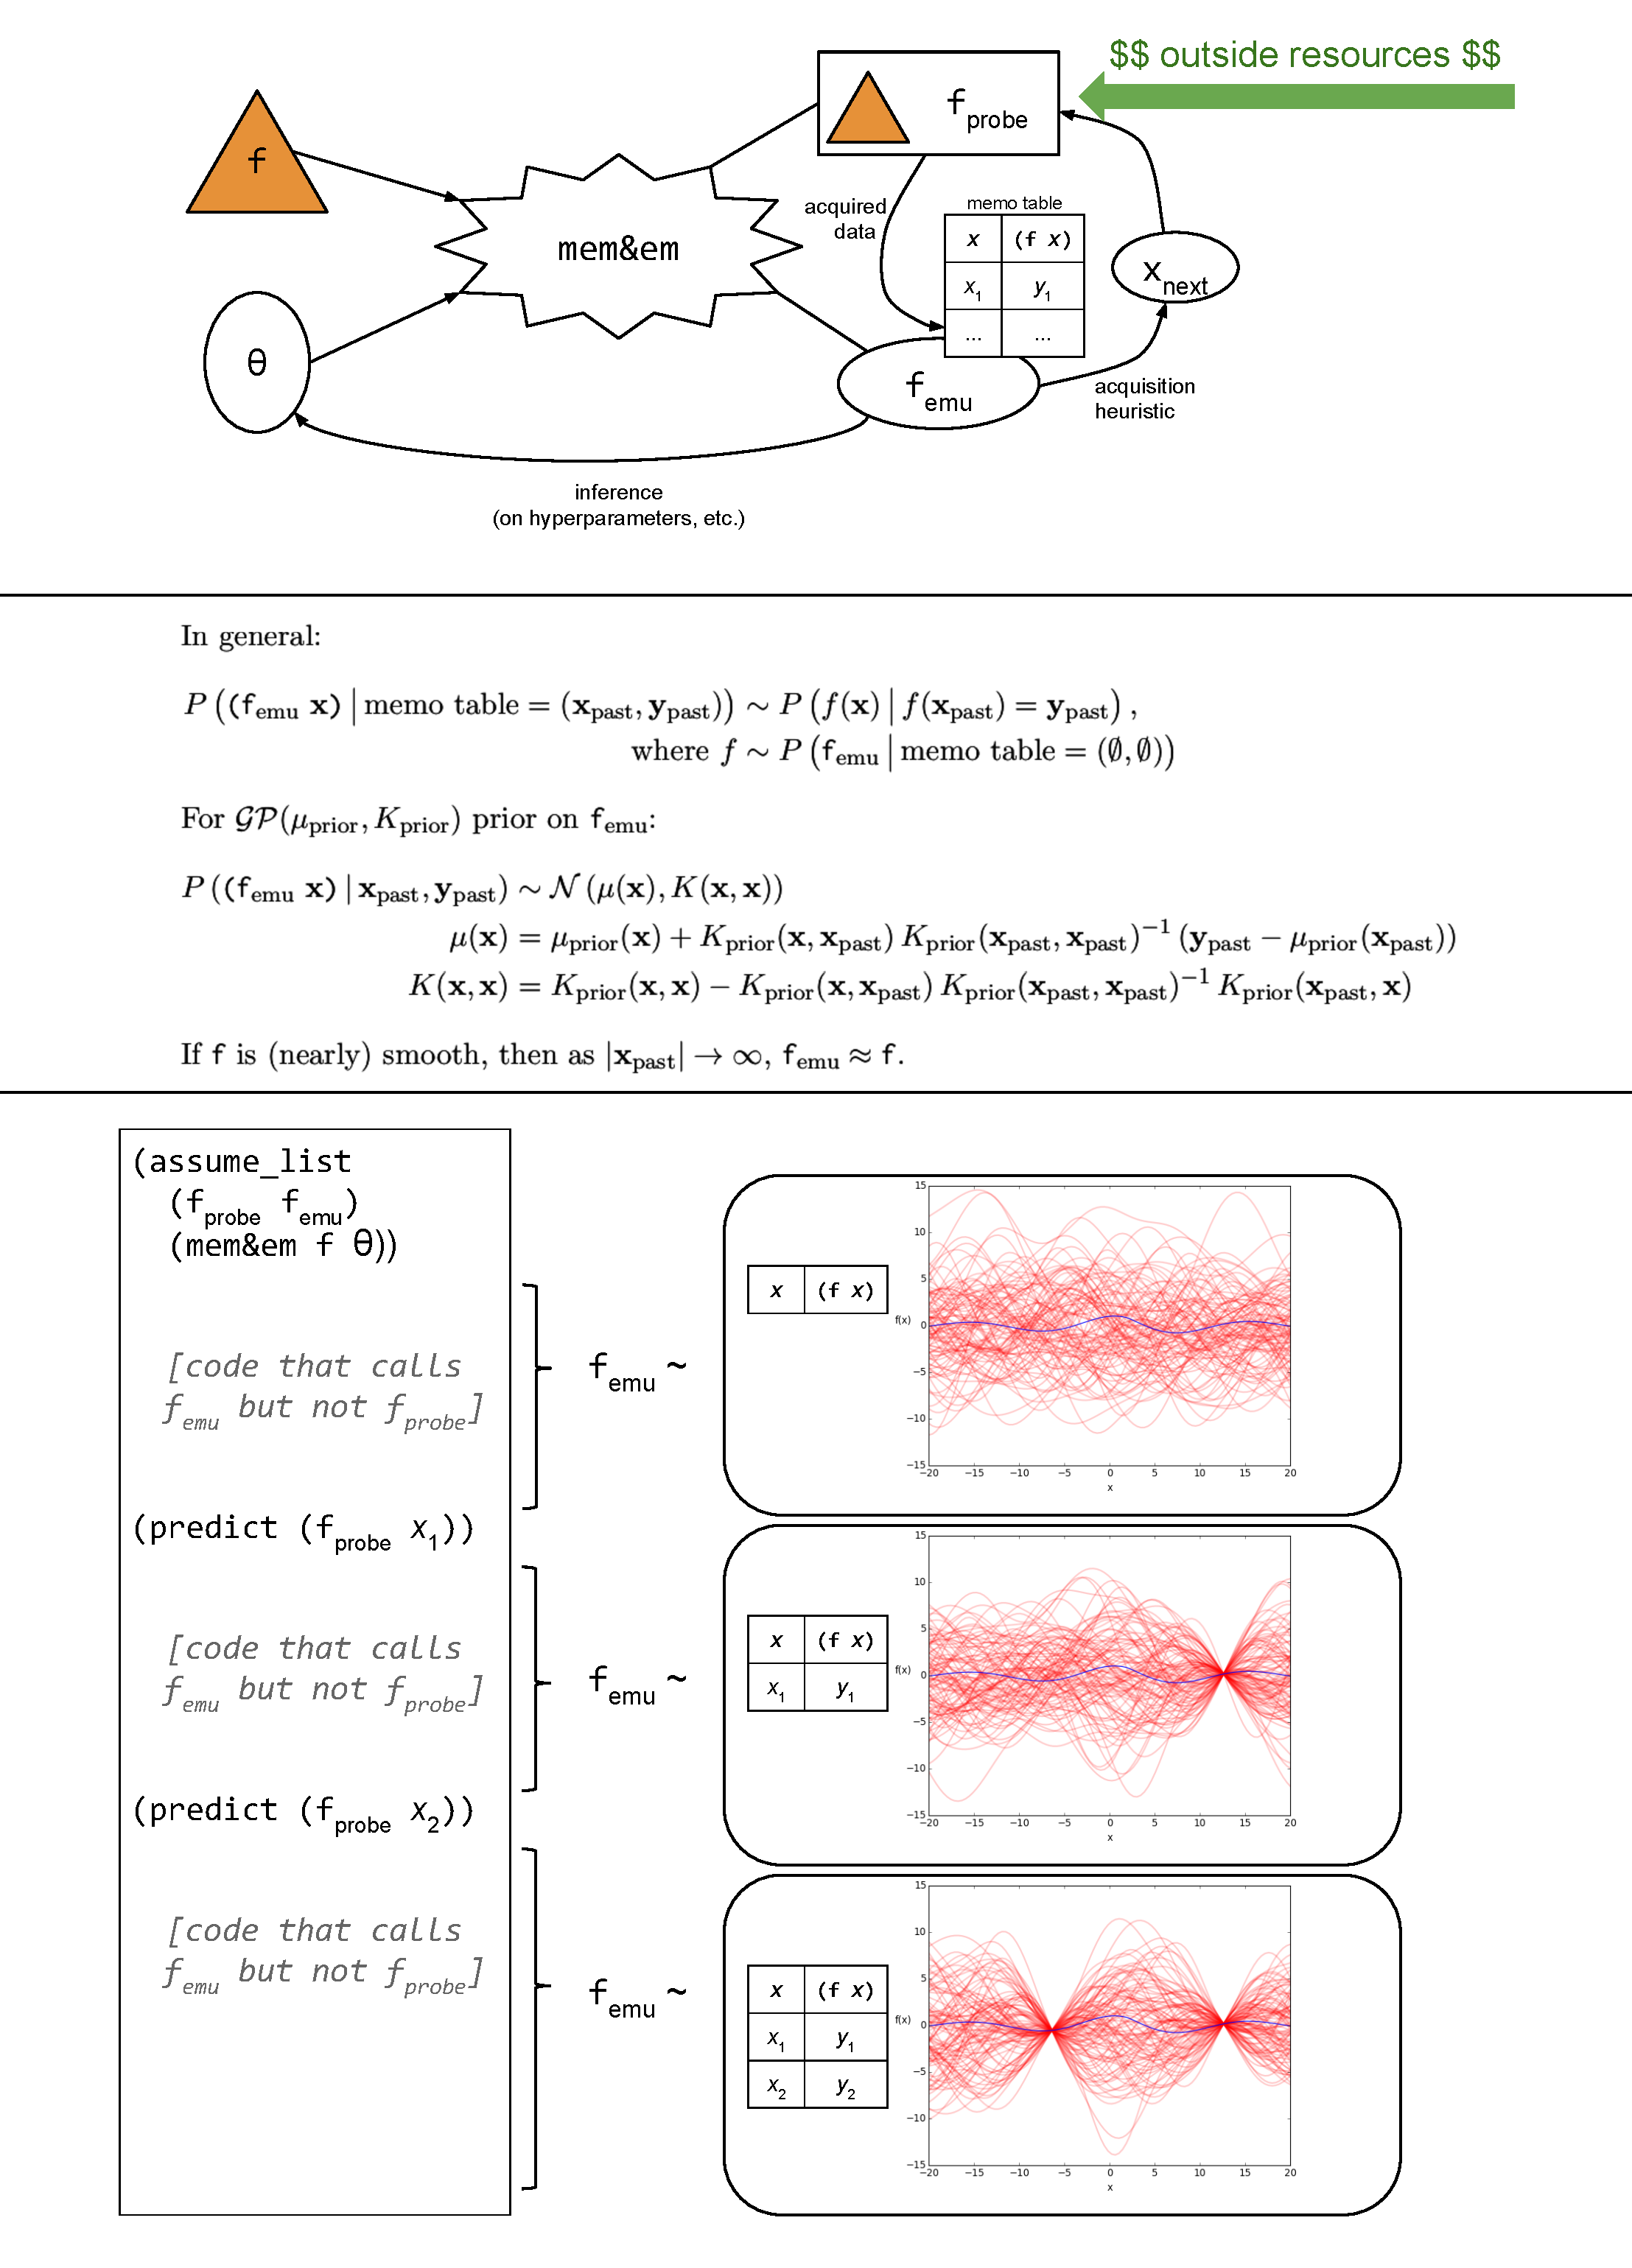
\includegraphics[height=0.8\textheight]{figs/slide1.pdf}
  \caption{
    Top: Diagrammatic representation of Thompson sampling using the statistical
    memoizer $\mm$.  The emulator $\ftt_\emu$ is used to choose a point
    $\xtt_\rmnext$ to acquire; the acquired data are incorporated into the memo
    table and the parameters $\theta$ are updated according to this new
    information.
    Middle: Mathematical specification of the statistical emulator $\ftt_\emu$.
    Bottom: Depiction of the state of the emulator after zero, one, and two
    probes have been taken.  Here the true value function $V$ is drawn in blue;
    the believed distribution on $V$ is drawn in red.  Between probes,
    $\ftt_\emu$ can be \texttt{sample}d but not \texttt{predict}ed, as its state
    (see Section \ref{sec:gps-in-pps}) must not be changed.  The state (i.e.,
    the memo table) must only be changed when $\ftt_\probe$ is called.
  }
  \label{fig:slide1}
\end{figure}
\end{comment}
\myparagraph{A Mathematical Specification}\label{sec:math-spec}
We now describe a particular case of Thompson sampling with the following properties:
\begin{itemize}
  \item The regression function has a Gaussian process prior.
  \item The actions $a_1,a_2,\ldots \in \Acal$ are chosen by a Metropolis-like search
    strategy with Gaussian drift proposals.
  \item The hyperparameters of the Gaussian process are inferred using
    Metropolis--Hastings sampling after each action.
\end{itemize}

In this version of Thompson sampling, the contexts $\ttheta$ are Gaussian
processes over the action space $\Acal = [-20, 20] \subseteq \R$.  That is,
\[ V \sim \GP(\mu, K), \]
where the mean $\mu$ is a computable function $\Acal \to \R$ and the covariance
$K$ is a computable (symmetric, positive-semidefinite) function $\Acal \times
\Acal \to \R$.  This represents a Gaussian process $\br{R_a}_{a \in \Acal}$,
where $R_a$ represents the reward for action $a$.  Computationally, we represent
a context as a data structure
\[ \ttheta = (\theta, \abf_\past, \rbf_\past) = (\mu_\prior, K_\prior, \eta, \abf_\past, \rbf_\past), \]
where $\mu_\prior$ is a procedure to be used as the prior mean function and
$K_\prior$ is a procedure to be used as the prior covariance function, parameterized by 
$\eta$.
We set $\mu_\prior \equiv 0$.

The posterior mean and covariance for such a context $\ttheta$ are gotten by the
usual conditioning formulas (assuming, for ease of exposition as above, that the
prior mean is zero):\footnote{
  Here, for vectors $\abf = \pn{a_i}_{i=1}^{n}$ and $\abf' =
  \pn{a'_i}_{i=1}^{n'}$, $\mu(\abf)$ denotes the vector
  $\pn{\mu(a_i)}_{i=1}^{n}$ and $K(\abf,\abf')$ denotes the matrix
  $\begin{bmatrix} K(a_i, a'_j) \end{bmatrix}_{1 \leq i \leq n, 1 \leq j
  \leq n'}$.
}
\begin{align*}
  \mu(\abf)
  &= \mu\pn{\abf \mvert \abf_\past, \rbf_\past} \\
  &= K_\prior(\abf, \abf_\past)
     \,K_\prior(\abf_\past, \abf_\past)^{-1}
     \,\rbf_\past \\
  K(\abf, \abf)
  &= K\pn{\abf, \abf \mvert \abf_\past, \rbf_\past} \\
  &= K_\prior(\abf, \abf)
     - K_\prior(\abf, \abf_\past)
       \,K_\prior(\abf_\past, \abf_\past)^{-1}
       \,K_\prior(\abf_\past, \abf).
\end{align*}
Note that the context space $\Theta$ is not a finite-dimensional parametric
family, since the vectors $\abf_\past$ and $\rbf_\past$ grow as more samples are
taken.  $\Theta$ is, however, representable as a computational
procedure together with parameters and past samples, as we do in the
representation $\ttheta = (\mu_\prior, K_\prior, \eta, \abf_\past, \rbf_\past)$.

We combine the Update and Sample steps of Algorithm \ref{alg:thompson} by
running a Metropolis--Hastings (MH) sampler whose stationary distribution is the
posterior $P\pn{\theta \mvert \abf_\past, \rbf_\past}$.  The functional forms of
$\mu_\prior$ and $K_\prior$ are fixed in our case, so inference is only done
over the parameters $\eta = \br{\sigma,\ell}$; hence we equivalently write
$P\pn{\sigma,\ell \mvert \abf_\past, \rbf_\past}$ for the stationary
distribution.  We make MH proposals to one variable at a time, using the prior
as proposal distribution:
\[
  Q_\proposal\pn{\sigma',\ell \mvert \sigma,\ell} = P(\sigma')
\]
and
\[
  Q_\proposal\pn{\sigma,\ell' \mvert \sigma,\ell} = P(\ell').
\]
The MH acceptance probability for such a proposal is
\[
  P_\accept\pn{\sigma',\ell' \mvert \sigma,\ell}
  =
  \min\br{1,\ \frac{
    Q_\proposal\pn{\sigma,\ell \mvert \sigma',\ell'}
    }{
    Q_\proposal\pn{\sigma',\ell' \mvert \sigma,\ell}
    }
  \cdot
  \frac{
    P\pn{\abf_\past,\rbf_\past \mvert \sigma',\ell'}
    }{
    P\pn{\abf_\past,\rbf_\past \mvert \sigma,\ell}
    }}
\]
Because the priors on $\sigma$ and $\ell$ are uniform in our case, the term
involving $Q_\proposal$ equals $1$ and we have simply
\begin{align*}
  P_\accept\pn{\sigma',\ell' \mvert \sigma,\ell}
  &=
  \min\br{1,\ \frac{
    P\pn{\abf_\past,\rbf_\past \mvert \sigma',\ell'}
    }{
    P\pn{\abf_\past,\rbf_\past \mvert \sigma,\ell}
    }} \\[2mm]
  &=
  \min\bigg\{1,\ \exp\bigg( -\frac12\bigg(
    \rbf_\past^T K_\prior\pn{\abf_\past, \abf_\past \mvert \sigma', \ell'}^{-1} \rbf_\past \\
  & \qquad\qquad\qquad\qquad\qquad -
    \rbf_\past^T K_\prior\pn{\abf_\past, \abf_\past \mvert \sigma, \ell}^{-1} \rbf_\past
  \bigg)\bigg)\bigg\}.
\end{align*}
The proposal and acceptance/rejection process described above define a
transition operator $\tau_\update$ which is iterated a specified number of
times; the resulting state of the MH Markov chain is taken as the sampled
semicontext $\theta$ in Step \ref{itm:thompson-step-sample} of Algorithm
\ref{alg:thompson}.

For Step \ref{itm:thompson-step-search} (Search) of Thompson sampling, we
explore the action space using an MH-like transition operator $\tau_\search$.
As in MH, each iteration of $\tau_\search$ produces a proposal which is either
accepted or rejected, and the state of this Markov chain after a specified
number of steps is the new action $a$.  The Markov chain's initial state is the
most recent action, and the proposal distribution is Gaussian drift:
\[ Q_\proposal\pn{a' \mvert a} \sim \Ncal(a,\,\propstd^2), \]
where the drift width $\propstd$ is specified ahead of time.  The acceptance
probability of such a proposal is
\[ P_\accept\pn{a' \mvert a} = \min\br{1,\ \exp\pn{-E\pn{a' \mvert a}}}, \]
where the energy function $E\pn{\bullet \mvert a}$ is given by a Monte Carlo
estimate of the difference in value from the current action:
\[ E\pn{a' \mvert a} = -\frac1s \pn{\muhat(a') - \muhat(a)} \]
where
\[ \muhat(a) = \frac{1}{N_\avg} \sum_{i=1}^{N_\avg} \widetilde{r}_{i,a} \]
and
\[ \widetilde{r}_{i,a} \sim \Ncal(\mu(a), K(a,a)) \]
and $\br{\widetilde{r}_{i,a}}_{i=1}^{N_\avg}$ are i.i.d.\ for a fixed $a$.
Here the temperature parameter $s \geq 0$ and the population size $N_\avg$ are
specified ahead of time.  Proposals of estimated value higher than that of the current action are
always accepted, while proposals of estimated value lower than that of the
current action are accepted with a probability that decays exponentially
with respect to the difference in value.
The rate of the decay is determined by the temperature parameter $s$,
where high temperature corresponds to generous acceptance probabilities.
For $s=0$, all proposals of lower value are rejected; for $s=\infty$, all
proposals are accepted.
For points $a$ at which the posterior mean $\mu(a)$ is low but the
posterior variance $K(a,a)$ is high, it is possible (especially when
$N_\avg$ is small) to draw a ``wild'' value of $\muhat(a)$, resulting in a
favorable acceptance probability.



Indeed, taking an action $a$ with low estimated value but high uncertainty
serves the useful function of improving the accuracy of the estimated value
function at points near $a$ (see Figure \ref{fig:slide2}).\footnote{
  At least, this is true when we use a smoothing prior covariance function such
  as the squared exponential.
}$^,$\footnote{
  For this reason, we consider the sensitivity of $\muhat$ to uncertainty to be
  a desirable property; indeed, this is why we use $\muhat$ rather than the
  exact posterior mean $\mu$.
}
We see a comlete probabilistic program with \gpmem\ implementing Bayesian optimization
with Thompson Sampling below (Listing \ref{alg:bayesopt}).
 \begin{mdframed}
\begin{minipage}{\linewidth}
\small
\belowcaptionskip=-10pt
\begin{lstlisting}[caption={Bayesian optimization using \gpmem},mathescape,numbers=none,label=alg:bayesopt,escapechar=\#]
#\linenumber{1}#assume sf = tag("hyper", 0, uniform_continuous(0, 10));
#\linenumber{2}#assume l = tag("hyper", 1, uniform_continuous(0, 10));
#\linenumber{3}#assume se = make_squaredexp(sf, l);
#\linenumber{4}#assume blackbox_f = get_bayesopt_blackbox();
#\linenumber{5}#assume (f_compute, f_emulate) = gpmem(blackbox_f, se);

// A naive estimate of the argmax of the given function
#\linenumber{6}#define mc_argmax = proc(func) {
#\linenumber{7}#  candidate_xs = mapv(proc(i) {uniform_continuous(-20, 20)},
#\linenumber{8}#                      arange(20));
#\linenumber{9}#  candidate_ys = mapv(func, candidate_xs);
#\linenumber{10}#  lookup(candidate_xs, argmax_of_array(candidate_ys))
#\linenumber{11}#};

// Shortcut to sample the emulator at a single point without packing
// and unpacking arrays
#\linenumber{12}#define emulate_pointwise = proc(x) {
#\linenumber{13}#  run(sample(lookup(f_emulate(array(unquote(x))), 0)))
#\linenumber{14}#};

// Main inference loop
#\linenumber{15}#infer repeat(15, do(pass,
  // Probe V at the point mc_argmax(emulate_pointwise)
#\linenumber{16}#  predict(f_compute(unquote(mc_argmax(emulate_pointwise)))),
  // Infer hyperparameters
#\linenumber{17}#  mh("hyper", one, 50)));
\end{lstlisting}

\end{minipage}
\end{mdframed}



 \begin{figure}
  \setlength{\tabcolsep}{1pt} 
 \centering
\begin{tabular}{rl}
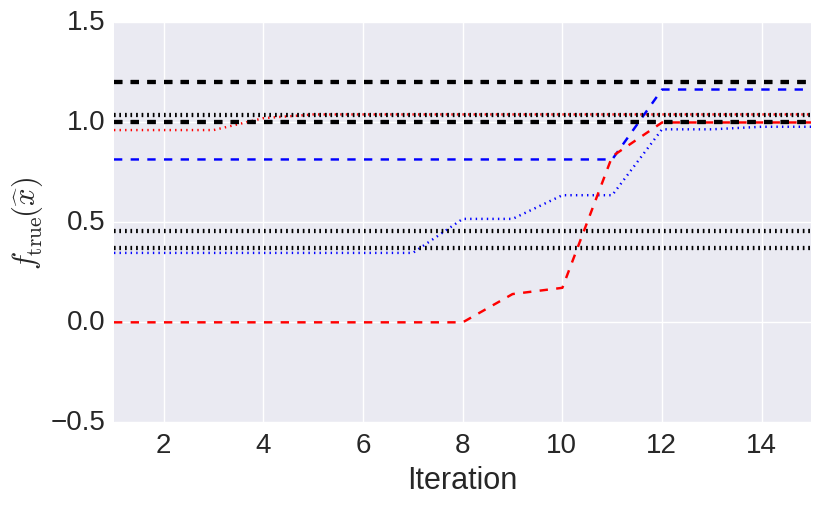
\includegraphics[width=0.6\textwidth]{figs/bayesopt/iteration_vs_error.png}&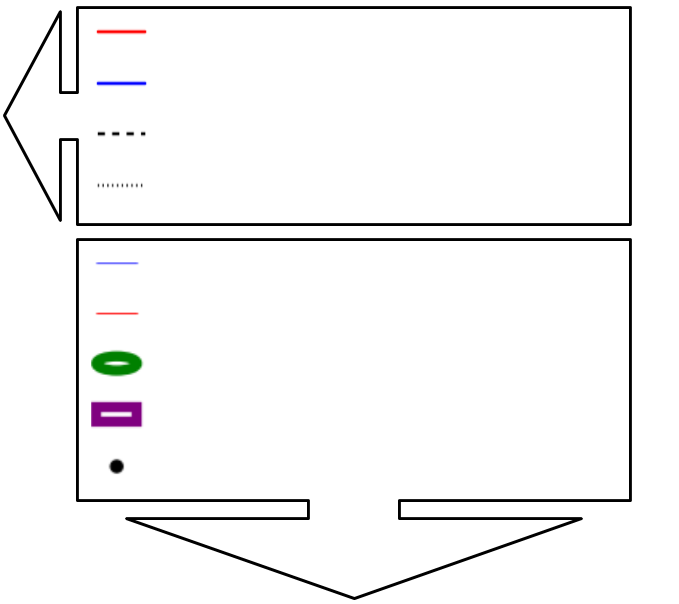
\includegraphics[width=0.4\textwidth]{figs/bayesopt/legend.png}
\put(-119,142){\scriptsize Drift Proposal}
\put(-119,130){\scriptsize Uniform Proposal}
\put(-119,117){\scriptsize Global Optimum}
\put(-119,105){\scriptsize Local Optima}
\put(-119,85){\scriptsize Ground Truth}
\put(-119,73){\scriptsize Posterior samples}
\put(-119,60){\scriptsize Next Probe}
\put(-119,48){\scriptsize Estimated Optimum}
\put(-119,36){\scriptsize Past Probes}
\end{tabular}
\begin{tabular}{llll}\hline 
\multicolumn{1}{|l|}{\raisebox{-0.5\height}{\includegraphics[width=0.3\textwidth]{figs/bayesopt/opt_sequence_uniform_trimodal_1.png}}}&
\multicolumn{1}{l|}{\raisebox{-0.5\height}{\includegraphics[width=0.3\textwidth]{figs/bayesopt/opt_sequence_uniform_trimodal_2.png}}}&
\multicolumn{1}{l|}{\raisebox{-0.5\height}{\includegraphics[width=0.3\textwidth]{figs/bayesopt/opt_sequence_uniform_trimodal_3.png}}} \\ \hline
\multicolumn{1}{|l|}{\raisebox{-0.5\height}{\includegraphics[width=0.3\textwidth]{figs/bayesopt/opt_sequence_uniform_trimodal_4.png}}}&
\multicolumn{1}{l|}{\raisebox{-0.5\height}{\includegraphics[width=0.3\textwidth]{figs/bayesopt/opt_sequence_uniform_trimodal_5.png}}}&
\multicolumn{1}{l|}{\raisebox{-0.5\height}{\includegraphics[width=0.3\textwidth]{figs/bayesopt/opt_sequence_uniform_trimodal_6.png}}} \\ \hline
\multicolumn{1}{|l|}{\raisebox{-0.5\height}{\includegraphics[width=0.3\textwidth]{figs/bayesopt/opt_sequence_uniform_trimodal_7.png}}}&
\multicolumn{1}{l|}{\raisebox{-0.5\height}{\includegraphics[width=0.3\textwidth]{figs/bayesopt/opt_sequence_uniform_trimodal_8.png}}}&
\multicolumn{1}{l|}{\raisebox{-0.5\height}{\includegraphics[width=0.3\textwidth]{figs/bayesopt/opt_sequence_uniform_trimodal_9.png}}} \\ \hline
\multicolumn{1}{|l|}{\raisebox{-0.5\height}{\includegraphics[width=0.3\textwidth]{figs/bayesopt/opt_sequence_uniform_trimodal_10.png}}}&
\multicolumn{1}{l|}{\raisebox{-0.5\height}{\includegraphics[width=0.3\textwidth]{figs/bayesopt/opt_sequence_uniform_trimodal_11.png}}}&
\multicolumn{1}{l|}{\raisebox{-0.5\height}{\includegraphics[width=0.3\textwidth]{figs/bayesopt/opt_sequence_uniform_trimodal_12.png}}} \\ \hline
\end{tabular}
\put(-387,130){\footnotesize$i = 2$}
\put(-255,130){\footnotesize$i = 3$}
\put(-123,130){\footnotesize$i = 4$}
\put(-387,62){\footnotesize$i = 5$}
\put(-255,62){\footnotesize$i = 6$}
\put(-123,62){\footnotesize$i = 7$}
\put(-387,-8){\footnotesize$i = 8$}
\put(-255,-8){\footnotesize$i = 9$}
\put(-123,-8){\footnotesize$i = 10$}
\put(-387,-78){\footnotesize$i = 11$}
\put(-255,-78){\footnotesize$i = 12$}
\put(-123,-78){\footnotesize$i = 13$}
\caption{Top: the estimated optimum over time. Blue and Red represent optimization with uniform and Gaussian drift proposals. Black lines indicate the local optima of the true functions. Bottom: a sequence of actions. Depicted are iterations 7-12 with uniform proposals.}\label{fig:bopt_results}
\end{figure}
In Fig. \ref{fig:bopt_results} we show results for our implementation of Bayesian Optimization 
with Thompson sampling. We compare two different proposal distributions, namely uniform proposals
and Gaussian drift proposals. We see that in this experiment, Gaussian drift is starting near 
the global optimum and drifts quickly towards it. (red curve, top panel of Fig. \ref{fig:bopt_results}).
Uniform proposals take longer to find the global optimum (blue curve, top panel of Fig. \ref{fig:bopt_results})
but we see that it can surpass the local optima of the curve\footnote{In fact, repeated experiments have
shown that when the Gaussian drift proposals starts near a local optimum, it gets stuck there. Uniform
proposals do not.}.
The bottom panel of Fig. \ref{fig:bopt_results} depicts a sequence of actions using uniform proposals.
The sequence illustrates the exploitation exploration trade-off that the implementation overcomes.
We start with complete uncertainty ($i=2$).
The Bayesian agent performs exploration until it gets a (wrong!) idea of where the optimum could be
(exploiting the local optima $i=5$ to $i=10$).
$i=11$ shows a change in tactic. The Bayesian agent, having exploited the local optima in previous
steps, is now reducing uncertainty in area it knows nothing about, eventually finding the global
optimum. 



%input{sections/BayesianOptimization.tex}
%\subsubsection{Thompson sampling framework}
%We now lay out the setup of Thompson sampling for Markov decision processes (MDPs).
An agent is to take a sequence of actions $a_1, a_2, \ldots$ from a (possibly infinite) set of possible actions $\Acal$.
After each action, a reward $r \in \R$ is received, according to an unknown conditional distribution $P_\true(r|a)$.
The agent's goal is to maximize the total reward received for all actions.
In Thompson sampling, the Bayesian agent accomplishes this by placing a prior distribution $P(\theta)$ on the possible ``contexts'' $\theta \in \Theta$.
Here a context is a believed model of the conditional distributions $\{P(r|a)\}_{a \in \Acal}$, or at least, a believed statistic of these conditional distributions which is sufficient for deciding an action $a$.
One example of such a sufficient statistic is the conditional mean $V(a|\theta) = \Ebkt{r|a,\theta}$, which can be thought of as a value function.
Thompson sampling thus has the following steps, repeated as long as desired:
\begin{enumerate}
  \item Sample a context $\theta \sim P(\theta)$.
  \item Choose an action $a \in \Acal$ which (approximately) maximizes $V(a|\theta) = \Ebkt{r|a,\theta}$.
  \item\label{itm:Thompson-conditioning}
    Let $r_\true$ be the reward received for action $a$.
    Update the believed distribution on $\theta$, i.e., $P(\theta) \gets P_\rmnew(\theta)$ where $P_\rmnew(\theta) = P\pn{\theta \mvert a \mapsto r_\true}$.
\end{enumerate}
Note that when $\Ebkt{r|a,\theta}$ (under the sampled value of $\theta$ for some points $a$) is far from the true value $\Ebkt[P_\true]{r|a}$, the chosen action $a$ may be far from optimal, but the information gained by probing action $a$ will improve the belief $\theta$.
This amounts to ``exploration.''
When $\Ebkt{r|a,\theta}$ is close to the true value except at points $a$ for which $\Ebkt{r|a,\theta}$ is low, exploration will be less likely to occur, but the chosen actions $a$ will tend to receive high rewards.
This amounts to ``exploitation.''
Roughly speaking, exploration will happen until the context $\theta$ is reasonably sure that the unexplored actions are probably not optimal, at which time the sampler will exploit by choosing actions in regions it knows to have high value.

Typically, when Thompson sampling is implemented, the search over contexts $\theta \in \Theta$ is limited by the choice of representation.
In traditional programming environments, $\theta$ often consists of a few numerical parameters for a family of distributions of a fixed functional form.
With work, a mixture of a few functional forms is possible; but without probabilistic programming machinery, implementing a rich context space $\Theta$ would be an unworkably large technical burden.
In a probabilstic programing language, however, the representation of heterogeneously structured or infinite-dimensional context spaces is quite natural.
Any computable model of the conditional distributions $\br{P(r|a)}_{a \in \Acal}$ can be represented as a stochastic procedure $(\lambda (a) \ldots)$.
Thus, for computational Thompson sampling, the most general context space $\widehat\Theta$ is the space of program texts.
Any other context space $\Theta$ has a natural embedding as a subset of $\widehat\Theta$.


%\subsubsection{Thompson sampling in Venture}
%
Because Venture supports sampling and inference on (stochastic-)procedure-valued random variables (and the generative models which produce those procedures), Venture can capture arbitrary context spaces as described above.
To demonstrate, we have implemented Thompson sampling in Venture in which the contexts $\theta$ are Gaussian processes over the action space $\Acal = \R$.
That is, $\theta = (\mu, K)$, where the mean $\mu$ is a computable function $\Acal \to \R$ and the covariance $K$ is a computable (symmetric, positive-semidefinite) function $\Acal \times \Acal \to \R$.
This represents a Gaussian process $\br{R_a}_{a \in \Acal}$, where $R_a$ represents the reward for action $a$.
% where for any finite subset $\br{a_i}_{i=1}^{n} \subset \Acal$, the marginal distribution on $\pn{R_{a_i}}$ is Gaussian with mean $\pn{\mu(a_i)}_{i=1}^{n}$ and covariance matrix $\begin{pmatrix} K(a_i,a_j) \end{pmatrix}_{1 \leq i,j \leq n}$.
Computationally, we represent a context not as a pair of infinite lookup tables for $\mu$ and $K$, but as a finite data structure $\theta = (K_\prior, \sigma, \ell, \abf_\past, \rbf_\past)$, where
\begin{itemize}
  \item $K_\prior = K_{\prior,\sigma,\ell}$ is a procedure, with parameters $\sigma,\ell$, to be used as the prior covariance function: $K_\prior(a,a') = \sigma^2 \exp\pn{-\frac{(a-a')^2}{2\ell^2}}$
  \item $\sigma$ and $\ell$ are (hyper)parameters for $K_\prior$
  \item $\abf_\past = \pn{a_i}_{i=1}^{n}$ are the previously probed actions
  \item $\rbf_\past = \pn{r_i}_{i=1}^{n}$ are the corresponding rewards
\end{itemize}
To simplify the treatment, we take prior mean $\mu_\prior \equiv 0$.  The mean and covariance for $\theta$ are then gotten by the usual conditioning formula:
\begin{align*}
  \mu(\abf)
  &= \mu\pn{\abf \mvert \abf_\past, \rbf_\past} \\
  &= K_\prior(\abf, \abf_\past)
     \,K_\prior(\abf_\past, \abf_\past)^{-1}
     \,\rbf_\past \\
  K(\abf, \abf)
  &= K\pn{\abf, \abf \mvert \abf_\past, \rbf_\past} \\
  &= K_\prior(\abf, \abf)
     - K_\prior(\abf, \abf_\past)
       \,K_\prior(\abf_\past, \abf_\past)^{-1}
       \,K_\prior(\abf_\past, \abf).
\end{align*}
Note that even in this simple example, the context space $\Theta$ is not a finite-dimensional parametric family, since the vectors $\abf_\past$ and $\rbf_\past$ grow as more samples are taken.
$\Theta$ is, however, quite easily representable as a computational procedure together with parameters and past samples, as we do in the representation $\theta = (K_\prior, \sigma, \ell, \abf_\past, \rbf_\past)$.


%\subsubsection{Implementation with \gpmem}
%
As a demonstration, we use Thompson sampling to optimize an unknown function $V(x)$ (the value function) using \gpmem.
(\textbf{TODO} we should not assume $V$ is deterministic, it would be easy enough to make it random or have it give noisy samples.)
We assume $V$ is made available to Venture as a black-box.
The code for optimizing $V$ is given in Listing \ref{alg:bayesopt}.
For step \ref{itm:Thompson-conditioning} of Thompson sampling, the Bayesian update, we not only condition on the new data (the chosen action $a$ and the received reward $r$), but also perform inference on the hyperparameters $\sigma, \ell$ using a Metropolis--Hastings sampler.
These two inference steps take 1 line of code: 0 lines to condition on the new data (as this is done automatically by \gpmem), and 1 line to call Venture's built-in \texttt{MH} operator.
The results are shown in Figure \ref{fig:bayesopt-sequence}.
We can see from the figure that, roughly speaking, each successive probe point $a$ is chosen either because the current model $V_\emu$ thinks it will have a high reward, or because the value of $V_\emu(a)$ has high uncertainty.
In the latter case, probing at $a$ decreases this uncertainty and, due to the smoothing kernel, also decreases the uncertainty at points near $a$.
We thus see that our Thompson sampler simultaneously learns the value function and optimizes it.

\begin{minipage}{\linewidth}
\small
\belowcaptionskip=-10pt
\begin{lstlisting}[frame=single,caption={
  Code for Bayesian optimization using \gpmem.
  %The procedure \texttt{V\_compute} probes \texttt{V} directly, thus improving the GP model \texttt{V\_emu}.
  %(\texttt{V\_emu\_pointwise} is simply a shortcut for sampling the GP model at a single point; \texttt{V\_emu} is more general, allowing joint samples to be taken at any set of points.)
  In the loop, \texttt{V\_compute} is called to probe the value of \texttt{V} at a new argument.
  The new argument, \texttt{(mc\_argmax V\_emu\_pointwise mc\_sampler)}, is a Monte Carlo estimate of the maximum pointwise sample of \texttt{V\_emu} (itself a stochastic quantity), with the Monte Carlo samples being drawn in this case uniformly between $-20$ and $20$.
  After each new call to \texttt{V\_compute}, the Metropolis--Hastings algorithm is used to perform inference on the hyperparameters of the covariance function in the GP model in light of the new conditioning data.
  Once enough calls to \texttt{V\_compute} have been made (in our case we stopped at 15 calls), we can inspect the full list of probed $(a,r)$ pairs with \texttt{extract\_stats}.
  The answer to our maximization problem is simply the pair having the highest $r$; but our algorithm also learns more potentially useful information.},mathescape,label=alg:bayesopt]
assume log_sf = tag('hyper, log(uniform_continuous(0, 10)))
assume log_l = tag('hyper, log(uniform_continuous(0, 10)))
assume se = make_squaredexp(log_sf, log_l)
assume blackbox_f = get_bayesopt_blackbox()
assume (f_compute, f_emu) = gpmem(blackbox_f, se)

define get_uniform_candidate = proc(prev_xs) {
  uniform_continuous(-20, 20)
}

define mc_argmax = proc(func, prev_xs) {
  // Monte Carlo estimator for the argmax of func.
  run(do(
    candidate_xs <- mapv(proc(i) {get_uniform_candidate(prev_xs)},
                         linspace(0, 19, 20)),
    candidate_ys <- mapv(func, candidate_xs),
    lookup(candidate_xs, argmax_of_array(candidate_ys))))
}

define emulator_point_sample = proc(x) {
  run(sample(lookup(
    f_emu(array(x)),
    0)))
}

infer repeat(15, do(pass,
     // Phase 2: Call f_compute on the next probe point
     predict f_compute(
                 mc_argmax(emulator_point_sample, '_)),
     // Phase 1: Hyperparameter inference
     mh('hyper, one, 50)))
\end{lstlisting}
\end{minipage}
      
\begin{figure}
\centering
    \includegraphics[height=0.8\textheight]{figs/BayesOpt_gpmem_sequence.png}
    \caption{
      Dynamics of Thompson sampling in Venture.
      The blue curve is the true function $V$, and the red region is a blending of 100 samples of the curve generated (jointly) by a GP-based emulator $V_\emu$.
      The left and right columns show the state of $V_\emu$ before and after hyperparameter inference is run on the new data, respectively.
      (We can see, for example, that after the seventh probe point, the Metropolis--Hastings sampler chose a ``crazy'' set of hyperparameters, which was corrected at the next inference step.)
      In the right column, the next chosen probe point is circled in green.
      Each successive probe point $a$ is the (stochastic) maximum of $V_\emu$, sampled pointwise and conditioned on the values of the previously probed points.
      Note that probes tend to happen at points either where the value of $V_\emu$ is high, or where $V_\emu$ has high uncertainty.
      }
    \label{fig:bayesopt-sequence}
\end{figure}



%We consider a true and  unknown reward function $r(x)$ that we estimate with a GP prior $\mathcal{GP}(0,K(\mathbf{x},\mathbf{x}))$. We denote past observations with $\mathcal{D} = \{(x;

\FloatBarrier

\section{Discussion}
This paper has shown that it is feasible and useful to embed Gaussian processes
in higher-order probabilistic programming languages by treating them as a kind
of statistical memoizer. It has described classic GP regression with both fully
Bayesian and MAP inference in a hierarchical hyperprior, as well as state-of-the-art
applications to discovering symbolic structure in time series and to Bayesian optimization.
All the applications share a common 50-line Python GP library and require fewer than 20 lines
of probabilistic code each.

These results suggest several research directions. First, it will be important
to develop versions of {\tt gpmem} that are optimized for larger-scale
applications. Possible approaches include the standard low-rank approximations
to the kernel matrix that are popular in machine learning~\citep{bui2014tree} as well
as more sophisticated sampling algorithms for approximate conditioning of the
GP~\citep{lawrence2009efficient}.
Second, it seems fruitful to abstract the notion of a ``generalizing" memoizer
from the specific choice of a Gaussian process model as the mechanism for
generalization. ``Generalizing" or statistical memoizers with custom regression techniques could be broadly useful in performance engineering and scheduling systems.
The timing data from performance benchmarks could be run through a generalizing memoizer by default.
This memoizer could be queried (and its output error bars examined) to inform the best strategy
for performing the computation or predict the likely runtime of long-running jobs.
 Third, the structure learning application suggests follow-on research in information
retrieval for structured data. It should be possible to build a time series search engine
that can handle search predicates such as ``has a rising trend starting around
1988" or ``is perodic during the 1990s".
The variation on the Automated Statistician presented in this paper can provide ranked result
sets for these sorts of queries because it tracks posterior uncertainty over structure and also
because the space of structural patterns that it can handle is easy to modify by making small
changes to a short VentureScript program.


The field of Bayesian nonparametrics offers a principled, fully Bayesian
response to the empirical modeling philosophy in machine learning~\citep{ghahramani2013bayesian},
where Bayesian inference is used to encode a state of broad ignorance rather
than a bias stemming from strong prior knowledge. It is perhaps surprising that
two key objects from Bayesian nonparametrics, Dirichlet processes and Gaussian
processes, fit naturally in probabilistic programming as variants of
memoization~\citep{roy2008stochastic}. It is not yet clear if the same will be true
for other processes, e.g. Wishart processes, or hierarchical Beta processes. We hope that the results in this paper encourage the development of other nonparametric libraries for higher-order probabilistic programming languages.

\myparagraph{Acknowledgements}
This research was supported by DARPA
  (under the XDATA and PPAML programs), IARPA (under research contract
  2015-15061000003), the Office of Naval Research (under research
  contract N000141310333), the Army Research Office (under agreement
  number W911NF-13-1-0212), the Bill \& Melinda Gates Foundation, and
  gifts from Analog Devices and Google.
\newpage
\section*{Appendix}
\subsection*{A Covariance Functions}
\begin{align}
&\kse &=& \sigma^2 \exp(-\frac{(x-x^\prime)^2}{2\ell^2}) \label{eq:SE}\\
&\klin &=&   \sigma^2(x x^\prime) \label{eq:LIN}\\
&k^{\text{constant}} &=&   \sigma^2\label{eq:C}\\
&\kwn &=& \sigma^2 \delta_{x,x^\prime} \label{eq:WN} \\
&k^{\text{rational quadratic}}  &=&    \sigma^2 \bigg(1 + \frac{(x - x^\prime)^2}{2 \alpha \ell^2} \bigg)^{-\alpha} 
&\label{eq:RQ} \\
&\kper &=&  \sigma^2 \exp \bigg( \frac{2 \sin^2 ( \pi (x - x^\prime)/p}{\ell^2} \bigg). \label{eq:PER}
\end{align}
From top to bottom: the squared-exponential covariance function (\ref{eq:SE}),
also know as smoothing kernel; the linear kernel (\ref{eq:LIN});  the constant 
kernel (\ref{eq:C}); the white noise
kernel (\ref{eq:WN}); the
rational quadratic kernel (\ref{eq:RQ}); and the periodic kernel (\ref{eq:PER}).


\subsection*{B Covariance Simplification}
\begin{minipage}{\linewidth}
\small
\belowcaptionskip=-10pt
\begin{lstlisting}[frame=single,mathescape,label=alg:simplify,basicstyle=\selectfont\ttfamily]
SE $\times$ SE                  $\rightarrow$ SE 
{SE,PER,C,WN} $\times$ WN       $\rightarrow$ WN
LIN $+$ LIN                $\rightarrow$ LIN
{SE,PER,C,WN,LIN} $\times$ C    $\rightarrow$  {SE,PER,C,WN,LIN} 
\end{lstlisting}
\end{minipage}
Rule 1 is derived as follows:
\begin{equation}
\begin{aligned}
\sigma_c^2 \exp(-\frac{(x-x^\prime)^2}{2\ell_c^2})  &=  \sigma_a^2 \exp(-\frac{(x-x^\prime)^2}{2\ell_a^2}) \times  \sigma_b^2 \exp(-\frac{(x-x^\prime)^2}{2\ell_b^2}) \\
&= \sigma_c^2 \exp(-\frac{(x-x^\prime)^2}{2\ell_a^2}) \times   \exp(-\frac{(x-x^\prime)^2}{2\ell_b^2}) \\
&= \sigma_c^2 \exp \bigg(-\frac{(x-x^\prime)^2}{2\ell_a^2} -\frac{(x-x^\prime)^2}{2\ell_b^2}\bigg) \\
&= \sigma_c^2 \exp \bigg(-\frac{(x-x^\prime)^2}{2\ell_c^2}\bigg) \\
\end{aligned}
\end{equation}
For stationary kernels that only depend on the lag vector between $x$ and $x^\prime$ it holds that multiplying such a kernel with a WN kernel we get another WN kernel (Rule 2). Take for example the SE kernel:
\begin{equation}
 \sigma_a^2 \exp \bigg(-\frac{(x-x^\prime)^2}{2\ell_c^2}\bigg) \times  \sigma_b \delta_{x,x^\prime} =  \sigma_a \sigma_b \delta_{x,x^\prime}
\end{equation}
Rule 3 is derived as follows:
\begin{equation}
 \theta_c (x \times x^\prime) = \theta_a (x \times x^\prime) + \theta_b (x \times x^\prime) 
\end{equation}
Multiplying any kernel with a constant obviously changes only the scale parameter of a kernel (Rule 4).


\subsection*{C The Struct-Operator}

\begin{align*}
\Struct(\klin) &= \text{LIN}\\
\Struct(\kper) &= \text{PER}\\
\Struct(\kse) &= \text{SE}\\
\Struct(\kwn) &= \text{WN}\\
\Struct(k^{\text{linear+periodic}}) &= \text{LIN}+\text{PER}\\
\Struct(k^{\text{linear} \times \text{periodic}}) &= \text{LIN}
\times\text{PER}
\end{align*}




\newpage
\subsection*{D Glossary}
\begin{tabular}{l l}
$\mathcal{N}$		&  (Multivariate-) Gaussian \\
$\mathcal{GP}$		&  Gaussian Process \\
$\mathbb{E}$		&  Expectation    \\
$x,x_i$ 			&  Scalar, possibly indexed with $i$   \\
$\xbf$				&  Column vector, training data:
regression input (also actions in section \ref{sec:thompson})    \\
$\ybf$				&  Column vector, training data:
regression output  (also rewards in section \ref{sec:thompson})    \\
$\Acal$				& A set of possible actions \\

 $\xprime$			&  Column vector, unseen test input: regression input    \\
 $\yprime$			&  Column vector, sample from predictive posterior, that
is a sample from\\
&$\mathcal{N}(\mupost,\Kpost)$    \\

$\xstar$         &  Column vector, unseen test
input: regression input before any data\\
&has been observed    \\
$\ystar$		&  Column vector, sample from the predictive prior
conditioned on $\thetabf$\\
& and unseen test input $\xstar$ \\
$\Dbf$		&  Data matrix $[\xbf\; \ybf]$ \\

$\mu(x)$                 &  Mean function \\
$\thetabf_{\text{mean}}$	&  hyper-parameters for a mean function
\\
$k \text{ or } k(x_i,x_j)$	&  a covariance function or kernel, that is a
function that takes two scalars as input \\

$\thetabf$			&  hyper-parameters for a
kernel/covariacne function (also semicontext in section \ref{sec:thompson})\\
$k(x_i,x_j \midtheta )$		&  a kernel conditioned on its
hyper-parameters \\
$K(\xbf,\xprime \midtheta )$    &  Function outputting a matrix of dimension $I \times J$
with entries $k(x_i,x_j \midtheta )$;\\
&with $x_i \in \xbf$ and $x_j \in \xprime$ where $I$ and $J$ indicate the length
of the\\
&column vectors $\xbf$ and
$\xprime$ \\

$\ktheta$			&  a covariance function parameterized with
$\thetabf$\\

$\Ktheta\text{ or }\Kbf_{(\thetabf,\xbf,\xbf)}$		&  covariance matrix
computed with by $K(\xbf,\xbf \midtheta)$   \\
$\mupost$ &  Posterior mean vector for $\yprime \mid \xbf, \xprime, \ybf, \thetabf$ \\
$\Kpost$     &  Posterior covariance matrix for $\yprime \mid \xbf, \xprime, \ybf, \thetabf$ \\
$\Lbf$			&lower triangular matrix, given by the Cholesky factorization as 
$\Lbf\coloneqq \text{chol}(\Ktheta)$\\

$\kse$ &  Squared exponential covariance function  \\
$\klin$ &  Linear covariance function  \\
$k^{\text{constant}}$ &  Constant covariance function  \\
$\kwn$ &  White noise covariance function  \\
$k^{\text{rational quadratic}}$  &  Rational quadratic covariance function  \\
$\kper$ &  Periodic covariance function  \\

SE			&  Symbolic expression for the squared exponential covariance function  \\
LIN		        &  Symbolic expression for the linear covariance function  \\
PER		        &  Symbolic expression for the periodic covariance function  \\
RQ		        &  Symbolic expression for the rational quadratic covariance function  \\
C		        &  Symbolic expression for the constant covariance function  \\
WN		        &  Symbolic expression for the white noise covariance function  \\
\end{tabular}
\newpage
\begin{tabular}{l l}
$\land$                &  Logical and \\
$\lor$                 &  Logical or \\
$\Krv$			& Random variable over kernel functions \\
kernel functions \\
Parse$(k)$		& Parse the structure for kernel $k$ \\
Simplify$(k)$		& Simplify the functional expression for kernel $k$ \\
Struct$(k)$		& Symbolic interpretation for kernel $k$ \\
$\Cont(k,k^t)$          & A kernel $k^t$ contains the global kernel structure
$k$\\
$\SEK$			&  Operator to check if $\Struct(\Ksrv=k)=\text{SE}$\\
$\LINK$			&  Operator to check if $\Struct(\Ksrv=k)=\text{LIN}$\\
$\PERK$			&  Operator to check if $\Struct(\Ksrv=k)=\text{PER}$\\
$\WNK$			&  Operator to check if $\Struct(\Ksrv=k)=\text{WN}$\\
BK			& A set of base kernels \\
$\Sbf$			& A subset of BK, randomly selected \\
$\Omegabf$		& Random variable for composition operators, in our
case that is kernel addition\\
&and multiplication $\{+,\times\}$\\
$\Gamma(\alpha,\beta)$ & Gamma distribution with shape parameter $\alpha$ and
rate $\beta$ \\

$\ell$			& Length-scale parameter for $\kse$  \\
$sf$			& Scale factor parameter\\
$\ttheta \in \Theta$    & Context in Thompson sampling\\ 
$\Theta$    & Context space\\ 
$V$			& Value function\\
$Q_\proposal$		& Proposal distribution\\
$E$			& Energy function\\
$s$			& Temperature parameter \\
\end{tabular}

%\subsection*{C Additional Structure Learning Results}
%\begin{figure}
\includegraphics[width=\textwidth]{figs/posterior_samples_airline.png}
\caption{Data (black x) and posterior samples (red) for the airline data set.}
\end{figure}


\begin{figure}
        \centering
        \begin{subfigure}{0.49\textwidth} \centering
                \includegraphics[width=0.9\textwidth]{figs/airline_struct_1.pdf}
        \end{subfigure}
	\begin{subfigure}{0.49\textwidth} \centering
                \includegraphics[width=0.8\textwidth]{figs/airline_struct_2.pdf}
        \end{subfigure}
        \caption{We see two possible hypotheses for the composite structure of $\mathbf{K}$. (a) Most frequent sample drawn from the posterior on structure. We have found two global components. First, a smooth trend (LIN $\times$ SE) with a non-linear increasing slope. Second, a periodic component with increasing variation and noise. (b) Second most frequent sample drawn from the posterior on structure. We found one global component. It is comprised of local changes that are periodic and with changing variation.}\label{fig:posterior_twosamples}
\end{figure}

\newpage
\bibliography{VentureGP.01}
\bibliographystyle{apalike}
\end{document}
